% Options for packages loaded elsewhere
\PassOptionsToPackage{unicode}{hyperref}
\PassOptionsToPackage{hyphens}{url}
\PassOptionsToPackage{dvipsnames,svgnames*,x11names*}{xcolor}
%
\documentclass[
  10pt,
]{article}
\usepackage{lmodern}
\usepackage{amssymb,amsmath}
\usepackage{ifxetex,ifluatex}
\ifnum 0\ifxetex 1\fi\ifluatex 1\fi=0 % if pdftex
  \usepackage[T1]{fontenc}
  \usepackage[utf8]{inputenc}
  \usepackage{textcomp} % provide euro and other symbols
\else % if luatex or xetex
  \usepackage{unicode-math}
  \defaultfontfeatures{Scale=MatchLowercase}
  \defaultfontfeatures[\rmfamily]{Ligatures=TeX,Scale=1}
\fi
% Use upquote if available, for straight quotes in verbatim environments
\IfFileExists{upquote.sty}{\usepackage{upquote}}{}
\IfFileExists{microtype.sty}{% use microtype if available
  \usepackage[]{microtype}
  \UseMicrotypeSet[protrusion]{basicmath} % disable protrusion for tt fonts
}{}
\makeatletter
\@ifundefined{KOMAClassName}{% if non-KOMA class
  \IfFileExists{parskip.sty}{%
    \usepackage{parskip}
  }{% else
    \setlength{\parindent}{0pt}
    \setlength{\parskip}{6pt plus 2pt minus 1pt}}
}{% if KOMA class
  \KOMAoptions{parskip=half}}
\makeatother
\usepackage{xcolor}
\IfFileExists{xurl.sty}{\usepackage{xurl}}{} % add URL line breaks if available
\IfFileExists{bookmark.sty}{\usepackage{bookmark}}{\usepackage{hyperref}}
\hypersetup{
  colorlinks=true,
  linkcolor=red,
  filecolor=Maroon,
  citecolor=Blue,
  urlcolor=blue,
  pdfcreator={LaTeX via pandoc}}
\urlstyle{same} % disable monospaced font for URLs
\usepackage[margin=1in]{geometry}
\usepackage{longtable,booktabs}
% Correct order of tables after \paragraph or \subparagraph
\usepackage{etoolbox}
\makeatletter
\patchcmd\longtable{\par}{\if@noskipsec\mbox{}\fi\par}{}{}
\makeatother
% Allow footnotes in longtable head/foot
\IfFileExists{footnotehyper.sty}{\usepackage{footnotehyper}}{\usepackage{footnote}}
\makesavenoteenv{longtable}
\usepackage{graphicx,grffile}
\makeatletter
\def\maxwidth{\ifdim\Gin@nat@width>\linewidth\linewidth\else\Gin@nat@width\fi}
\def\maxheight{\ifdim\Gin@nat@height>\textheight\textheight\else\Gin@nat@height\fi}
\makeatother
% Scale images if necessary, so that they will not overflow the page
% margins by default, and it is still possible to overwrite the defaults
% using explicit options in \includegraphics[width, height, ...]{}
\setkeys{Gin}{width=\maxwidth,height=\maxheight,keepaspectratio}
% Set default figure placement to htbp
\makeatletter
\def\fps@figure{htbp}
\makeatother
\setlength{\emergencystretch}{3em} % prevent overfull lines
\providecommand{\tightlist}{%
  \setlength{\itemsep}{0pt}\setlength{\parskip}{0pt}}
\setcounter{secnumdepth}{5}
\usepackage{placeins}
\usepackage{fancyhdr}
\usepackage{setspace}
\onehalfspacing
\usepackage{chngcntr}
\usepackage{subfig}
\usepackage{float}
\usepackage{lscape}
\newcommand{\blandscape}{\begin{landscape}}
\newcommand{\elandscape}{\end{landscape}}
\newcommand{\onlythepage}{\arabic{page}}
\newcommand*{\secref}[1]{Section~\ref{#1}}
\raggedbottom
\usepackage{amsmath}
\usepackage{amssymb}
\usepackage[utf8]{inputenc}
\usepackage[greek,english]{babel}
\usepackage{enumerate}
\newcommand{\qed}{\hfill $\blacksquare$}
\renewcommand{\thepage}{(\thesection):\arabic{page}}
\usepackage{graphicx}
\usepackage{pdfpages}
\usepackage{cancel}
\usepackage{xcolor}
\usepackage{soul}
\usepackage[normalem]{ulem}
\usepackage{mathtools}
\usepackage{booktabs}
\usepackage{longtable}
\usepackage{array}
\usepackage{multirow}
\usepackage{wrapfig}
\usepackage{float}
\usepackage{colortbl}
\usepackage{pdflscape}
\usepackage{tabu}
\usepackage{threeparttable}
\usepackage{threeparttablex}
\usepackage[normalem]{ulem}
\usepackage{makecell}
\usepackage{xcolor}

\author{}
\date{\vspace{-2.5em}}

\begin{document}

\pagenumbering{gobble}

\begin{centering}

\vspace{2 cm}

\Large

{\bf Økonometri II}

\vspace{1 cm}
{\it Eksamensopgaver}

\Large


\vspace{2 cm}

\normalsize


\vspace{12 cm}

\normalsize
Aalborg University Business School \\
Kasper Kann og Daniel Behr \\
Student ID: 20134818 og 20195227 \\
januar 2022

\vspace{2 cm}



\vspace{2 cm}


\end{centering}

\newpage

\pagestyle{fancy}

\fancyhead[LE,RO]{}
\fancyhead[LO,RE]{}

\renewcommand{\headrulewidth}{0.4pt}
\renewcommand{\footrulewidth}{0pt}

\pagenumbering{roman}

\FloatBarrier
\newpage

\FloatBarrier
\newpage

\fancyhead[CO,CE]{Indholdsfortegnelse}

\setcounter{tocdepth}{4}

\tableofcontents

\newpage
\FloatBarrier

\pagenumbering{arabic}

\FloatBarrier

\fancyhead[CO,CE]{Økonometri II eksamensopgaver}
\rfoot{\textit{\copyright\ Kann og Behr \ 2021}}

\hypertarget{eksamensopgave-1}{%
\section{Eksamensopgave 1}\label{eksamensopgave-1}}

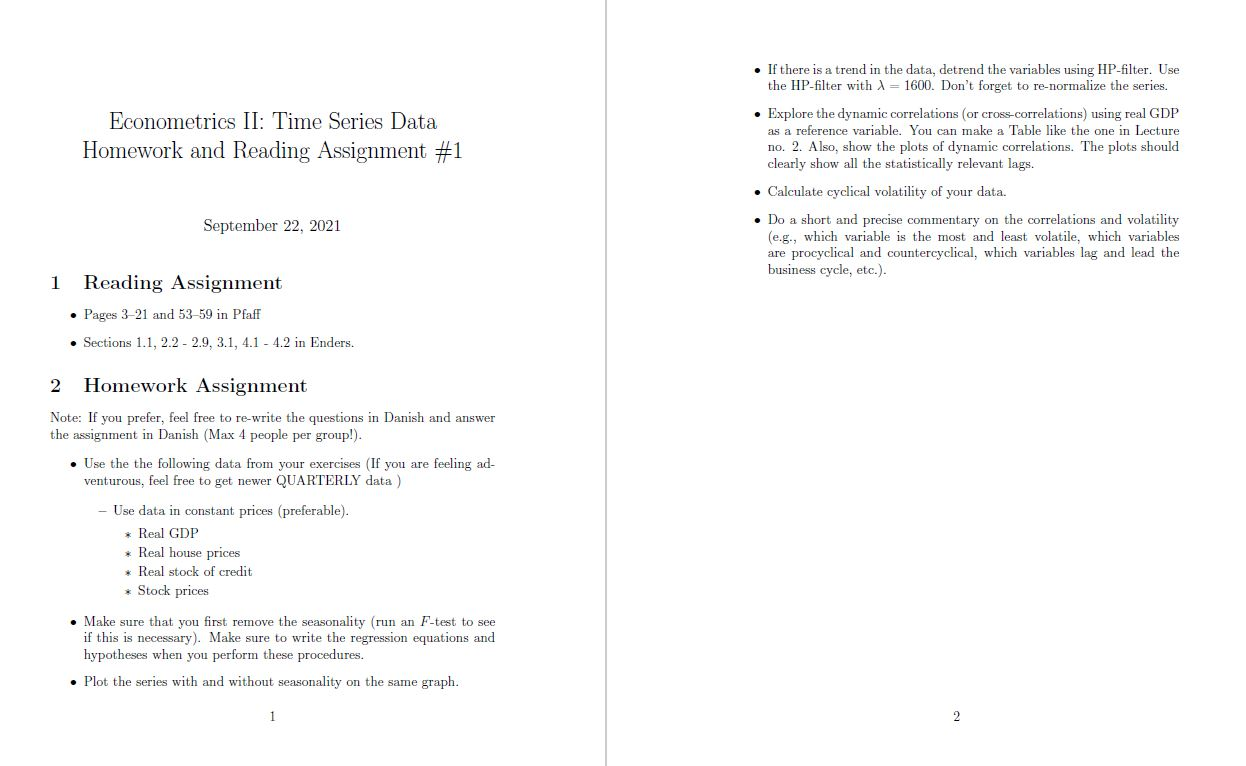
\includegraphics{Eksamen1.jpg} \newpage

\hypertarget{use-the-following-data-from-your-exercises}{%
\subsection{Use the following data from your
exercises:}\label{use-the-following-data-from-your-exercises}}

Her har vi valgt dataet fra vores øvelser. Det indeholder:\\
- Real GDP\\
- Real House prices\\
- Real stock og credit\\
- Stock prices\\

\hypertarget{make-sure-that-you-first-remove-the-seasonality-run-an-f-test-to-see-if-this-is-necessary.-make-sure-to-write-the-regression-equations-and-hypotheses-when-you-perform-these-procedures.}{%
\subsection{Make sure that you first remove the seasonality (run an
F-test to see if this is necessary). Make sure to write the regression
equations and hypotheses when you perform these
procedures.}\label{make-sure-that-you-first-remove-the-seasonality-run-an-f-test-to-see-if-this-is-necessary.-make-sure-to-write-the-regression-equations-and-hypotheses-when-you-perform-these-procedures.}}

\leavevmode

Først prøver vi at undersøge om der er seasonality i vores data ved
hjælp af dummy-variabel metoden. Metoden kan opstilles:
\[BNP_t = \alpha+\beta_2D_2+\beta_3D_3+\beta_4D_4+\epsilon_t\]
\[Huspriser_t = \alpha+\beta_2D_2+\beta_3D_3+\beta_4D_4+\epsilon_t\]
\[kredit_t = \alpha+\beta_2D_2+\beta_3D_3+\beta_4D_4+\epsilon_t\]
\[aktiepriser_t = \alpha+\beta_2D_2+\beta_3D_3+\beta_4D_4+\epsilon_t\]
\textbf{Nulhypotese} \[
H_0 : \beta_2 = \beta_3 = \beta_4 = 0 
\tag{No seasonality} \] \textbf{Alternativ hypotese} \[
H_1 : \beta_2 \neq \beta_3 \neq \beta_4 \neq 0 
\tag{Seasonality} \]

F-testen går ind og bruger dummy variablerne ved at sætte et enkelt
kvartal til at være 1, fx. \(D_2=1\), og sætter de resterende til at
være 0. Det betyder at der kun fåes data fra et bestemt kvartal i
regressionen, og man kigger derfor på kvartalerne individuelt istedet
for at kigge på den samlede tidsserie. Man kan derfor finde ud af om
kvartalerne i sig selv er signifikante eller ej. Hvis de er
signifikante, så vil der være seasonality i det pågældende kvartal.

Ved at plotte vores tidsserie kan vi se om der kan være en tedens til
seasonality eller ej.\\

\begin{figure}[H]

{\centering \includegraphics[width=0.9\linewidth]{figures/unnamed-chunk-2-1} 

}

\caption{\label{fig:fig1}Plot af vores data}\label{fig:unnamed-chunk-2}
\end{figure}

I figur \ref{fig:fig1} kan vi se alt vores data og inspicere det for
seasonality. Umiddelbart kan det ikke ses, at der skulle være
seasonality i andet end BNP. Dette vil vi dog teste yderligere med en
F-test.

Kører F-test for alle variable:

\begin{table}[!htbp] \centering 
  \caption{Linæer regression med BNP} 
  \label{tab:tabel1} 
\begin{tabular}{@{\extracolsep{5pt}}lc} 
\\[-1.8ex]\hline 
\hline \\[-1.8ex] 
 & \multicolumn{1}{c}{\textit{Dependent variable:}} \\ 
\cline{2-2} 
\\[-1.8ex] & BNP\_ts \\ 
\hline \\[-1.8ex] 
 BNP\_q1 & $-$8,861.92 (17,443.13) \\ 
  BNP\_q2 & $-$3,495.05 (17,506.68) \\ 
  BNP\_q3 & $-$9,262.14 (17,506.68) \\ 
  Constant & 245,469.00$^{***}$ (12,379.09) \\ 
 \hline \\[-1.8ex] 
R$^{2}$ & 0.001 \\ 
Adjusted R$^{2}$ & $-$0.01 \\ 
Residual Std. Error & 102,080.60 (df = 269) \\ 
F Statistic & 0.13 (df = 3; 269) \\ 
\hline 
\hline \\[-1.8ex] 
\textit{Note:}  & \multicolumn{1}{r}{$^{*}$p$<$0.1; $^{**}$p$<$0.05; $^{***}$p$<$0.01} \\ 
\end{tabular} 
\end{table}

Tabel \ref{tab:tabel1} viser, at BNP ikke har nogle signifikante
værdier, så er der ikke seasonality i vores data. Dette giver også
mening, fordi vi i ikke har en økonomi, som er stærk præget af sæsoner.
Et eksempel på dette kunne være et land, som afhænger meget af landbrug
eller turisme. I tabellen er det estimatoren der står udenfor
(−8,861.92), og standard fejlen der står i parantes (17,443.13), mens
p-værdier er markeret med stjerner. \newpage

\begin{table}[!htbp] \centering 
  \caption{Linæer regression med kredit} 
  \label{tab:tabel2} 
\begin{tabular}{@{\extracolsep{5pt}}lc} 
\\[-1.8ex]\hline 
\hline \\[-1.8ex] 
 & \multicolumn{1}{c}{\textit{Dependent variable:}} \\ 
\cline{2-2} 
\\[-1.8ex] & kredit\_ts \\ 
\hline \\[-1.8ex] 
 kredit\_q1 & $-$2,491.25 (150,063.10) \\ 
  kredit\_q2 & $-$18,603.02 (150,609.80) \\ 
  kredit\_q3 & $-$12,516.77 (150,609.80) \\ 
  Constant & 1,243,937.00$^{***}$ (106,497.20) \\ 
 \hline \\[-1.8ex] 
R$^{2}$ & 0.0001 \\ 
Adjusted R$^{2}$ & $-$0.01 \\ 
Residual Std. Error & 878,198.60 (df = 269) \\ 
F Statistic & 0.01 (df = 3; 269) \\ 
\hline 
\hline \\[-1.8ex] 
\textit{Note:}  & \multicolumn{1}{r}{$^{*}$p$<$0.1; $^{**}$p$<$0.05; $^{***}$p$<$0.01} \\ 
\end{tabular} 
\end{table}

Tabel \ref{tab:tabel2} viser, at kredit har ikke nogle signifikante
værdier, og der derfor heller ikke er seasonality i kredit. Hvis der
skulle have været seasonality i kredit, så skulle der også have været
seasonality i nogle af de variable, som kredit er korrelerede med. Det
kunne fx. være BNP eller huspriser.

\begin{table}[!htbp] \centering 
  \caption{Linæer regression med huspriser} 
  \label{tab:tabel3} 
\begin{tabular}{@{\extracolsep{5pt}}lc} 
\\[-1.8ex]\hline 
\hline \\[-1.8ex] 
 & \multicolumn{1}{c}{\textit{Dependent variable:}} \\ 
\cline{2-2} 
\\[-1.8ex] & huspriser\_ts \\ 
\hline \\[-1.8ex] 
 huspriser\_q1 & $-$0.38 (3.06) \\ 
  huspriser\_q2 & $-$0.68 (3.07) \\ 
  huspriser\_q3 & $-$0.35 (3.07) \\ 
  Constant & 48.46$^{***}$ (2.17) \\ 
 \hline \\[-1.8ex] 
R$^{2}$ & 0.0002 \\ 
Adjusted R$^{2}$ & $-$0.01 \\ 
Residual Std. Error & 17.90 (df = 269) \\ 
F Statistic & 0.02 (df = 3; 269) \\ 
\hline 
\hline \\[-1.8ex] 
\textit{Note:}  & \multicolumn{1}{r}{$^{*}$p$<$0.1; $^{**}$p$<$0.05; $^{***}$p$<$0.01} \\ 
\end{tabular} 
\end{table}

Tabel \ref{tab:tabel3} viser, at huspriser har ikke nogle siknifikante
værdier, og derfor heller ikke har seasonality i sig. Man kunne
argumentere for, at det muligvis er nemmere at sælge boliger om sommeren
og der derfor kunne være tendens til seasonality, men dette kan dog ikke
bevises empirisk, og det må derfor være så små stigninger, at de ikke er
signifikante. \newpage

\begin{table}[!htbp] \centering 
  \caption{Linæer regression med aktiepriser} 
  \label{tab:tabel4} 
\begin{tabular}{@{\extracolsep{5pt}}lc} 
\\[-1.8ex]\hline 
\hline \\[-1.8ex] 
 & \multicolumn{1}{c}{\textit{Dependent variable:}} \\ 
\cline{2-2} 
\\[-1.8ex] & aktiepriser\_ts \\ 
\hline \\[-1.8ex] 
 aktiepriser\_q1 & 4.26 (34.17) \\ 
  aktiepriser\_q2 & $-$2.81 (34.30) \\ 
  aktiepriser\_q3 & $-$2.84 (34.30) \\ 
  Constant & 139.30$^{***}$ (24.25) \\ 
 \hline \\[-1.8ex] 
R$^{2}$ & 0.0002 \\ 
Adjusted R$^{2}$ & $-$0.01 \\ 
Residual Std. Error & 199.97 (df = 269) \\ 
F Statistic & 0.02 (df = 3; 269) \\ 
\hline 
\hline \\[-1.8ex] 
\textit{Note:}  & \multicolumn{1}{r}{$^{*}$p$<$0.1; $^{**}$p$<$0.05; $^{***}$p$<$0.01} \\ 
\end{tabular} 
\end{table}

Til sidst kan vi i Tabel \ref{tab:tabel4} se på aktiepriserne, at vi
ikke har noget seasonality. Når man kigger på de generelle aktiepriser
giver dette god mening. Hvis man skulle finde seasonality i aktier, så
ville man skulle kigge på specifikke aktier hvis indkomst afhænger af
sæsonindtjening.\\
~\\
Hvis vi havde haft seasonaility kan vi bruge residualerne til at fjerne
dette, og man ville kunne lave en sammenligning bagefter.

\newpage

\hypertarget{plot-the-series-with-and-without-seasonality-on-the-same-graph.}{%
\subsection{Plot the series with and without seasonality on the same
graph.}\label{plot-the-series-with-and-without-seasonality-on-the-same-graph.}}

Da vi ikke har seasonality i vores data, er dette lidt en hypotetisk
opgave, men vi vil stadigvæk udføre den for alle vores variable.

\begin{figure}[H]

{\centering \includegraphics[width=0.9\linewidth]{figures/unnamed-chunk-9-1} 

}

\caption{\label{fig:fig2}Plot af vores data uden/med sæsonjusteret variable}\label{fig:unnamed-chunk-9}
\end{figure}

I figur \ref{fig:fig2} kan vi se, at den sæsonjusterede og den
oprindelige data følger hinanden i alle tilfælde. Konklusionen må derfor
være, at der ikke er seasonality i nogle af vores variable. \newpage

\hypertarget{if-there-is-a-trend-in-the-data-detrend-the-variables-using-hp-filter.-use-the-hp-filter-with-lambda-1600.-dont-forget-to-re-normalize-the-series}{%
\subsection{\texorpdfstring{If there is a trend in the data, detrend the
variables using HP-filter. Use the HP-filter with \(\lambda = 1600\).
Don't forget to re-normalize the
series}{If there is a trend in the data, detrend the variables using HP-filter. Use the HP-filter with \textbackslash lambda = 1600. Don't forget to re-normalize the series}}\label{if-there-is-a-trend-in-the-data-detrend-the-variables-using-hp-filter.-use-the-hp-filter-with-lambda-1600.-dont-forget-to-re-normalize-the-series}}

Bare ved at se på vores plots fra tidligere opgaver, kan vi se, at de
fleste variabler har en opadgående trend efter et vist tidspunkt. Vi vil
derfor detrende med \hyperref[sec:hpfilter]{HP-filteret.}

\begin{figure}[H]

{\centering \includegraphics[width=0.9\linewidth]{figures/unnamed-chunk-11-1} 

}

\caption{\label{fig:fig3}Normal data, data med hp-trend og detrended data}\label{fig:unnamed-chunk-11}
\end{figure}

På figur \ref{fig:fig3} kan vi se, hvordan afvigelserne(de sorte
prikker) svinger fra trenden(den røde) i den blå linje. Dette kan bedre
vises, hvis vi laver 4 nye figurer, hvor vi laver trenden til en
nullinje og undlader selve trend-linjen. Dette kan ses nedenfor:

\begin{figure}[H]

{\centering \includegraphics[width=0.9\linewidth]{figures/unnamed-chunk-12-1} 

}

\caption{\label{fig:fig4}Cykliske afvigelser fra trenden(nullinjen)}\label{fig:unnamed-chunk-12}
\end{figure}

På figur \ref{fig:fig4} har vi kun de cykliske udsving fra trenden. Her
ser det ud til, at BNP har flere udsving end huspriser, kredit og
aktiepriser, og derfor kan være mere volatil. Dog skal vi huske på, at
BNP er en del af konjunkturcyklerne, mens huspriser, kredit og
aktiepriser er en del af de finansielle cykler, som er 3-4 gange så
lange som en konjunkturcyklen (Borio, 2012).

\newpage

\hypertarget{explore-the-dynamic-correlations-or-cross-correlations-using-real-gdp-as-a-reference-variable.-you-can-make-a-table-like-the-one-in-lecture-no.-2.-also-show-the-plots-of-dynamic-correlations.-the-plots-should-clearly-show-all-the-statistically-relevant-lags.}{%
\subsection{Explore the dynamic correlations (or cross-correlations)
using real GDP as a reference variable. You can make a Table like the
one in Lecture no. 2. Also, show the plots of dynamic correlations. The
plots should clearly show all the statistically relevant
lags.}\label{explore-the-dynamic-correlations-or-cross-correlations-using-real-gdp-as-a-reference-variable.-you-can-make-a-table-like-the-one-in-lecture-no.-2.-also-show-the-plots-of-dynamic-correlations.-the-plots-should-clearly-show-all-the-statistically-relevant-lags.}}

Med krydskorrelationer kan vi se, hvilke variabler, der er afhængige af
hinanden, og hvordan de opfører sig i forhold til hinanden. I denne
opgave skal vi se, hvordan de er afhængige af BNP.

\begin{figure}[H]

{\centering \includegraphics[width=0.9\linewidth]{figures/unnamed-chunk-13-1} 

}

\caption{\label{fig:fig5}Krydskorrelation med BNP som referencevariabel}\label{fig:unnamed-chunk-13}
\end{figure}

På figur \ref{fig:fig5} kan vi se, at BNP leder kredit ved lag -4, mens
huspriser leder BNP ved lag 1 og aktiepriserne leder BNP ved lag 2.\\
Kredit reagerer altså et år(4 kvartaler) langsommere end BNP på stød til
økonomien, mens BNP reagerer hhv. 1 og 2 kvartaler langsommere end
huspriser og BNP.

\newpage

De specifikke korrelationer kan ses på tabel 5 nedenfor:

\begin{longtable}[]{@{}rlll@{}}
\caption{Krydskorrelation med BNP som referencevariabel}\tabularnewline
\toprule
lags & kredit & huspriser & aktiepriser\tabularnewline
\midrule
\endfirsthead
\toprule
lags & kredit & huspriser & aktiepriser\tabularnewline
\midrule
\endhead
-6 & \textcolor{black}{0.322624405026198} &
\textcolor{black}{0.0804670507129494} &
\textcolor{black}{-0.0700658363574013}\tabularnewline
-5 & \textcolor{red}{0.340445443068852} &
\textcolor{black}{0.105807471254522} &
\textcolor{black}{-0.0552092784555296}\tabularnewline
-4 & \textcolor{red}{0.347576928435119} &
\textcolor{black}{0.200597558585477} &
\textcolor{black}{-0.0279506342709945}\tabularnewline
-3 & \textcolor{black}{0.315365974117988} &
\textcolor{black}{0.324016730440721} &
\textcolor{black}{0.0475511435082158}\tabularnewline
-2 & \textcolor{black}{0.30855573762351} &
\textcolor{black}{0.345145646223187} &
\textcolor{black}{0.145257103812127}\tabularnewline
-1 & \textcolor{black}{0.275870708070284} &
\textcolor{black}{0.378525660775729} &
\textcolor{black}{0.198240312334703}\tabularnewline
0 & \textcolor{black}{0.219161104570844} &
\textcolor{red}{0.444958892866889} &
\textcolor{black}{0.262078851534217}\tabularnewline
1 & \textcolor{black}{0.112006483372774} &
\textcolor{red}{0.484855699495344} &
\textcolor{red}{0.327392278535095}\tabularnewline
2 & \textcolor{black}{0.0428805631214971} &
\textcolor{black}{0.383645980149364} &
\textcolor{red}{0.337795781593063}\tabularnewline
3 & \textcolor{black}{-0.0285672810062044} &
\textcolor{black}{0.257949300288704} &
\textcolor{black}{0.279232463256133}\tabularnewline
4 & \textcolor{black}{-0.0955701225755898} &
\textcolor{black}{0.169916828419852} &
\textcolor{black}{0.202644366328116}\tabularnewline
5 & \textcolor{black}{-0.160182622021407} &
\textcolor{black}{0.118309996479215} &
\textcolor{black}{0.137015383913197}\tabularnewline
6 & \textcolor{black}{-0.178363765944123} &
\textcolor{black}{-0.00683764282901576} &
\textcolor{black}{0.0518009882396847}\tabularnewline
\bottomrule
\end{longtable}

Her kan vi se, som vi allerede har bekræftet, at det er ved de
rød-markerede lags, der er størst korrelation mellem de forskellige
variabel. Vi kan altså se at Kredit har størst korrelation ved -4 og -5
lags. Huspriser har størst korrelation ved 0 og 1 lag. Aktiepriser har
størst korrelation med BNP ved 1 og 2 lags. Der tegner sig altså et
mønster af, at Huspriser og aktiepriser korrelerer nogenlunde på samme
tid mens Kredit reagerer 4 til 5 kvartaler langsommere end BNP. BNP
``leder'' altså kredit.

For at udpensle dette kan vi også prøve at plotte de cykliske bevægelser
i figur \ref{fig:fig6} på næste side, så vi kan se, hvordan udsvingene
fungerer og hvordan variablerne reagerer overfor hinanden:

\begin{figure}[H]

{\centering \includegraphics[width=0.9\linewidth]{figures/unnamed-chunk-16-1} 

}

\caption{\label{fig:fig6}Cykliske afvigelser fra trenden}\label{fig:unnamed-chunk-16}
\end{figure}

I figur \ref{fig:fig6} har vi i den øverste figur lavet et glidende
gennemsnit af BNP for at mindske de mange cykliske udsving. Her er det
svært at sammenligne variablene, fordi tidsperioden er lang. I den
nederste figur tilføjer vi et glidende gennemsnit til aktiepriser for at
gøre det endnu nemmere at sammenligne, hvordan de forskellige variable
reagerer over for stød. Vi er ikke direkte interesseret i udsvingenes
størrelse, så glidende gennemsnit vil ikke påvirke tidligere analyse fra
krydskorrelationen i figur \ref{fig:fig5}.\\
På figur \ref{fig:fig6} kan vi bekæfte, hvad vi allerede har set i
tidligere krydskorrelationer. Aktiepriser og huspriser leder BNP, mens
BNP leder kredit. Aktiepriser og huspriser reagerer altså på et stød 1-2
kvartaler hurtigere end BNP, mens Kredit reagerer 4-6 kvartaler
langsommere end BNP.

\newpage

\hypertarget{calculate-cyclical-volatility-of-your-data.}{%
\subsection{Calculate cyclical volatility of your
data.}\label{calculate-cyclical-volatility-of-your-data.}}

\leavevmode

Volatiliteten kan bruges til at beskrive, hvor følsomme vores variable
er over for fx. stød til økonomien. Her vil jeg udregne volatiliten på
vores data på følgende måde:\\

\textbf{Absolute (cyclical) Volatility}\\
Det er denne volatility der er vist i tabellen. Det er målt som en
standard afvigelse af procentvise fluktationer omkring den langsigtede
trend.

\[Volatility(x) = s.d.[(\frac{x_t-trend(x)_t}{trend(x)_t})\cdot 100]\]

\textbf{Relative (cyclical) Volatility}\\
Der er nogen forfattere der foretrækker denne form for Volatility.

\[Volatility (\frac{x}{y}) = (\frac{ln(x)}{ln(y)})\]

Opstiller en tabel i \({\rm I\!R}\), hvor jeg også tilføjer
krydskorrelationerne for lag {[}-1:1{]}

\begin{table}[ht]
\centering
\caption{Volatilitet og krydskorelation}
\label{tab:tabel6}
\begin{tabular}{|l|l|l|l|l|}
\hline
\multicolumn{1}{|r|}{Variabel} & Volatilitet & Krydskorrelation med BNP &      &          \\ \hline
                               &             & $x_{t-1}$               & $x{_t}$ & $x_{t+1}$ \\ \hline
BNP                            & 3.11        & -0.061                   & 1    & -0.061   \\ \hline
kredit                         & 2.75        & 0.26                     & 0.22 & 0.11     \\ \hline
huspriser                      & 5.37        & 0.38                     & 0.44 & 0.48     \\ \hline
aktiepriser                    & 13.85       & 0.2                      & 0.26 & 0.32     \\ \hline
\end{tabular}
\end{table}

Dette viser hvad vi allerede har belyst. Nemlig at aktiepriser er det
mest volatile, mens kredit er det mindst volatile. Umiddelbart er dette
overraskende, da man kunne tro, at BNP netop var det mindst volatile.

\newpage

\hypertarget{do-a-short-and-precise-commentary-on-the-correlations-and-volatility-e.g.-which-variable-is-the-most-and-least-volatile-which-variables-are-procyclical-and-countercyclical-which-variables-lag-and-lead-the-business-cycle-etc..}{%
\subsection{Do a short and precise commentary on the correlations and
volatility (e.g., which variable is the most and least volatile, which
variables are procyclical and countercyclical, which variables lag and
lead the business cycle,
etc.).}\label{do-a-short-and-precise-commentary-on-the-correlations-and-volatility-e.g.-which-variable-is-the-most-and-least-volatile-which-variables-are-procyclical-and-countercyclical-which-variables-lag-and-lead-the-business-cycle-etc..}}

Som vi allerede har nævnt ovenfor, så har BNP en tendens til at lede
Kredit, mens Aktiepriser og huspriser bliver påvirket på nogenlunde
samme tid som BNP, hvoraf vi ikke mener, at de leder hinanden.
Korrelationerne kan ses i tabel 5. Vi kan også i tabellen se, at
Aktiepriser og huspriser er procykliske, mens kredit er countercyklisk
det første år, men så bliver procyklisk. Det ser altså ud til, at kredit
kan skifte lidt. Vi kan også i tabel \ref{tab:tabel6} se, at aktiepriser
og huspriser har den største volatilitet, hvilket betyder, at de er mere
følsomme overfor udsving end de to andre variable.

\newpage

\hypertarget{eksamensopgave-2}{%
\section{Eksamensopgave 2}\label{eksamensopgave-2}}

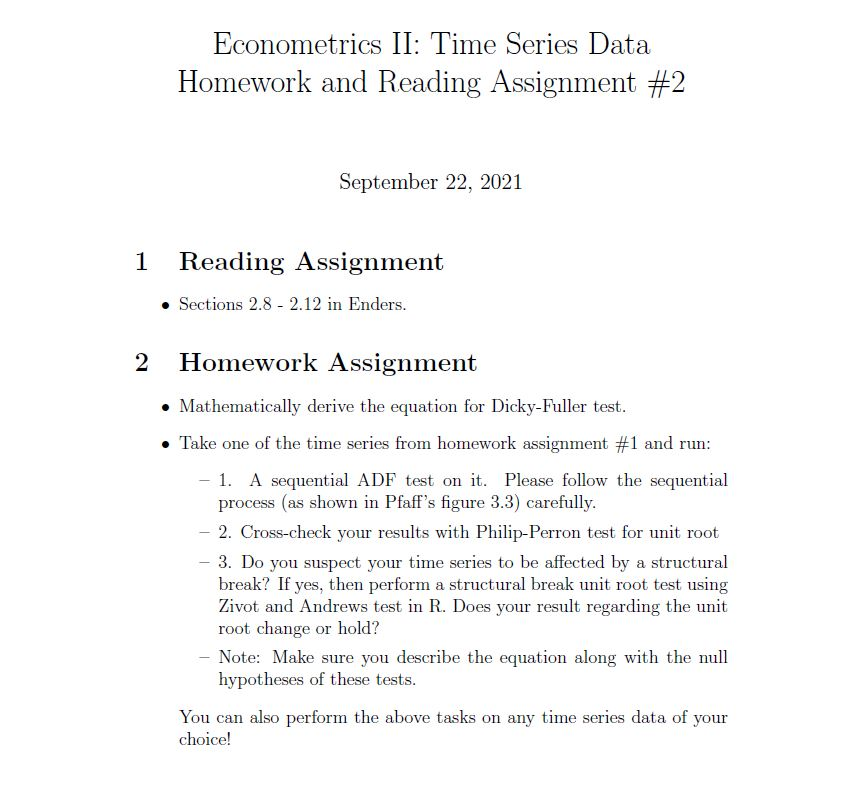
\includegraphics{Eksamen2.jpg} \newpage

\hypertarget{mathematically-derive-the-equation-for-dicky-fuller-test.}{%
\subsection{Mathematically derive the equation for Dicky-Fuller
test.}\label{mathematically-derive-the-equation-for-dicky-fuller-test.}}

Vi starter med at opskrive en variable \(Y_t\) på en AR(1) process\\
\[Y_t = \theta Y_{t-1} + \epsilon_t\] Så trækkes \(Y_{t-1}\) fra på
begge sider \[ Y_{t} - Y_{t-1}=\theta Y_{t-1}-Y_{t-1}+\epsilon_{t} \] Vi
trækker den nutidige værdi fra den tidligere værdi for at få
\(\Delta Y_t\), og \(Y_t\) sættes uden for parantes
\[\Delta Y_t=(\theta-1)Y_{t-1}+\epsilon_t    \] Vi kalder \((\theta-1)\)
for \(\pi\) for at generalisere.
\[\Delta Y_t=\pi Y_{t-1} + \epsilon_t    \]

Hvor vi antager at \(\epsilon\) følger en white noise process.\\
\[\epsilon \sim IID(0,\sigma^2)\]\\
Der gælder forskellige ting for \(\theta\) :\\
Hvis \(|\theta|\) \(<\) 1 så er det en stationær process\\
Hvis \(|\theta|\) = 1 så er der unit root i tidsserien, og processen er
ikke stationær\\
Hvis \(|\theta|\) \(>\) 1 så eksplodere processen\\
~\\
Når vi laver en unit root test, så bruger vi\\
\textbf{Nulhypotesen}: \[H_0: \theta = 1 \tag{Unit root} \]
\textbf{Alternative hypotese}: \[H_1: \theta < 1 \tag{No unit root}\]

Grunden til vi tester om theta er mindre end 1 er, at det kun er der
hvor det er en stationær process. Vi kan altså ikke bruge den
alternative hypotese at theta er forskellige fra 1.\\
Efter omskriv så kan vi opskrive vores hypoteser på følgende måde\\
\textbf{Nulhypose}: \[H_0: \pi = 0 \tag{Unit root}\]
\textbf{Alternative hypotese} \[H_1: \pi < 0 \tag{No unit root}\]

Der gælder for Dickey-Fuller testen at hvis \(\pi = 0\) så er
\(\theta = 1\), og det betyder at der er unit root i vores tidsserie. Vi
skal ikke bruge vores almindelige t-værdier, men derimod sammenligne dem
med DF(tau)-statistikkerne som kan ses i appendix.

\hypertarget{a-sequential-adf-test-on-it.-please-follow-the-sequential-process-as-shown-in-pfaffs-figure-3.3-carefully.}{%
\subsubsection{A sequential ADF test on it. Please follow the sequential
process (as shown in Pfaff's figure 3.3)
carefully.}\label{a-sequential-adf-test-on-it.-please-follow-the-sequential-process-as-shown-in-pfaffs-figure-3.3-carefully.}}

I denne opgave bruger vi BNP, som vi også har brugt tidligere.

Her skal vi først teste vores data for unit root. Dette gøres fordi, at
unit root kan give problemer i ens modeller, da det gør det sværere at
forudsige fremtidige bevægelser. Unit root er en tilfældig trend i en
tidsserie, som også bliver kaldt ``random walk with drift''.\\
~\\
En ADF-test er blot en videreudvikling af DF-testen, og tester også for
unit root i ens data. Hvis T-værdierne fra ADF er mindre end tau
værdierne, så kan man forkaste \(H_0\).\\
~\\

Opstiller hypoteser\\
\textbf{Nulhypotesen}:\\
\[H_0: \pi = 0 \tag{Unit root}  \] \textbf{Den alternative hypotese}:\\
\[H_1: \pi < 0 \tag{No unit root} \]

Estimerer vores regressioner:
\[\Delta Y_t = \delta Y_{t-1}  + \epsilon_t \tag{No intercept, no trend}  \]
\[\Delta Y_t = \alpha +  \delta Y_{t-1}  + \epsilon_t \tag{Intercept, no trend}  \]
\[\Delta Y_t = \alpha+ \beta t + \delta Y_{t-1}  + \epsilon_t \tag{Intercept, trend}  \]

\begin{longtable}[]{@{}lrrrr@{}}
\caption{Regression uden intercept og trend}\tabularnewline
\toprule
& Estimate & Std. Error & t value &
Pr(\textgreater\textbar t\textbar)\tabularnewline
\midrule
\endfirsthead
\toprule
& Estimate & Std. Error & t value &
Pr(\textgreater\textbar t\textbar)\tabularnewline
\midrule
\endhead
L(BNP\_ts, 1) & 0.0032937 & 0.0024327 & 1.353927 &
0.1768878\tabularnewline
\bottomrule
\end{longtable}

\textbf{Når T < Tau, så kan vi forkaste $H_0$}\\
\textbf{Når T > tau, så kan vi ikke forkaste $H_0$}

Her kan vi se, at pga. vores T værdi større end -1.95(jf. appendix) på
et 5\% sigfikansniveau, kan vi ikke afvise vores nulhypotese. Det tyder
derfor på, at der er unit root i vores regression uden intercept og uden
trend.

\newpage

\begin{longtable}[]{@{}lrrrr@{}}
\caption{Regression med intercept uden trend}\tabularnewline
\toprule
& Estimate & Std. Error & t value &
Pr(\textgreater\textbar t\textbar)\tabularnewline
\midrule
\endfirsthead
\toprule
& Estimate & Std. Error & t value &
Pr(\textgreater\textbar t\textbar)\tabularnewline
\midrule
\endhead
(Intercept) & 2606.9064523 & 1620.6080890 & 1.6085977 &
0.1088730\tabularnewline
L(BNP\_ts, 1) & -0.0059439 & 0.0062339 & -0.9534896 &
0.3411949\tabularnewline
\bottomrule
\end{longtable}

\textbf{Når T < Tau, så kan vi forkaste $H_0$}\\
\textbf{Når T > tau, så kan vi ikke forkaste $H_0$}

Her kan vi se, at vi stadigvæk ikke kan afvise nulhypotesen, da vores
T-værdi stadigvæk er større end vores tau værdi -2.89 på et 5\%
signifikansniveau.

\begin{longtable}[]{@{}lrrrr@{}}
\caption{Regression med intercept og trend}\tabularnewline
\toprule
& Estimate & Std. Error & t value &
Pr(\textgreater\textbar t\textbar)\tabularnewline
\midrule
\endfirsthead
\toprule
& Estimate & Std. Error & t value &
Pr(\textgreater\textbar t\textbar)\tabularnewline
\midrule
\endhead
(Intercept) & 25881.2431844 & 3321.8685952 & 7.791170 & 0\tabularnewline
L(BNP\_ts, 1) & -0.3788454 & 0.0480916 & -7.877578 & 0\tabularnewline
trend(diff(BNP\_ts)) & 1934.9044044 & 247.8154911 & 7.807843 &
0\tabularnewline
\bottomrule
\end{longtable}

\textbf{Når T < Tau, så kan vi forkaste $H_0$}\\
\textbf{Når T > tau, så kan vi ikke forkaste $H_0$}

Her har vi en T-værdi, der er mindre end vores tau-værdi -3.45 Derfor
kan nulhypotesen afvises på et 5\% signifikansniveau, og det tyder på,
at der i regressionen med intercept og trend, ikke er unit root.\\

Så gør vi det samme, men nu med \(\Delta BNP\). Opstiller hypoteser\\
\textbf{Nulhypotesen}\\
\[ H_0: \pi = 0 \tag{Unit root} \] \textbf{Den alternative hypotese}\\
\[H_1: \pi < 0 \tag{No unit root} \]

\newpage

Plotter først vores data for at se, om det ser stationært ud:

\begin{figure}[H]

{\centering \includegraphics[width=0.9\linewidth]{figures/unnamed-chunk-22-1} 

}

\caption{\label{fig:bnpdiff}Plot af DeltaBNP}\label{fig:unnamed-chunk-22}
\end{figure}

I figur \ref{fig:bnpdiff} kan vi se, at vores data har nogle få store
udsving, men at det ellers ser rimelig stationært ud. Dog tester vi
yderligere ved hjælp af regressioner, ligesom vi gjorde tidligere.

\begin{longtable}[]{@{}lrrrr@{}}
\caption{DeltaBNP-Regression uden intercept og trend}\tabularnewline
\toprule
& Estimate & Std. Error & t value &
Pr(\textgreater\textbar t\textbar)\tabularnewline
\midrule
\endfirsthead
\toprule
& Estimate & Std. Error & t value &
Pr(\textgreater\textbar t\textbar)\tabularnewline
\midrule
\endhead
L(BNP\_d, 1) & -1.697383 & 0.0442467 & -38.36178 & 0\tabularnewline
\bottomrule
\end{longtable}

Her kan vi afvise nulhypotesen, fordi T-værdien er mindre end
tau-værdien. Det tyder derfor ikke på, at der er unit root i vores
første difference af BNP uden intercept og trend.

\begin{longtable}[]{@{}lrrrr@{}}
\caption{DeltaBNP-Regression med intercept uden trend}\tabularnewline
\toprule
& Estimate & Std. Error & t value &
Pr(\textgreater\textbar t\textbar)\tabularnewline
\midrule
\endfirsthead
\toprule
& Estimate & Std. Error & t value &
Pr(\textgreater\textbar t\textbar)\tabularnewline
\midrule
\endhead
(Intercept) & 2081.148555 & 445.9826255 & 4.666434 &
4.8e-06\tabularnewline
L(BNP\_d, 1) & -1.721867 & 0.0429583 & -40.082236 &
0.0e+00\tabularnewline
\bottomrule
\end{longtable}

Igen kan vi kigge på væres T-værdier og afvise unit root i første
difference af BNP med intercept uden trend.

\begin{longtable}[]{@{}lrrrr@{}}
\caption{DeltaBNP-Regression med intercept og trend}\tabularnewline
\toprule
& Estimate & Std. Error & t value &
Pr(\textgreater\textbar t\textbar)\tabularnewline
\midrule
\endfirsthead
\toprule
& Estimate & Std. Error & t value &
Pr(\textgreater\textbar t\textbar)\tabularnewline
\midrule
\endhead
(Intercept) & 2069.2803868 & 895.6673205 & 2.3103225 &
0.0216301\tabularnewline
L(BNP\_d, 1) & -1.7218712 & 0.0430394 & -40.0068239 &
0.0000000\tabularnewline
trend(BNP\_d) & 0.3466849 & 22.6755436 & 0.0152889 &
0.9878130\tabularnewline
\bottomrule
\end{longtable}

Til sidst kan vi afvise unit root i første difference af BNP med trend
og intercept. Dog tyder det på, at der er både trend og intercept i
vores data, da disse værdier ikke kan afvises på et 5\% signifikans
niveau jf. vores tau-værdi fra appendix: \(-3.45\)\\

Ved at tage første difference og tilføje trend og intercept, har vi
fjernet alt unit root i BNP, og vi kan derfor kalde BNP for en
I(1)-process.

\hypertarget{cross-check-your-results-with-philip-perron-test-for-unit-root}{%
\subsubsection{Cross-check your results with Philip-Perron test for unit
root}\label{cross-check-your-results-with-philip-perron-test-for-unit-root}}

Da vi gerne vil krydstjekke vores resultater fra tidligere, kan vi bruge
Philip-Perron testen. I \({\rm I\!R}\) er
\textbf{nulhypotesen for PP testen givet ved:}
\[H_0: \theta = 1 \tag{Unit root} \] \textbf{Alternative hypotese:}
\[H_1: \theta < 1 \tag{No unit root} \] Det betyder at hvis vi kan
afvise \(H_0\) så er der IKKE unit root i vores tidsserie, og hvis vi
IKKE kan forkaste \(H_0\) så kan der være unit root i vores tidsserie i
levels.

\begin{longtable}[]{@{}rl@{}}
\caption{PP-test for BNP og DeltaBNP}\tabularnewline
\toprule
pvalue & Variabel\tabularnewline
\midrule
\endfirsthead
\toprule
pvalue & Variabel\tabularnewline
\midrule
\endhead
0.01 & BNP\_ts\tabularnewline
0.01 & BNP\_d\tabularnewline
\bottomrule
\end{longtable}

Da vi får en p-værdi på 0.01 for begge, kan vi forkaste på en 5\%
siknifikansniveau, at det skulle være unit root i vores data. Vores data
er altså stationært. Vi ved at PP-testen medtager intercept og trend, og
vores resultater hænger derfor sammen med ADF-testen, som vi kørte
tidligere.

\hypertarget{do-you-suspect-your-time-series-to-be-affected-by-a-structural-break-if-yes-then-perform-a-structural-break-unit-root-test-using-zivot-and-andrews-test-in-r.-does-your-result-regarding-the-unit-root-change-or-hold}{%
\subsubsection{Do you suspect your time series to be affected by a
structural break? If yes, then perform a structural break unit root test
using Zivot and Andrews test in R. Does your result regarding the unit
root change or
hold?}\label{do-you-suspect-your-time-series-to-be-affected-by-a-structural-break-if-yes-then-perform-a-structural-break-unit-root-test-using-zivot-and-andrews-test-in-r.-does-your-result-regarding-the-unit-root-change-or-hold}}

Et strukturelt brud er når tidsserien ikke befinder sig omkring samme
gennemsnit gennem hele serien. Så hvis der fx. er et stort spring/stød
et sted i tidsserien, kan det give mening at teste de to forskellige
``perioder'' med hver deres gennemsnit. I denne test bruger vi både
intercept og trend, da vi tidligere har fundet, at dette var mest
optimalt for vores tidsserie.

za-testen giver ``En potentiel break position'' ved observation nr. 118.

Ligesom ved det almindelige plot kan vi se, at der er et potentielt
break omkring kvartal (år 1979, 2. kvartal). Det kan faktisk også ses et
break omkring finanskrisen, men za-testen kan kun finde ét breakpoint.\\

Vi får en T-statistik på -4.6565, hvor den kritiske værdi for et 10\%
signifikansniveau er -4.82. Vi kan altså på et 10\% signifikansniveau
afvise unit root i vores data. Så vi kan godt have en stationær process,
selvom der er strukturelle breaks i vores tidsserie.

\begin{figure}[H]

{\centering \includegraphics[width=0.9\linewidth]{figures/unnamed-chunk-29-1} 

}

\caption{\label{fig:bnpbreak}Plot af potentiel break i vores tidsserie}\label{fig:unnamed-chunk-29}
\end{figure}

Her kan vi ved den blå linje se, at der sker en skift i gennemsnittet
for vores data. Det får altså et stød nedad og forbliver nede i det
``niveau''. Det er derfor et strukturel break.

\newpage

\hypertarget{eksamensopgave-3}{%
\section{Eksamensopgave 3}\label{eksamensopgave-3}}

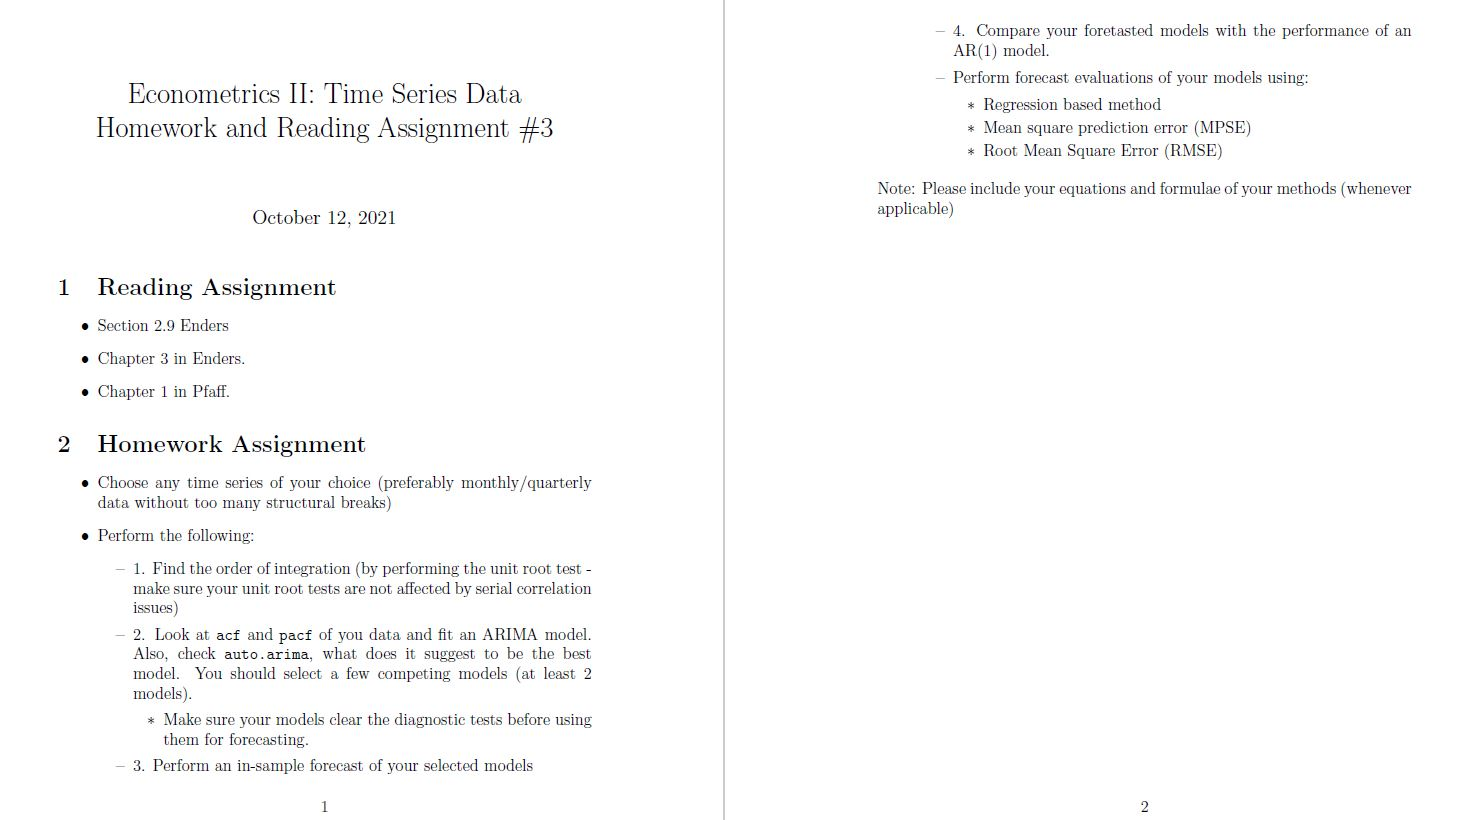
\includegraphics{Eksamen3.jpg} \newpage

\hypertarget{chose-any-timeseries-of-your-choice}{%
\subsection{Chose any timeseries of your
choice:}\label{chose-any-timeseries-of-your-choice}}

Vi vælger igen BNP\_ts, som vi også brugte i Eksamenssæt 2.

\hypertarget{find-the-order-of-integration-by-performing-the-unit-root-test---make-sure-your-unit-root-tests-are-not-afected-by-serial-correlation-issues}{%
\subsection{1. Find the order of integration (by performing the unit
root test - make sure your unit root tests are not afected by serial
correlation
issues)}\label{find-the-order-of-integration-by-performing-the-unit-root-test---make-sure-your-unit-root-tests-are-not-afected-by-serial-correlation-issues}}

\hypertarget{inspektion-af-data}{%
\subsubsection{Inspektion af data}\label{inspektion-af-data}}

Først kan vi lave en inspektion af vores data for at se, hvordan det ser
ud. Om det ser ud til, at der kunne være seasonality, unit root,
struktural breaks eller måske en opadgående trend.

\begin{figure}[H]

{\centering \includegraphics[width=0.9\linewidth]{figures/unnamed-chunk-30-1} 

}

\caption{\label{fig:bnpbreak2}Plot af potentiel break i vores tidsserie}\label{fig:unnamed-chunk-30}
\end{figure}

Her kan vi se, at der måske er en trend, og måske et struktural break
omkring 1979.\\
~\\

\hypertarget{seasonality-og-trend}{%
\paragraph{Seasonality og trend}\label{seasonality-og-trend}}

\leavevmode

Inden vi laver unit root tests, vil vi først teste for seasonality, så
vi er sikre på, at dette ikke er til stede. Dette gøres ved at bruge
dummy-variabel metoden:
\[BNP_t = \alpha+\beta_2D_2+\beta_3D_3+\beta_4D_4+\epsilon_t\]
\textbf{Nulhypotese} \[
H_0 : \beta_2 = \beta_3 = \beta_4 = 0 
\tag{No seasonality} \] \textbf{Alternativ hypotese} \[
H_1 : \beta_2 \neq \beta_3 \neq \beta_4 \neq 0 
\tag{Seasonality} \]

F-testen går ind og bruger dummy variablerne ved at sætte et enkelt
kvartal til at være 1, fx. \(D_2=1\), og sætter de resterende til at
være 0. Det betyder at der kun fåes data fra et bestemt kvartal i
regressionen, og man kigger derfor på kvartalerne individuelt istedet
for at kigge på den samlede tidsserie. Man kan derfor finde ud af om
kvartalerne i sig selv er signifikante eller ej. Hvis de er
signifikante, så vil der være seasonality i det pågældende kvartal.

\begin{table}[!htbp] \centering 
  \caption{} 
  \label{} 
\begin{tabular}{@{\extracolsep{5pt}}lc} 
\\[-1.8ex]\hline 
\hline \\[-1.8ex] 
 & \multicolumn{1}{c}{\textit{Dependent variable:}} \\ 
\cline{2-2} 
\\[-1.8ex] & BNP\_ts \\ 
\hline \\[-1.8ex] 
 q1 & $-$8,861.918 (17,443.130) \\ 
  q2 & $-$3,495.046 (17,506.670) \\ 
  q3 & $-$9,262.135 (17,506.670) \\ 
  Constant & 245,469.000$^{***}$ (12,379.090) \\ 
 \hline \\[-1.8ex] 
Observations & 273 \\ 
R$^{2}$ & 0.001 \\ 
Adjusted R$^{2}$ & $-$0.010 \\ 
Residual Std. Error & 102,080.600 (df = 269) \\ 
F Statistic & 0.130 (df = 3; 269) \\ 
\hline 
\hline \\[-1.8ex] 
\textit{Note:}  & \multicolumn{1}{r}{$^{*}$p$<$0.1; $^{**}$p$<$0.05; $^{***}$p$<$0.01} \\ 
\end{tabular} 
\end{table}

I tabellen kan man først se estimaterne, derefter kan standardafvigelsen
ses i parantesen og til sidst kan man se ``p-værdierne'' opløftet i
stjerner. Der er ikke nogle siknifikante P-værdi, så vi kan afvise
nulhypotesen. Dette tyder på, at der ikke er seasonality i vores data.

Nu vil vi gerne se, om der er en trend i vores data. Dette gøres ved at
plotte residualerne.

\begin{figure}[H]

{\centering \includegraphics[width=0.9\linewidth]{figures/unnamed-chunk-33-1} 

}

\caption{\label{fig:bnpbreak}Plot af residualer}\label{fig:unnamed-chunk-33}
\end{figure}

Det ligner der er en klar opadgående trend, og at residualerne ikke
flukturere omkring en bestemt middelværdi.

\newpage

\hypertarget{unit-root-tests}{%
\subsubsection{Unit root tests}\label{unit-root-tests}}

Da vores tiddsserie har tegn på en trend kan vi nu teste for unit root
med en tidsserie, der indeholder en trend. Dog vælger vi alligevel at
undersøge alle muligheder end blot med trend, så vi undersøger:\\
\[\Delta Y_t = \delta Y_{t-1}  + \epsilon_t \tag{No intercept, no trend}  \]
\[\Delta Y_t = \alpha +  \delta Y_{t-1}  + \epsilon_t \tag{Intercept, no trend}  \]
\[\Delta Y_t = \alpha+ \beta t + \delta Y_{t-1}  + \epsilon_t \tag{Intercept, trend}  \]

Så vil vi bruge ADF-testen til at teste for unit root.\\
Her skal vi bruge tau-værdierne til at vurdere, om vi har unit roots
eller ej, så først opstiller vi vores nulhypoteser:\\
\textbf{Nulhypotesen}:\\
\[H_0: \pi = 0 \tag{Unit root}  \] \textbf{Den alternative hypotese}:\\
\[H_1: \pi < 0 \tag{No unit root} \] Hvis T-værdierne fra ADF er mindre
end tau værdierne, så kan man forkaste \(H_0\).\\
Hvis T-værdier fra ADF er større end tau værdierne, så kan vi
\textbf{IKKE} forkaste \(H_0\)

Vi udfører først testen på følgende vis:\\
- Uden trend og drift.\\
- Uden trend og med drift.\\
- Med trend og med drift.\\

\begin{longtable}[]{@{}lrrr@{}}
\caption{ADF-test for BNP-modeller}\tabularnewline
\toprule
& none & drift & trend\tabularnewline
\midrule
\endfirsthead
\toprule
& none & drift & trend\tabularnewline
\midrule
\endhead
Unit root & 4.134608 & -0.3285513 & -3.291536\tabularnewline
drift & & 10.9056709 & 11.108403\tabularnewline
trend & & & 5.417225\tabularnewline
\bottomrule
\end{longtable}

Her får vi en masse forskellige værdier, så skal sammenlignes med
tau-værdierne, man kan få fra cval i selve adf-testen.\\
~\\
\textbf{Når T < Tau, så kan vi forkaste $H_0$}\\
\textbf{Når T > tau, så kan vi ikke forkaste $H_0$}

\begin{longtable}[]{@{}lrrr@{}}
\caption{Tau værdier for ADF-testen på 5\%
signifikansniveau}\tabularnewline
\toprule
& none & drift & trend\tabularnewline
\midrule
\endfirsthead
\toprule
& none & drift & trend\tabularnewline
\midrule
\endhead
Unit root & -1.95 & -2.87 & -3.42\tabularnewline
drift & & 4.61 & 4.71\tabularnewline
trend & & & 6.30\tabularnewline
\bottomrule
\end{longtable}

De oprindelige tau-værdier kan godt være svære at forholde sig til, da
de kommer i mange forskellige signifikansniveauer og hypoteserne ikke er
klare. Derfor har vi fundet en pakke på
\href{https://www.r-bloggers.com/2021/12/easy-interpretations-of-adf-test-in-r/}{R-bloggers}
, som opstiller det hele for os.

\begin{verbatim}
## ========================================================================
## At the 5pct level:
## The model is of type none
## tau1: The null hypothesis is not rejected, unit root is present
## ========================================================================
## ========================================================================
## At the 5pct level:
## The model is of type drift
## tau2: The first null hypothesis is not rejected, unit root is present
## phi1: The second null hypothesis is rejected, unit root is present
##       and there is drift.
## ========================================================================
## ========================================================================
## At the 5pct level:
## The model is of type trend
## tau3: The first null hypothesis is not rejected, unit root is present
## phi3: The second null hypothesis is not rejected, unit root is present
##       and there is no trend
## phi2: The third null hypothesis is rejected, unit root is present
##       there is no trend, and there is drift
## ========================================================================
\end{verbatim}

Da vi har unit root i levels, så kigger vi først, om det kan skyldes
seriekorrelation, men ellers går vi videre til at tage first difference.

\newpage

\hypertarget{seriekorrelation}{%
\subsubsection{Seriekorrelation}\label{seriekorrelation}}

Vi tester nu om vores unit root skyldes seriekorrelation. Vi tester
efter seriekorrelation med Ljungs-box for at se, om det er
seriekorrelation, der er problemet.

\begin{center}\includegraphics[width=0.9\linewidth]{figures/unnamed-chunk-40-1} \end{center}

Vi kan som ovenfor også se, at der op til 7 lags er seriekorrelation,
men at denne forsvinder ved lag 7.\\
Lagsne kan fjernes manuelt for at eliminere unit root, eller man kan
tage første difference og få en I(1) process, og måske eliminere unit
root på den måde. Vi vælger selv at tage forskellen og få en I(1)
process så: \[\Delta y = y_t-y_{t-1} \] Derefter tester vi igen for unit
root med Philips-Perron testen.

Her får vi en p-værdi på 0.01, og vi kan derfor afvise på et 5\%
signifikansniveau, at der skulle være unit root i vores tidsserie. Vi
har altså fjernet unit root i vores data ved en I(1)-process.
Konklusionen er dermed, at vores BNP data er en I(1)-process

\newpage

\hypertarget{look-at-acf-and-pacf-of-you-data-and-fit-an-arima-model.}{%
\subsection{2. Look at acf and pacf of you data and fit an ARIMA
model.}\label{look-at-acf-and-pacf-of-you-data-and-fit-an-arima-model.}}

Man kan bruge ACF og PACF til at undersøge hvilken type model, der kan
være et godt match til ens tidsserie. De kan ikke 100\% fortælle hvilken
rigtig model, man skal anvende, men de er gode pejlemærker og fungerer
godt sammen med yderligere analyse.\\
~\\
Plotter for vores I(1)-process(yd), da vi skal bruge stationært data i
vores model, da det ikke giver mening at forecaste med ustabilt data. Da
vi arbejder med kvartalsvis data, er der 4 lags på et år.

\begin{center}\includegraphics[width=0.9\linewidth]{figures/unnamed-chunk-43-1} \end{center}

\textbf{ACF}\\
ACF fortæller noget om variablen og dets egne laggede værdier. Kigger vi
på grafen kan vi se, at den aftager over tid og lagsne skifter i
signifikans. Dette kunne tyde på, at vi har MA(2)-process.

\newpage

\textbf{PACF}\\
PACF tester for en serie af lags i tidsserien. Og den tester derfor på
tværs af flere lags end ACF. Kigger vi på grafen ovenfor, kan vi se, at
der er en stærk korrelation i andet kvartal. Derudover er mange af
lagsne ikke signifikante. Dette kunne tyde på en AR(2)-process.\\

Sammenholder man de to grafer vil det tyde på, at vi har at gøre med en
ARIMA(2,1,2) process, men vi kan teste dette bedre ved hjælp af
\({\rm I\!R}\), frem for visuel inspektion.\\
Dette kan gøres med auto.arima, som finder den optimale model for
tidsserien.

Her får vi givet ARIMA(1,1,1)(2,1,2) som den bedste model. Den vil vi nu
teste om er stationær ved hjælp af unit root cirklen.

\begin{center}\includegraphics[width=0.9\linewidth]{figures/unnamed-chunk-45-1} \end{center}

Da alle de inverse rødder af AR og MA er indenfor unit root cirklen, så
er ARIMA modellen stationær, og vi kan derfor bruge den til at forecaste
med senere. Generelt set viser unit root cirklen som regel kun dem, som
falder inden for cirklen, men vi kan også simulere et scenarie, hvor de
falder udenfor. Dette gøres i appendix.

\newpage

\hypertarget{robusthedstest}{%
\subsubsection{Robusthedstest}\label{robusthedstest}}

For at være sikre på, at vores resultater er korrekte, kører vi en
robusthedstest:.

\begin{center}\includegraphics[width=0.9\linewidth]{figures/unnamed-chunk-46-1} \end{center}

Her kan vi se, at residualerne svinger omkring middelværdien (0-linjen),
Vores ACF ser ud som den skal med undtaget af et enkelt lag(2.25 ca) og
vores Ljung box viser ikke tegn på seriekorrelation.\\

\hypertarget{normality}{%
\paragraph{Normality}\label{normality}}

\leavevmode

Næst vil teste om residualerne er normalfordelte. Dette gøres igennem
Jarque-Bera-testen, hvor hypoteserne kan opstilles:\\
\textbf{Nulhypotese:}
\[ H_0:\epsilon \sim N(0,\sigma^2) \tag{Residualer er normalfordelte}   \]
\textbf{Alternativ hypotese:}
\[ H_1:\epsilon \neq N(0,\sigma^2) \tag{Residualerne er ikke normalfordelte} \]
Her får vi en p-værdi på 0.1205, så vi kan ikke forkaste nulhypotesen på
et 5\% signifikansniveau. Det vil altså sige, at vores residualer ser ud
til at være normalfordelte. Hvis residualerne ikke er normalfordelte,
bliver vi nødt til at lave flere tests med fx. dummy variable, kigge på
strukturel breaks eller lignende.

\hypertarget{lagshar-vi-rette-antal-lags-med}{%
\paragraph{Lags(Har vi rette antal lags
med)}\label{lagshar-vi-rette-antal-lags-med}}

\leavevmode

Derefter kan vi teste om vi har den korrekte mængde lags med i modellen.
Dette gøres ved at teste vores ARIMA model. Her får vi, at vi har de
rette AR og MA lags. Dette giver også bedst mening, da vi har brugt
auto.arima funktionen, som finder ud af dette automatisk.

\hypertarget{arch}{%
\paragraph{ARCH}\label{arch}}

\leavevmode

Derefter tester vi for hetereoskedascicitet i vores model. Dette vil man
ikke have i modellen, da det leder til ineffektive standard errors og
skaber seriekorrelation i fejlledet. Dette kan vi teste for ved hjælp af
ARCH-testen. \[ H_0 : No \ autocorrelation / no \ heteroskedacity\]
\[ H_1 : Autocorrelation / heteroskedacity\]

Så laver vi ARCH-testen

\begin{center}\includegraphics[width=0.9\linewidth]{figures/unnamed-chunk-49-1} \end{center}

Vi kan på figuren se, at vi ikke kan forkaste \(H_0\). Dette betyder, at
vi ikke har autokorrelation i vores model. Vi bryder derfor ikke TS4
omhandlende homoskedascitet. Jf. appendix.\\
Vi har nu testet vores data og konkluderer, at det godt kan bruges til
forecasting i de næste opgaver.

\newpage

\hypertarget{perform-an-in-sample-forecast-of-your-selected-models}{%
\subsection{3. Perform an in-sample forecast of your selected
models}\label{perform-an-in-sample-forecast-of-your-selected-models}}

Vi vælger at tage de to bedste og de to dårligste modeller at forecaste
for, at man kan se en klar forskel i hvorfor man skal vælge de rigtige
modeller:

\begin{figure}[H]

{\centering \includegraphics[width=0.9\linewidth]{figures/unnamed-chunk-50-1} 

}

\caption{\label{fig:forecastplot}Plot af forecasts}\label{fig:unnamed-chunk-50}
\end{figure}

Her kan vi se, at den øverste til venstre, er den bedste model, men den
nederste til venstre er den dårligste model. Den øverste til højre, er
den næstbedste, mens den nederste til højre er den næstdårligste model.
Det kan vi bla. se på konfidensintervallerne(de blå skygger), hvor et
højere konfidensinterval betyder større usikkerhed i modellen.

\newpage

\hypertarget{compare-your-foretasted-models-with-the-performance-of-an-ar1-model.}{%
\subsection{4. Compare your foretasted models with the performance of an
AR(1)
model.}\label{compare-your-foretasted-models-with-the-performance-of-an-ar1-model.}}

En AR(1) er det samme som en ARIMA(1,0,0) og er ikke en særlig god måde
at forecaste på. Dette kan vi se i plottet.

\begin{figure}[H]

{\centering \includegraphics[width=0.9\linewidth]{figures/unnamed-chunk-51-1} 

}

\caption{\label{fig:AR1}Plot af AR(1)}\label{fig:unnamed-chunk-51}
\end{figure}

Selv vores dårligste ARIMA modeller er bedre end vores AR(1) model. AR
modellen kan kun forudsige linært.

\hypertarget{perform-forecast-evaluations-of-your-models-using}{%
\subsection{5. Perform forecast evaluations of your models
using:}\label{perform-forecast-evaluations-of-your-models-using}}

Der er forskellige måder at evaluere sine forecasts på. Nogle af dem vil
vi gennemgå i dette afsnit.

\hypertarget{regression-based-method}{%
\subsubsection{Regression based method:}\label{regression-based-method}}

Nu laver vi en regression af det realle data på det forecastede data.
Regressionen kan ses nedenfor:
\[\underbrace{{{[Y_a]}}_{263}^{272}}_\text{reelle data} = \alpha_A + \beta_A \underbrace{ [\hat{Y}_A]_{263}^{272}}_\text{forecastede data} + [\epsilon]_{1}^{9}  \]\\
Vi kan nu opstille hypoteserne vi skal teste.\\
\textbf{Nulhypotesen}:
\[H_0: \alpha_A = 0 \ og\ \beta_A = 1 \tag{Ikke Forecast bias} \]
\textbf{Alternativ hypotese}:
\[H_1: \alpha_A \neq 0 \ og \ \beta_A \neq 1 \tag{Forecast bias} \]

Vi tester altså hvor godt det forecastede in-sample data passer på det
reelle data. Dette kaldes også forecast bias.

\begin{longtable}[]{@{}lrr@{}}
\caption{Test for forecast bias i vores modeller}\tabularnewline
\toprule
Model & Pvalue & RSS\tabularnewline
\midrule
\endfirsthead
\toprule
Model & Pvalue & RSS\tabularnewline
\midrule
\endhead
Bedste & 0.437 & 283462839\tabularnewline
Næst Bedst & 0.479 & 277429211\tabularnewline
Dårligste & 0.001 & 291300020\tabularnewline
Næst Dårligst & 0.001 & 245415408\tabularnewline
\bottomrule
\end{longtable}

Ved den bedste og næst bedste model kan vi ikke afvise nulhypotesen, da
vi har en høj p-værdi. Dette betyder, at modellerne ikke viser tegn på
forecast bias. Ved den dårligste og næst dårligste model kan vi
tilgengæld godt afvise nulhypotesen, da vi har en lav p-værdi. Dette
tyder på, at der i de to dårligste modeller, er forecast bias. Når man
har to modeller, hvor man ikke kan afvise forecast bias, så skal man
vælge den med lavest RSS(Residual standard error). Det tyder faktisk på,
at dette er vores ``næst-bedste'' model.

\hypertarget{mean-square-prediction-error-mpse}{%
\subsubsection{Mean square prediction error
(MPSE)}\label{mean-square-prediction-error-mpse}}

Her bruger vi gennemsnittet fra de forecastede modeller.

Her bruger vi den bedste, næst-bedste, næst-dårligste, dårligste og til
sidst vores AR model.

\begin{longtable}[]{@{}lrrrrr@{}}
\caption{Tabel med MPSE for vores udvalgte modeller}\tabularnewline
\toprule
& Bedste & Næst-Bedst & Dårligste & Næst-Dårligst &
AR-model\tabularnewline
\midrule
\endfirsthead
\toprule
& Bedste & Næst-Bedst & Dårligste & Næst-Dårligst &
AR-model\tabularnewline
\midrule
\endhead
MPSE & 16328244 & 11417411 & 753203433 & 725807117 &
232311195\tabularnewline
\bottomrule
\end{longtable}

Her kan vi se, at MPSE faktisk er lavest ved den næstebedste model.
Dette tyder på, at vores bedste model måske ikke er den bedste
alligevel, som vi også opdagede i forrige opgave.

\hypertarget{root-mean-square-error-rmse}{%
\subsubsection{Root Mean Square Error
(RMSE)}\label{root-mean-square-error-rmse}}

\begin{longtable}[]{@{}lrrrrr@{}}
\caption{Tabel med RMSE for vores udvalgte modeller}\tabularnewline
\toprule
& Bedste & Næst-Bedst & Dårligste & Næst-Dårligst &
AR-model\tabularnewline
\midrule
\endfirsthead
\toprule
& Bedste & Næst-Bedst & Dårligste & Næst-Dårligst &
AR-model\tabularnewline
\midrule
\endhead
RMSE & 4040.822 & 3378.966 & 27444.55 & 26940.81 &
15241.76\tabularnewline
\bottomrule
\end{longtable}

Her bruger vi den bedste, næst-bedste, næst-dårligste, dårligste og til
sidst vores AR model. Her ser vi samme tendens som ved MPSE. Den
næstbedste model er stadigvæk den bedste ift. RMSE, og det kunne tyde
på, at auto.arima måske ikke har valgt den bedste model.

\newpage

\hypertarget{eksamensopgave-4}{%
\section{Eksamensopgave 4}\label{eksamensopgave-4}}

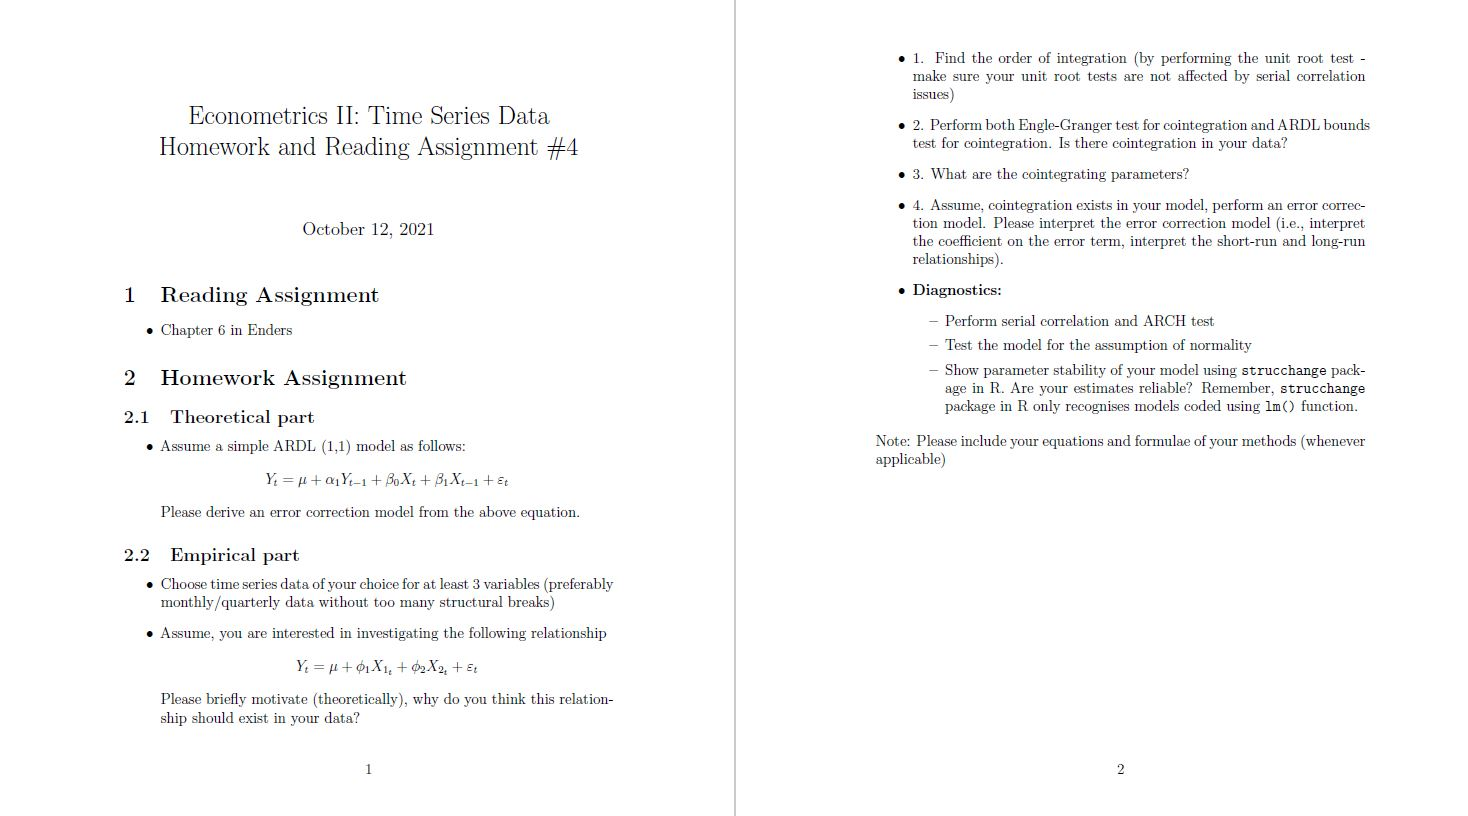
\includegraphics{Eksamen4.jpg} \newpage

\hypertarget{theoretical-part}{%
\subsection{Theoretical part}\label{theoretical-part}}

\hypertarget{assume-a-simple-ardl-11-model-as-follows}{%
\subsubsection{Assume a simple ARDL (1,1) model as
follows:}\label{assume-a-simple-ardl-11-model-as-follows}}

\[Y_t = \mu + \alpha_1Y_{t-1} + \beta_0X_t + \beta_1X_{t-1} + \epsilon_t \]

\textbf{Please derive an error correction model from the above equation}:\\
Vi starter med at trække \(Y_{t-1}\) fra på begge sider
\[Y_t - Y_{t-1} = \mu + \alpha_1Y_{t-1}- Y_{t-1} + \beta_0X_t + \beta_1X_{t-1} + \epsilon_t \]
Vi får forskellen på \(Y_t\) på venstreside, hvor vi på højreside der
kan vi tage \(Y_{t-1}\) udenfor parantes
\[\Delta Y_t = \mu - (1 - \alpha_1)Y_{t-1} + \beta_0X_t + \beta_1X_{t-1} + \epsilon_t \]
Vi trækker nu \(\beta_0X_{t-1}\) fra på begge sider
\[\Delta Y_t - \beta_0X_{t-1} = \mu - (1 - \alpha_1)Y_{t-1} + \beta_0X_t - \beta_0X_{t-1} + \beta_1X_{t-1} + \epsilon_t \]
Da vi på højre side både har den nutidge værdi af X (\(X_t\)), og den
tidligere værdi af X (\(X_{t-1}\)), så får vi forskellen i X
(\(\Delta X_t\)).
\[\Delta Y_t - \beta_0X_{t-1} = \mu - (1 - \alpha_1)Y_{t-1} + \beta_0\Delta X_t + \beta_1X_{t-1} + \epsilon_t \]
Nu flytter vi \(- \beta_0X_{t-1}\) over på højreside
\[\Delta Y_t = \mu - (1 - \alpha_1)Y_{t-1} + \beta_0\Delta X_t+ \beta_0X_{t-1} + \beta_1X_{t-1} + \epsilon_t \]
Vi tager nu \(X_{t-1}\) udenfor parantes
\[\Delta Y_t = \mu - (1 - \alpha_1)Y_{t-1} + \beta_0\Delta X_t+ (\beta_0 + \beta_1)X_{t-1} + \epsilon_t \]
Vi rykker nu rundt på udtrykket
\[\Delta Y_t = \beta_0\Delta X_t  + \epsilon_t  - (1 - \alpha_1)Y_{t-1}+ \mu + (\beta_0 + \beta_1)X_{t-1} \]
Vi kan tage \((1 - \alpha_1)\) udenfor parantes. De udtryk der ikke har
ganget det på, de bliver nu divideret med \((1 - \alpha_1)\).
\[\Delta Y_t = \beta_0\Delta X_t  + \epsilon_t  - (1 - \alpha_1)[Y_{t-1}+ \frac{\mu}{(1 - \alpha_1)} + \frac{(\beta_0 + \beta_1)}{(1 - \alpha_1)}X_{t-1}] \]
Nu bruger vi udtrykket \(\theta \equiv (1 - \alpha_1)\) og
\(\phi \equiv (\beta_0 + \beta_1)\). Det sætter vi nu ind i ligningen
\[\Delta Y_t = \beta_0\Delta X_t  + \epsilon_t  - \theta[Y_{t-1}+ \frac{\mu}{\theta} + \frac{\phi}{\theta}X_{t-1}] \]
Vi ganger nu \(\theta\) ind i parantesen
\[\Delta Y_t = \beta_0\Delta X_t  + \epsilon_t  - \theta Y_{t-1} - \mu - \phi X_{t-1} \]
Vi har nu uedledt en ARDL(1,1) model til at blive en ECM model.

\hypertarget{empirical-part}{%
\subsection{Empirical part}\label{empirical-part}}

\hypertarget{choose-time-series-data-of-your-choice-for-at-least-3-variables-preferably-monthlyquarterly-data-without-too-many-structural-breaks}{%
\subsubsection{Choose time series data of your choice for at least 3
variables (preferably monthly/quarterly data without too many structural
breaks)}\label{choose-time-series-data-of-your-choice-for-at-least-3-variables-preferably-monthlyquarterly-data-without-too-many-structural-breaks}}

Her skal vi bruge 3 variable i stedet for kun en enkelt, som i tidligere
eksamenssæt. Vi vælger at bruge dataet fra det empiriske projekt, hvor
inflation, renten og unemployment indgår i en periode fra 1950-2000.

\hypertarget{assume-you-are-interested-in-investigating-the-following-relationship}{%
\subsubsection{Assume, you are interested in investigating the following
relationship}\label{assume-you-are-interested-in-investigating-the-following-relationship}}

\[ Y_t=\mu+\phi_1X_{1t}+\phi_2X_{2t}+\epsilon_t    \]

\hypertarget{please-briefly-motivate-theoretically-why-do-you-think-this-relation-ship-should-exist-in-your-data}{%
\paragraph{Please briefly motivate (theoretically), why do you think
this relation-ship should exist in your
data?}\label{please-briefly-motivate-theoretically-why-do-you-think-this-relation-ship-should-exist-in-your-data}}

\[ Y_t=\mu+\phi_1X_{1t}+\phi_2X_{2t}+\epsilon_t    \]

Overstående forhold stammer fra følgende generelle form:

\[ Y_t=\mu+\sum_{i=1}^{P_y}a_iY_{t-i}+ \sum_{j=0}^{p_{x_1}} \phi_1,_jX_1,_{t-j}+\sum_{l=0}^{p_{x_2}}\phi_2,_lX_2,_{t-l}+\epsilon_t \]
hvor \({Y,X_1,X_2}\) enten er \(I(0)\) eller \(I(1)\) processer. \(p_y\)
er antallet af lags på \(Y\) i modellen, mens \(p_{x_1}\) og \(p_{x_2}\)
er antallet af lags på \(X_1\) og \(X_2\). Når
\(a_i=\phi_1,_j=\phi_2,_l=0\) for alle \(i,j,l\) Findes der ikke noget
langsigtet forhold mellem variablene.

Og det er netop det langsigtede forhold, som vi er interesserede i at
finde i vores model. Hvis vi kan finde, at der er et langsigtet forhold,
så kan vi også udregne langsigtede estimater og speed of adjustment.\\
I vores eget data, er vi interesserede i at finde det langsigtede
forhold mellem renten, inflationen og arbejdsløshed(unemployment).
\[renten_t = \mu + \phi_1 inflation_t + \phi_2 unemployment_t + \epsilon_t \]

Forud for analysen har vi allerede en idé om, at disse tre har
langsigtede forhold, da de spiller en stor rolle i makroøkonomien i
samfundet og pengepolitikken.

\newpage

\hypertarget{find-the-order-of-integration-by-performing-the-unit-root-test--make-sure-your-unit-root-tests-are-not-affected-by-serial-correlation-issues}{%
\subsubsection{1. Find the order of integration (by performing the unit
root test -make sure your unit root tests are not affected by serial
correlation
issues)}\label{find-the-order-of-integration-by-performing-the-unit-root-test--make-sure-your-unit-root-tests-are-not-affected-by-serial-correlation-issues}}

Vi undersøger først for unit root, og order of integration ved hjælp af
Dickey-fuller-testen. Denne kan udledes:\\

Vi starter med at opskrive en variable \(Y_t\) på en AR(1) process\\
\[Y_t = \theta Y_{t-1} + \epsilon_t\] Så trækkes \(Y_{t-1}\) fra på
begge sider \[ Y_{t} - Y_{t-1}=\theta Y_{t-1}-Y_{t-1}+\epsilon_{t} \] Vi
trækker den nutidige værdi fra den tidligere værdi for at få
\(\Delta Y_t\), og \(Y_t\) sættes uden for parantes
\[\Delta Y_t=(\theta-1)Y_{t-1}+\epsilon_t    \] Vi kalder \((\theta-1)\)
for \(\pi\) for at generalisere.
\[\Delta Y_t=\pi Y_{t-1} + \epsilon_t    \]

Hvor vi antager at \(\epsilon\) følger en white noise process.\\
\[\epsilon \sim IID(0,\sigma^2)\]\\
Der gælder forskellige ting for \(\theta\) :\\
Hvis \(|\theta|\) \(<\) 1 så er det en stationær process\\
Hvis \(|\theta|\) = 1 så er der unit root i tidsserien, og processen er
ikke stationær\\
Hvis \(|\theta|\) \(>\) 1 så eksplodere processen\\
~\\
Når vi laver en unit root test, så bruger vi\\
\textbf{Nulhypotesen}: \[H_0: \theta = 1 \tag{Unit root} \]
\textbf{Alternative hypotese}: \[H_1: \theta < 1  \tag{No unit root} \]

Grunden til vi tester om theta er mindre end 1 er, at det kun er der,
hvor det er en stationær process. Vi kan altså ikke bruge den
alternative hypotese at theta er forskellige fra 1.\\
Efter omskriv kan vi opskrive vores hypoteser på følgende måde\\
\[ H_0: \pi = 0 \tag{Unit root}  \]
\[H_1: \pi < 0 \tag{No unit root}  \]

Der gælder for Dickey-Fuller testen at hvis \(\pi = 0\) så er
\(\theta = 1\), og det betyder at der er unit root i vores tidsserie. Vi
skal ikke bruge vores almindelige t-værdier, men derimod sammenligne dem
med DF(tau)-statistikkerne som kan ses i appendix.\\

\textbf{Hvis vi kan forkaste $H_0$ så er der IKKE unit root i vores data, og tidsserien er derfor stationær.}\\
~\\
Vi laver en ADF test på vores modeller uden intercept og trend ved hjælp
af URCA pakken i \({\rm I\!R}\). Ligningerne for de forskellige modeller
afhængig af om de er med eller uden intercept og trend, kan opstilles:
\[\Delta inflation_t = \delta inflation_{t-1}  + \epsilon_t \tag{No intercept, no trend}  \]
\[\Delta unemployment_t = \delta unemployment_{t-1}  + \epsilon_t \tag{No intercept, no trend}  \]
\[\Delta renten_t = \delta renten_{t-1}  + \epsilon_t \tag{No intercept, no trend}  \]

Vi laver vores ADF test:

\begin{longtable}[]{@{}lrrr@{}}
\caption{T-statistikker for ADF}\tabularnewline
\toprule
& Inflation & Unemployment & Renten\tabularnewline
\midrule
\endfirsthead
\toprule
& Inflation & Unemployment & Renten\tabularnewline
\midrule
\endhead
T-statistik & -0.9210956 & -0.7838464 & -0.8338285\tabularnewline
\bottomrule
\end{longtable}

Og i denne test skal vi tage udgangspunkt i tauværdierne fra denne
tabel:

\begin{longtable}[]{@{}lrrr@{}}
\caption{Tau værdier for ADF-test}\tabularnewline
\toprule
& 1pct & 5pct & 10pct\tabularnewline
\midrule
\endfirsthead
\toprule
& 1pct & 5pct & 10pct\tabularnewline
\midrule
\endhead
tau1 & -2.58 & -1.95 & -1.62\tabularnewline
\bottomrule
\end{longtable}

\textbf{Når T < Tau, så kan vi forkaste $H_0$}\\
\textbf{Når T > tau, så kan vi ikke forkaste $H_0$}\\

Som udgangspunkt ser det ud til, at der er unit root i alt vores data.
Vi prøver derfor at tage første difference og ser, om det fjerner
problemet:

\begin{longtable}[]{@{}lrrr@{}}
\caption{T-statistikker af første difference for ADF}\tabularnewline
\toprule
& Inflation & Unemployment & Renten\tabularnewline
\midrule
\endfirsthead
\toprule
& Inflation & Unemployment & Renten\tabularnewline
\midrule
\endhead
T-statistik & -12.14566 & -5.943212 & -5.549646\tabularnewline
\bottomrule
\end{longtable}

Vi har nu meget højere t-statistikker og kan forkaste vores \(H_0\), som
tester for unit root. Vores variable er derfor I(1) processor.
Alternativt kan man finde order of integration på alt sit data med denne
simple kommando i \({\rm I\!R}\), \(ndiffs\):

\begin{longtable}[]{@{}lrrr@{}}
\caption{Ndiffs for at finde I-processor}\tabularnewline
\toprule
& Inflation & Unemployment & Renten\tabularnewline
\midrule
\endfirsthead
\toprule
& Inflation & Unemployment & Renten\tabularnewline
\midrule
\endhead
I-process & 1 & 1 & 1\tabularnewline
\bottomrule
\end{longtable}

Dette viser os også, at vi har en I(1)-process. Vi kunne godt have gjort
det samme med modeller, med trend og intercept, men dette havde givet
samme resultater.

\newpage

\hypertarget{make-sure-your-unit-root-tests-are-not-affected-by-serial-correlation-issues}{%
\paragraph{make sure your unit root tests are not affected by serial
correlation
issues)}\label{make-sure-your-unit-root-tests-are-not-affected-by-serial-correlation-issues}}

\leavevmode

Vi har konstateret, at der ikke er unit root i vores I(1)-data. Men vi
vil stadigvæk gerne teste om der er seasonality i og derefter om der er
seriekorrelation. Først plotter vi vores data:

\begin{center}\includegraphics[width=0.9\linewidth]{figures/unnamed-chunk-62-1} \end{center}

Umiddelbart er det svært at spotte, om der er seasonality i vores data,
så vi tester det også ved at teste hver enkelt kvartal i en regression.
En såkaldt ``dummyvariabel''-Metode, der også kan opstilles matematisk:
\[BNP_t = \alpha+\beta_2D_2+\beta_3D_3+\beta_4D_4+\epsilon_t\]
\[Huspriser_t = \alpha+\beta_2D_2+\beta_3D_3+\beta_4D_4+\epsilon_t\]
\[kredit_t = \alpha+\beta_2D_2+\beta_3D_3+\beta_4D_4+\epsilon_t\]
\[aktiepriser_t = \alpha+\beta_2D_2+\beta_3D_3+\beta_4D_4+\epsilon_t\]
\textbf{Nulhypotese} \[
H_0 : \beta_2 = \beta_3 = \beta_4 = 0 
\tag{No seasonality} \] \textbf{Alternativ hypotese} \[
H_1 : \beta_2 = \beta_3 = \beta_4 \neq 0 
\tag{Seasonality} \]

F-testen går ind og bruger dummy variablerne ved at sætte et enkelt
kvartal til at være 1, fx. \(D_2=1\), og sætter de resterende til at
være 0. Det betyder at der kun fåes data fra et bestemt kvartal i
regressionen, og man kigger derfor på kvartalerne individuelt istedet
for at kigge på den samlede tidsserie. Man kan derfor finde ud af om
kvartalerne i sig selv er signifikante eller ej. Hvis de er
signifikante, så vil der være seasonality i det pågældende kvartal.

\begin{table}[H] \centering 
  \caption{Test for seasonality på vores 3 variable} 
  \label{} 
\begin{tabular}{@{\extracolsep{5pt}}lccc} 
\\[-1.8ex]\hline 
\hline \\[-1.8ex] 
 & \multicolumn{3}{c}{\textit{Dependent variable:}} \\ 
\cline{2-4} 
\\[-1.8ex] & unemp\_ts\_diff & infl\_ts\_diff & r\_ts\_diff \\ 
\\[-1.8ex] & (1) & (2) & (3)\\ 
\hline \\[-1.8ex] 
 q1 & 0.001 (0.074) &  &  \\ 
  q2 & 0.003 (0.073) &  &  \\ 
  q3 & $-$0.023 (0.073) &  &  \\ 
  q1\_infl\_diff &  & $-$0.079 (0.240) &  \\ 
  q2\_infl\_diff &  & $-$0.588$^{**}$ (0.238) &  \\ 
  q3\_infl\_diff &  & $-$0.145 (0.238) &  \\ 
  q1\_r\_diff &  &  & $-$0.026 (0.231) \\ 
  q2\_r\_diff &  &  & 0.263 (0.229) \\ 
  q3\_r\_diff &  &  & 0.139 (0.229) \\ 
  Constant & $-$0.002 (0.052) & 0.209 (0.169) & $-$0.079 (0.162) \\ 
 \hline \\[-1.8ex] 
Observations & 163 & 163 & 163 \\ 
R$^{2}$ & 0.001 & 0.044 & 0.013 \\ 
Adjusted R$^{2}$ & $-$0.018 & 0.026 & $-$0.006 \\ 
Residual Std. Error (df = 159) & 0.331 & 1.080 & 1.038 \\ 
F Statistic (df = 3; 159) & 0.055 & 2.435$^{*}$ & 0.677 \\ 
\hline 
\hline \\[-1.8ex] 
\textit{Note:}  & \multicolumn{3}{r}{$^{*}$p$<$0.1; $^{**}$p$<$0.05; $^{***}$p$<$0.01} \\ 
\end{tabular} 
\end{table}

Vi kan på alle tre regressioner se, at vi ikke har statistisk
signifikante resultater med undtagelse af inflation kvartal 2. Dette
tyder på, at vi ikke har seasonality i dataet generelt, men at der kan
være et lille problem i andet kvartal af inflationsdataet. Dette kan man
gå ind og fjerne, hvis man skal bruge dataet til at forecaste eller
lignende, hvor der kan opstå upræcise resultater som følge af
seasonalitiet, men vi er som udgangspunkt ikke nervøse for, at en lille
mængde seasonality vil påvirke resten af opgaven, da vi allerede ved fra
tidligere, at der ikke var unit root i vores I(1)-data. \newpage

Til sidst vil vi gerne se, om der er seriekorrelation og evt. løse det
ved at tilføje lags indtil, der ikke længere er seriekorrelation i vores
data.

\begin{center}\includegraphics[width=0.9\linewidth]{figures/unnamed-chunk-67-1} \end{center}

Her kan vi se, at seriekorrelation bliver løst hhv. i 1,2 og 5 lags for
unemployment, inflation og renten. Og må derfor konstatere, at
seriekorrelation ikke længere er et problem i vores tidsserier.

\newpage

\hypertarget{perform-both-engle-granger-test-for-cointegration-and-ardl-bounds-test-for-cointegration.-is-there-cointegration-in-your-data}{%
\subsubsection{2. Perform both Engle-Granger test for cointegration and
ARDL bounds test for cointegration. Is there cointegration in your
data?}\label{perform-both-engle-granger-test-for-cointegration-and-ardl-bounds-test-for-cointegration.-is-there-cointegration-in-your-data}}

\hypertarget{engle-granger}{%
\paragraph{Engle-Granger}\label{engle-granger}}

\leavevmode

Da vi nu ikke har unit root i vores data, og ingen af vores variable er
I(2), Kan vi først lave en Engle-Granger test, som opstilles:
\[\Delta\hat{\epsilon}=\gamma_0 + \gamma_1\hat{\epsilon}_{t-1}+u_t   \]
Hvis \(\gamma_1 =0\), er der unit root og \(\hat{\epsilon}\) er i I(1).
Så hypoteserne kan altså opstilles:\\
\textbf{Nulhypotese}:
\[\gamma_1 = 0  \tag{Unit root(No cointegration)}  \]
\textbf{Alternativ Hypotese}:
\[\gamma_1 \neq 0 \tag{No unit root(Cointegration)}\]

Først laver vi en Engle-Granger test for cointegration, da vi ved at
alle vores variable er I(1). Dette gøres ved at lave en regression med
vores modeller i levels og derefter finde residualerne fra disse
modeller. Intercept og trend medtages ikke, da vi antager at
residualerne har et gennemsnit på 0 og en begrænset varians.\\
~\\

Opstillingen af regressionerne vises ikke, men vi bruger nu Ljungs-box
til at se om der er seriekorrelation i vores modeller og for at finde
mængden af lags, der skal til for at fjerne eventuel seriekorrelation:

\begin{center}\includegraphics[width=0.9\linewidth]{figures/unnamed-chunk-70-1} \end{center}

Her finder vi frem til, at seriekorrelationen bliver løst i lag 1, 2, 2
for hhv. unemployment, inflation og renten.\\

\newpage

Vi kan nu teste vores \(H_0\) hypotese for cointegration og sammenligne
vores T-statistikker med Tau-værdierne.

\begin{longtable}[]{@{}lrrr@{}}
\caption{T-statistikker for cointegrationstest}\tabularnewline
\toprule
& Unemployment & Inflation & Renten\tabularnewline
\midrule
\endfirsthead
\toprule
& Unemployment & Inflation & Renten\tabularnewline
\midrule
\endhead
T-statistik & -3.470121 & -2.286299 & -2.756024\tabularnewline
\bottomrule
\end{longtable}

Og disse skal sammenlignes med:

\begin{longtable}[]{@{}lrrr@{}}
\caption{Kritiske værdier for cointegrationstest}\tabularnewline
\toprule
& 1pct & 5pct & 10pct\tabularnewline
\midrule
\endfirsthead
\toprule
& 1pct & 5pct & 10pct\tabularnewline
\midrule
\endhead
tau1 & -2.58 & -1.95 & -1.62\tabularnewline
\bottomrule
\end{longtable}

Hvis vi først kigger på Unemployment, så får vi en T-statistik på -3.47,
som er lavere end den tau-kritiske værdi på -2.58, så vi kan afvise unit
root i residualerne for unemployment(nulhypotesen) på et 1\%
signifikansniveau. Inflation kan vi afvise unit root i residualerne på
et 5\% signifikansniveau, og ved Renten kan vi igen afvise unit root i
residualerne på et 1\% signifikansniveau. Disse resultater antyder
altså, at vores residualer i modellerne er stationære. Hvis vi havde
vist estimatorne for vores modeller her, ville vi kunne se nogle
\(\beta\)-værdier. Dette er vores cointegrations parametere og vores
``lang-sigt'' parameter.

\hypertarget{ardl-bounds}{%
\paragraph{ARDL-bounds}\label{ardl-bounds}}

\leavevmode

Nu vil vi lave en ARDL-bounds test, som også tester for
cointegration(long-run relationship). ARDL-bounds testen er en
advanceret version af Engle-Granger testen. Denne kan teste for long-run
relationships på tværs af I()-processor. Hvor Engle-Granger testen
primært kan bruges på samme type. Da vi har I(1)-processer giver det
ikke så meget mening at også lave en ARDL-test, men da dette bliver
efterspurgt i opgaven, så laver vi en hurtigt nedenfor.

Vi opstiller ligningen:\\
\[\Delta y_t = \beta_i \Delta y_{t-i} + \alpha_i \Delta x_{t-i}  + \theta_1 y_{t-1} + \mu + \phi_1 x_{t-1} + \epsilon_t  \]
Vi ved at den ene del af ligningen viser det langsigtede forhold, og en
anden del der beholder vi de signifikante lags for modellen:\\
\[\Delta y_t = \underbrace{\beta_i \Delta y_{t-i} + \alpha_i \Delta x_{t-i}}_\text{Beholder alle signifikante lags}  + \underbrace{\theta_1 y_{t-1} + \mu + \phi_1 x_{t-1}}_\text{Langsigtede forhold} + \epsilon_t  \]
Vi fjerner alle insignifikante lags, og bruger modellen til at finde
t-værdier, så vi kan se om der er cointegration:\\

Ud fra denne kan vi nu opstille hypoteser:\\
\textbf{Nulhypotese}: \[H_0:\theta_1=\phi_1=0 \tag{No cointegration}\]
\textbf{Alternativ hypotese}:
\[H_1:\theta_1\neq\phi_1\neq0 \tag{Cointegration}\]

Først finder vi t-statistikken for vores variable i rækkefølgen:
Unemployment, inflation, renten

\begin{longtable}[]{@{}lrrr@{}}
\caption{T-statistikker for cointegrationstest}\tabularnewline
\toprule
& Unemployment & Inflation & Renten\tabularnewline
\midrule
\endfirsthead
\toprule
& Unemployment & Inflation & Renten\tabularnewline
\midrule
\endhead
T-statistik & -6.092088 & -9.256908 & -4.911564\tabularnewline
\bottomrule
\end{longtable}

Hvor vi kan finde Tau-værdierne, så vi kan se om vores hypotese kan
afkræftes eller ej:

\begin{longtable}[]{@{}lrrr@{}}
\caption{Kritiske værdier for cointegrationstest}\tabularnewline
\toprule
& 1pct & 5pct & 10pct\tabularnewline
\midrule
\endfirsthead
\toprule
& 1pct & 5pct & 10pct\tabularnewline
\midrule
\endhead
tau1 & -2.58 & -1.95 & -1.62\tabularnewline
\bottomrule
\end{longtable}

Vi kan for alle 3 variable se, at T-statistikken er mindre en
tau-værdierne, og vi kan derfor afkræfte nulhypotesen. Det vil altså
sige, at det tyder på, at der er cointegration jf. vores ARDL tests. Det
betyder, at der er et langsigtet forhold mellem vores variable.\\
~\\
Når vi har fundet tegn på cointegration kan vi gå videre med vores ECM
model, som er en Error correction model, der bruges, når der er
cointegration i ens tidsserier. Den tager højde for cointegrationen, og
man kan ved hjælp af ECM fx. forecaste, med cointegration i ens
modeller. Dette gøres i opgave 4, og vi går nu istedet videre til at
besvare opgave 3 omkring cointegrations parametrer.

\hypertarget{what-are-the-cointegration-parameters}{%
\subsubsection{3. What are the cointegration
parameters}\label{what-are-the-cointegration-parameters}}

Cointegrations parameterne er \(\beta\)-værdierne og disse kan bruges
til at udregne vores langsigtede effekter, som vi gør næste opgave, hvor
vi også kommenterer på teorien bag effekterne.

\newpage

\hypertarget{assume-cointegration-exists-in-your-model-perform-an-error-correction-model.-please-interpret-the-error-correction-model-i.e.-interpret-the-coefficient-on-the-error-term-interpret-the-short-run-and-long-run-relationships.}{%
\subsubsection{4. Assume, cointegration exists in your model, perform an
error correction model. Please interpret the error correction model
(i.e., interpret the coefficient on the error term, interpret the
short-run and long-run
relationships).}\label{assume-cointegration-exists-in-your-model-perform-an-error-correction-model.-please-interpret-the-error-correction-model-i.e.-interpret-the-coefficient-on-the-error-term-interpret-the-short-run-and-long-run-relationships.}}

ECM fungerer ved, at man opstiller sine regressioner i levels og fjerner
de variable, der ikke er signifikante for modellen. Når man til sidst
har fjernet alle de ikke-signifikante variable, fjerner man også levels
fra modellen og laver en restricted model.~

Vi laver ECM-modeller for unemployment, inflation og renten og opstiller
resultaterne i en tabel nedenfor:

\begin{table}[!htbp] \centering 
  \caption{} 
  \label{} 
\begin{tabular}{@{\extracolsep{5pt}}lccc} 
\\[-1.8ex]\hline 
\hline \\[-1.8ex] 
 & \multicolumn{3}{c}{\textit{Dependent variable:}} \\ 
\cline{2-4} 
 & Unemlpoyment & Inflation & Renten \\ 
\\[-1.8ex] & (1) & (2) & (3)\\ 
\hline \\[-1.8ex] 
 infl\_ts\_diff & $-$0.017 (0.019) &  & 0.098 (0.064) \\ 
  unemp\_ts\_diff &  & $-$0.314 (0.337) & $-$1.828$^{***}$ (0.230) \\ 
  r\_ts\_diff & $-$0.157$^{***}$ (0.020) & 0.152 (0.098) &  \\ 
  L(unemp\_ts, 1) & $-$0.061$^{***}$ (0.014) & $-$0.094 (0.061) & $-$0.157$^{***}$ (0.048) \\ 
  L(infl\_ts, 1) & 0.045$^{***}$ (0.011) & $-$0.144$^{***}$ (0.048) & 0.167$^{***}$ (0.038) \\ 
  L(r\_ts, 1) & 0.014 (0.009) & 0.084$^{**}$ (0.037) & $-$0.049 (0.030) \\ 
  Constant & 0.097 (0.083) & 0.568 (0.352) & 0.612$^{**}$ (0.281) \\ 
 \hline \\[-1.8ex] 
Observations & 163 & 163 & 163 \\ 
R$^{2}$ & 0.453 & 0.115 & 0.359 \\ 
Adjusted R$^{2}$ & 0.435 & 0.087 & 0.339 \\ 
Residual Std. Error (df = 157) & 0.247 & 1.045 & 0.842 \\ 
F Statistic (df = 5; 157) & 25.970$^{***}$ & 4.100$^{***}$ & 17.590$^{***}$ \\ 
\hline 
\hline \\[-1.8ex] 
\textit{Note:}  & \multicolumn{3}{r}{$^{*}$p$<$0.1; $^{**}$p$<$0.05; $^{***}$p$<$0.01} \\ 
\end{tabular} 
\end{table}

Estimaterne kan bruges til at finde de kortsigtede og langsigtede
forhold mellem variablene.\\

\textbf{Inflation og renten:}\\
Her kan vi se den kortsigtede effekt på 0.152, som betyder at når
inflationen stiger, så stiger renten også. Dette følger teorien.\\
Det langsigtede udregnes:
\[-\frac{\phi_1}{\theta_1} = -\frac{L(r\_ts,1)}{L(infl\_ts,1)} = -\left(\frac{0.084}{-0.144}\right)=0.583 \]
Her kan vi se, at inflation og renten har et positivt langsigtede
forhold. Det vil altså sige, at hvis inflationen stiger, så hæves renten
også. Dette stemmer overens med teorien.\\

\textbf{Inflation og unemployment:}\\
Den kortsigtede effekt er -0.314. Dette er et negativt forhold, som
betyder at når inflationen stiger, så falder arbejdsløsheden. Dette
stemmer også overens med teorien.\\
Den langsigtede udregnes:
\[-\frac{\phi_1}{\theta_1} = -\frac{L(unemp\_ts,1)}{L(infl\_ts,1)} = -\left( \frac{-0.094}{-0.144}\right)=-0.652 \]
Vi kan se, at inflationen og unemployment har et negativt langsigtet
forhold. Det vil sige, at når inflationen stiger, så falder
arbejdsløsheden. Dette er også hvad vi forventer ift. teorien.\\

\textbf{Unemployment og inflation}:\\
Det kortsigtede forhold er her -0.017. Dette betyder, at når
arbejdsløsheden stiger, så falder inflationen. Dette giver mening ift.
teorien, og vi prøver at udrenge det langsigtede forhold:
\[-\frac{\phi_1}{\theta_1} = -\frac{L(infl\_ts,1)}{L(unemp\_ts,1)} = -\left( \frac{0.045}{-0.061}\right)=0.737 \]
Her kan vi se, at unemployment og inflationen har et positivt forhold.
Dette giver ikke mening ift. teorien, fordi man ville forvente, at når
arbejdsløsheden steg, så ville inflationen falde. Vi har dog med data at
gøre i en periode, med oliekriser og andre specielle tider, hvor
virkeligheden nogengange har vist sig at være anderledes end teorien.\\

\textbf{Unemployment og renten}:\\
Den kortsigtede effekt er er negativ på -0.157. Dette betyder at når
arbejdsløsheden stiger, så falder renten. Dette giver mening ift.
teorien om, at man vil prøve at sænke renten for at fastholde
arbejdskraft.\\
Vi udregner også den langsigtede effekt:
\[-\frac{\phi_1}{\theta_1} = -\frac{L(r\_ts,1)}{L(unemp\_ts,1)} = -\left( \frac{0.014}{-0.061}\right)=0.223 \]
Her kan vi se at unemployment og renten har et positivt langsigtet
forhold. Dette giver ikke mening ift. teorien, da man ville forvente, at
renten skulle falde, når arbejdsløsheden stiger. Vi har dog igen at gøre
med data med oliekriser og lignende, hvor renten har set enorme højder,
som måske kan forklare dette resultat.\\

\textbf{Renten og inflation}:\\
Den kortsigtede effekt mellem renten og inflationen er 0.098. Dette
betyder, at når renten stiger, så stiger inflationen også. Dette giver
ikke meningen ift. teorien, og vi prøver at udregne den langsigtede
effekt:
\[-\frac{\phi_1}{\theta_1} = -\frac{L(infl\_ts,1)}{L(r\_ts,1)} = -\left( \frac{0.167}{-0.049}\right)=3.4 \]
Her kan vi se, at der er et langsigtede positivt forhold mellem renten
og inflation. Da vi har at gøre med 1 lag, så kan dette være på grund af
prizepuzzle, som gør at øgede renter på kort sigt kan presse
virksomhedheder til at øge deres priser og dermed inflationen i
markedet. Dette er en anamoli ift. normalteori, som er vidt diskuteret i
litteraturen.\\

\newpage

\textbf{Renten og unemployment}:\\
Den kortsigtede effekt mellem renten og unemployment er negativ på
-1.828. Dette betyder, at når renten stiger, så falder arbejdsløsheden.
Dette giver heller ikke meningen ift. teorien, og vi udregner derfor
også den langsigtede effekt:
\[-\frac{\phi_1}{\theta_1} = -\frac{L(unemp\_ts,1)}{L(r\_ts,1)} = -\left( \frac{-0.157}{-0.049}\right)=-3.20 \]
Her kan vi se, at det langsigtede forhold mellem renten og unemployment
er stærk negativt. Det betyder altså, at når renten stiger, så falder
arbejdsløsheden. Dette giver igen ikke mening ift. til teorien, og vi
refererer til nogle af forklaringerne ovenfor.

\hypertarget{speed-of-adjustment}{%
\paragraph{Speed of adjustment}\label{speed-of-adjustment}}

\leavevmode

Nu vil vi undersøge error-term-relationship, som også kaldes speed of
adjustment. Denne fortæller noget om, hvor hurtigt en varibel vender
tilbage til tidligere niveau, når der sker et stød til den. Den
fortæller altså hvor hurtigt modellen konvergerer mod sit langsigtede
ligevægt.

Vi opstiller en tabel for vores estimater:

\begin{table}[!htbp] \centering 
  \caption{} 
  \label{} 
\begin{tabular}{@{\extracolsep{5pt}}lccc} 
\\[-1.8ex]\hline 
\hline \\[-1.8ex] 
 & \multicolumn{3}{c}{\textit{Dependent variable:}} \\ 
\cline{2-4} 
 & Unemployment & Inflation & Renten \\ 
\\[-1.8ex] & (1) & (2) & (3)\\ 
\hline \\[-1.8ex] 
 infl\_ts\_diff & $-$0.041$^{**}$ (0.020) &  & 0.095 (0.067) \\ 
  L(error\_ecm\_r, 1) &  &  & $-$0.061$^{*}$ (0.032) \\ 
  unemp\_ts\_diff &  & $-$0.169 (0.301) & $-$1.380$^{***}$ (0.225) \\ 
  r\_ts\_diff & $-$0.156$^{***}$ (0.021) & 0.193$^{**}$ (0.095) &  \\ 
  L(error\_ecm\_unemp, 1) & $-$0.064$^{***}$ (0.015) &  &  \\ 
  L(error\_ecm\_infl, 1) &  & $-$0.152$^{***}$ (0.048) &  \\ 
  Constant & $-$0.004 (0.021) & 0.003 (0.082) & 0.004 (0.071) \\ 
 \hline \\[-1.8ex] 
Observations & 163 & 163 & 163 \\ 
R$^{2}$ & 0.321 & 0.100 & 0.256 \\ 
Adjusted R$^{2}$ & 0.309 & 0.083 & 0.242 \\ 
Residual Std. Error (df = 159) & 0.273 & 1.048 & 0.901 \\ 
F Statistic (df = 3; 159) & 25.105$^{***}$ & 5.863$^{***}$ & 18.241$^{***}$ \\ 
\hline 
\hline \\[-1.8ex] 
\textit{Note:}  & \multicolumn{3}{r}{$^{*}$p$<$0.1; $^{**}$p$<$0.05; $^{***}$p$<$0.01} \\ 
\end{tabular} 
\end{table}

Her kan vi kigge på coefficenterne igen. Her skal vi være opmærksomme
på, at de altid er negative, og de er altid mellem \([-1:0]\)\\

\textbf{Unemployment}:\\
Her kan vi se, at vi har en error coefficient på -0.064. Dette betyder,
at hvis der sker et stød til arbejdsløshed, så vil den efter et kvartal
være vendt tilbage mod sin langsigtede ligevægt med 6,4\%.\\

\textbf{Inflation}:\\
Her har vi en coefficient på -0.152. Dette betyder, at hvis der sker et
stød til inflationen, så vil den efter et kvartal være vendt tilbage mod
sin langsigtede ligevægt med 15,2\%.\\

\textbf{Renten}:\\
Her har vi en cofficient på -0.061. Dette betyder, at hvis der sker et
stød til inflationen, så vil den efter et kvartal være vendt tilbage mod
sin langsigtede ligevægt med 6,1\%.

\newpage

\hypertarget{diagnostics}{%
\subsubsection{Diagnostics:}\label{diagnostics}}

Vi laver diagnostics test på vores modeller for at teste vores
resultater. På den måde kan man verificerer, hvad man har lavet.

\hypertarget{perform-serial-correlation-and-arch-test}{%
\paragraph{Perform serial correlation and ARCH
test}\label{perform-serial-correlation-and-arch-test}}

\leavevmode

Først tester vi for seriekorrelation på vores ECM modeller. Dette gøres
ved at finde residualerne fra vores modeller og lave en Ljungs-box. Den
tester for følgende hypoteser: \[ H_0 : No\  seriecorrelation\]
\[H_1:Seriecorrelation \]

\begin{center}\includegraphics[width=0.9\linewidth]{figures/unnamed-chunk-81-1} \end{center}

I plottsne ovenfor tester vi for seriekorrelation i ecm-modellerne for
unemployment, inflation og renten. Her kan vi se, at der i plotsne ikke
er seriekorrelation. Dog har vi været nødsaget til at tilføje 2 lags til
inflationsmodellen for at fjerne dette.

\newpage

Næst vil vi lave en ARCH test, som tester for hetereoskedascitet i
modellen. Dette er heller ikke ønskeligt, da det kan skabe biased
resultater, da det leder til ineffektive standard errors og skaber
seriekorrelation i fejlledet. Opstiller hypoteser:
\[ H_0 : No \ autocorrelation / no \ heteroskedacity\]
\[ H_1 : Autocorrelation / heteroskedacity\]

\begin{longtable}[]{@{}lrrr@{}}
\caption{ARCH test af vores ECM-modeller}\tabularnewline
\toprule
& Unemployment & Inflation & Renten\tabularnewline
\midrule
\endfirsthead
\toprule
& Unemployment & Inflation & Renten\tabularnewline
\midrule
\endhead
Pvalue & 0.0005172 & 0.0223802 & 0.0124556\tabularnewline
\bottomrule
\end{longtable}

Da vi på alle modellerne får lave p-værdier, kan vi på et 5\%
signifikansniveau afvise \(H_0\). Dette betyder, at der er
autokorrelation/heteroskedascitet i modellen. Dette er ikke godt, da det
betyder, at TS4 er brudt, og kan give biased resultater.

\hypertarget{test-the-model-for-the-assumption-of-normality}{%
\paragraph{Test the model for the assumption of
normality}\label{test-the-model-for-the-assumption-of-normality}}

\leavevmode

Næst vil teste om residualerne er normalfordelte. Dette gøres igennem
Jarque-Bera-testen, hvor hypoteserne kan opstilles:\\
\textbf{Nulhypotese:}
\[ H_0:\epsilon \sim N(0,\sigma^2) \tag{Residualer er normalfordelte}   \]
\textbf{Alternativ hypotese:}
\[ H_1:\epsilon \neq N(0,\sigma^2) \tag{Residualerne er ikke normalfordelte} \]

\begin{longtable}[]{@{}lrrr@{}}
\caption{Normality-test af vores ECM-modeller}\tabularnewline
\toprule
& Unemployment & Inflation & Renten\tabularnewline
\midrule
\endfirsthead
\toprule
& Unemployment & Inflation & Renten\tabularnewline
\midrule
\endhead
Pvalue & 0.0005172 & 0.0223802 & 0.0124556\tabularnewline
\bottomrule
\end{longtable}

Her kan vi på alle vores 3 variable forkaste \(H_0\) på et 5\%
signifikansniveau. Dette betyder, at der ikke er nogle af vores
residualer i ECM-modellerne, som er normalfordelte. Dette bryder TS6, og
er ikke optimalt, men estimaterne kan stadigvæk godt være BLUE. Vi ved
også fra forelæsningerne, at normalfordeling kan være svært at opnå i
ens data.

Her kunne vi også have anvendt shapiro.testen istedet. Hvis residualerne
ikke er normalfordelte, kunne vi lave flere tests med fx. dummy
variable, kigge på strukturel breaks eller parameter stability test, og
netop det sidste vil vi kigge på i næste opgave.

\hypertarget{show-parameter-stability-of-your-model-using-strucchange-pack-age-in-r.-are-your-estimates-reliable-remember-strucchange-package-in-r-only-recognises-models-coded-using-lm-function.}{%
\paragraph{Show parameter stability of your model using strucchange
pack-age in R. Are your estimates reliable? Remember, strucchange
package in R only recognises models coded using lm()
function.}\label{show-parameter-stability-of-your-model-using-strucchange-pack-age-in-r.-are-your-estimates-reliable-remember-strucchange-package-in-r-only-recognises-models-coded-using-lm-function.}}

\leavevmode

Denne test bruges for at undersøge om der er strukturelle brud i vores
ecm modeller. Dette er ikke nødvendigvis et problem, men hvis det ændrer
på dataen markant, så kan strukturelle brud give misvisende resultater
og være svært at forecaste med.

\begin{verbatim}
## integer(0)
## integer(0)
\end{verbatim}

\begin{center}\includegraphics[width=0.9\linewidth]{figures/unnamed-chunk-85-1} \end{center}

\begin{verbatim}
## integer(0)
\end{verbatim}

Ud fra overstående plots kan vi se, at der ikke er noget af vores data,
som indeholder strukturelle brud. Dermed kan vi konstatere, at vores
estimater er stabile.

\newpage

\hypertarget{appendix}{%
\section{Appendix}\label{appendix}}

\hypertarget{sec:hpfilter}{%
\subsection{HP-filter}\label{sec:hpfilter}}

Hodrick-Prescott filteret
\footnote[1]{Hele afsnittet om HP-filteret er kopiret direkte fra vores 4. Semester projekt}
eller dekomponeringen også kaldt for HP filter er et matematisk værktøj,
som anvendes til at fjerne cykliske komponenter fra en tidsserie af
data. HP filteret kan således anvendes i projektet til at analysere
konjunkturcyklernes påvirkning af de finansielle markeder. Filteret
anvendes praktisk til at gøre kurverne mere smooth, fremfor en
trendlinje.

HP filteret blev oprindeligt introduceret af E.T. Whittaker i 1923 og
blev introduceret til økonomi af økonomerne Edward Prescott og Robert
Hodrick. Matematisk kan trend komponentet i HP filteret opstilles på
følgende formel:

\[ \min_{T_t}\sum_{t=1}^m C_t^2+\lambda\sum_{t=2}^{m-1}((T_{t+1}-Tt)-(T_t-T_{t-1}))^2\]

Hvor \(T_t\) er trendkomponentet og \(C_t\) er det cykliske komponent.
Dette er udledt fra hele vores datasæt \(y_t\) på følgende:
\[ y_t=T_t+C_t\]

\(m\) angiver antallet af observationer, \(t\) er en tidsperiode, og
\(\lambda\)-værdien er vores parameter, der bruges til at gøre trenden
mere smooth. Det er altså en parameter, der går ind og straffer
variationer fra trenden. Jo højere denne er, jo mere bliver variationer
straffet, og desto mere jævn bliver vores trend. Ved meget høje lambda
værdier kommer det ofte til at ligne lineære kurver. Det første led i
ligningen minimerer forskellen på dataserien og trenden, hvor det andet
led bruges som et ``strafled'', der tager udgangspunkt i lambda værdien
og straffer variationer i trenden (Klitgaard \& Ehmsen, 2020).

Justeringen af tendensen i tidsserien for at gøre de kortsigtede udsving
mere følsomme opnås ved at definere størrelsen på parameteren
\(\lambda\), som en multiplikator. Det er altså analytikeren, som
bestemmer størrelsen på parameteren og dermed bestemmer, hvor smooth
kurven for tidsserien bliver. En klar fordel ved HP filteret er dens
evne til at gøre trendvækst meget varierende frem for konstant over for
eksempel en 40 årig periode. Ulempen ved værktøjet er, at forskellen
mellem trenden og konjunkturcyklen er vilkårlig, da det afhænger af den
individuelle bestemte smoothing parameter, \(\lambda\).

Måden hvorpå lambda værdien fastsættes er forsøgt beskrevet flere gange,
og der er flere forskellige konklusioner omkring det. Hodrick og
Prescott fastsatte i 1981 lambda værdien til at være 1600 for
konjunkturcykler i kvartalsvis data. Da vores eget data er kvartalsvis,
så er dette vores udgangspunkt. Der har dog været flere meninger om
dette undervejs og i 2002 udarbejdede Morten O. Ravn og Harald Uhlig en
rapport, der forsøgte at belyse dette emne (Ravn \& Uhlig, 2002). De
udledte ligningen: \[ \lambda_a=\frac{1}{a^4}a_1\] Hvor HP-parameteren,
\(\lambda\) skal justeres med forskellen i data frekvensen opløftet i 4.
Her tager vi altså den oprindelige frekvens på 1600, som er for
kvartalsvis data og justerer den efter frekvensen af det data, vi
bruger. Hvis vi fx. valgte at kigge på finansielt data i kvartalsvis
data, så ved vi, at finansielle cykler er 4 gange længere end
konjunkturcykler, og man skulle derfor justere overstående ligning på
følgende måde: \[ 4^4*1600 = 409600\] Og så har vi hermed \(\lambda\)
værdien for finansielle cykler(finansielt data) i kvartalsvise perioder.
Det kunne fx. være aktiepriser over en given tidsperiode. Dette læner
sig også op ad nyere litteratur, hvor de foreslår, at man skal bruge en
lambda værdi på 400.000 for denne datatype (BIS, 2017, p 4).

\newpage

\hypertarget{unit-root-cirkel}{%
\subsection{Unit root cirkel}\label{unit-root-cirkel}}

Her kan vi se eksempler på hvordan det ser ud, hvis vores data ikke er
inden for unit root cirklen:

\begin{center}\includegraphics[width=0.9\linewidth]{figures/unnamed-chunk-86-1} \end{center}

\begin{center}\includegraphics[width=0.9\linewidth]{figures/unnamed-chunk-86-2} \end{center}

\newpage

\hypertarget{antagelser}{%
\subsection{Antagelser}\label{antagelser}}

\hypertarget{gauss-markov-antagelser---unbiasedness-of-ols}{%
\subsubsection{Gauss-Markov Antagelser - Unbiasedness of
OLS}\label{gauss-markov-antagelser---unbiasedness-of-ols}}

\textbf{TS1. Linear in parameters }\\

\textbf{TS2. Zero conditional mean }\\
\[E(\epsilon_t\mid X) = 0, for\ t=1, ... ,n. \] TS2. holder ikke ved
omitted variables, measurement error in regressor osv.\\

\textbf{TS.3 No Perfect Collinearity }\\
Når TS1 til og med TS3 holder så er OLS estimatorerne unbiased betinget
af X, og det betyder at \[E(\hat{\beta}_j) = \beta_j \]\\

\textbf{TS4. Homoscedasticity }\\
Betinget af X så er variansen af \(\epsilon_t\) den samme for alle
\(t\).
\[Var(\epsilon_t\mid X) = Var(\epsilon_t) = \sigma^2, for\ t = 1, ... , n.  \]
TS4 holder ikke ved ARCH.\\

\textbf{TS5. No Serial Correlation }\\
Betinget af X, så er fejlledene i forskellige perioder ikke korrelerede
for alle \(t\).
\[Corr(\epsilon_t, \epsilon_s\mid X) = 0, for\ alle\ t \neq s \] Vi kan
opdage seriekorrelation ved at teste residualerne for autokorrelation.
TS5 holder ikke når vi udlader vigtige variabler, for det vil få
fejlledene til at være korreleret. Hvis vi ikke har opskrevet
regressionen på den rigtige form (måske noget skulle have stået i
anden).\\
Hvis TS1 til TS5 holder så er OLS estimatorerne de beste linære unbiased
estimator (BLUE) betinget på X.\\

\textbf{TS6. Normality}\\
Fejlledene \(\epsilon_t\) er uafhængige af X og følgende gælder:
\[\epsilon_t \sim N(0,\sigma^2) \]

Hvis TS1 til TS5 holder, så er alle OLS estimatorne normaltfordelte
betinget på X.

\hypertarget{asymtopiske-egenskaber-i-ols-ved-tidsserier}{%
\subsubsection{Asymtopiske egenskaber i OLS ved
tidsserier}\label{asymtopiske-egenskaber-i-ols-ved-tidsserier}}

\textbf{TS1' Linear and weak dependence}\\
Nu er \(x_t\) og \(y_t\) svagt stationærer.\\

\textbf{TS2' Zero Conditional mean}\\
\[E(\epsilon_t \mid x_t) = 0, \ for\ t = 1, ... , n. \] Denne antagelse
er væsentlig svagere end TS2.\\

\textbf{TS3' No Perfect Collinearity}\\
Hvis antagelserne fra TS1' til TS3' holder, så er OLS estimatorerne
konsistente.\\

\textbf{TS4' Homoscedasticity}\\
Fejlledene er homoskedastiske på samme tid, hvis vil sige at variansen
til fejlledene \(\sigma^2\) givet alle \(x_t\).
\[Var(\epsilon_t \mid x_t) = \sigma^2 \]

\textbf{TS5' No Serial Correlation}\\
\[Corr(\epsilon_t, \epsilon_s \mid x_t, x_s) = 0 \] Hvis antagelserne
fra TS1' til TS5' holder, så er OLS estimatorerne asymtopisk
normalfordelte.

\newpage

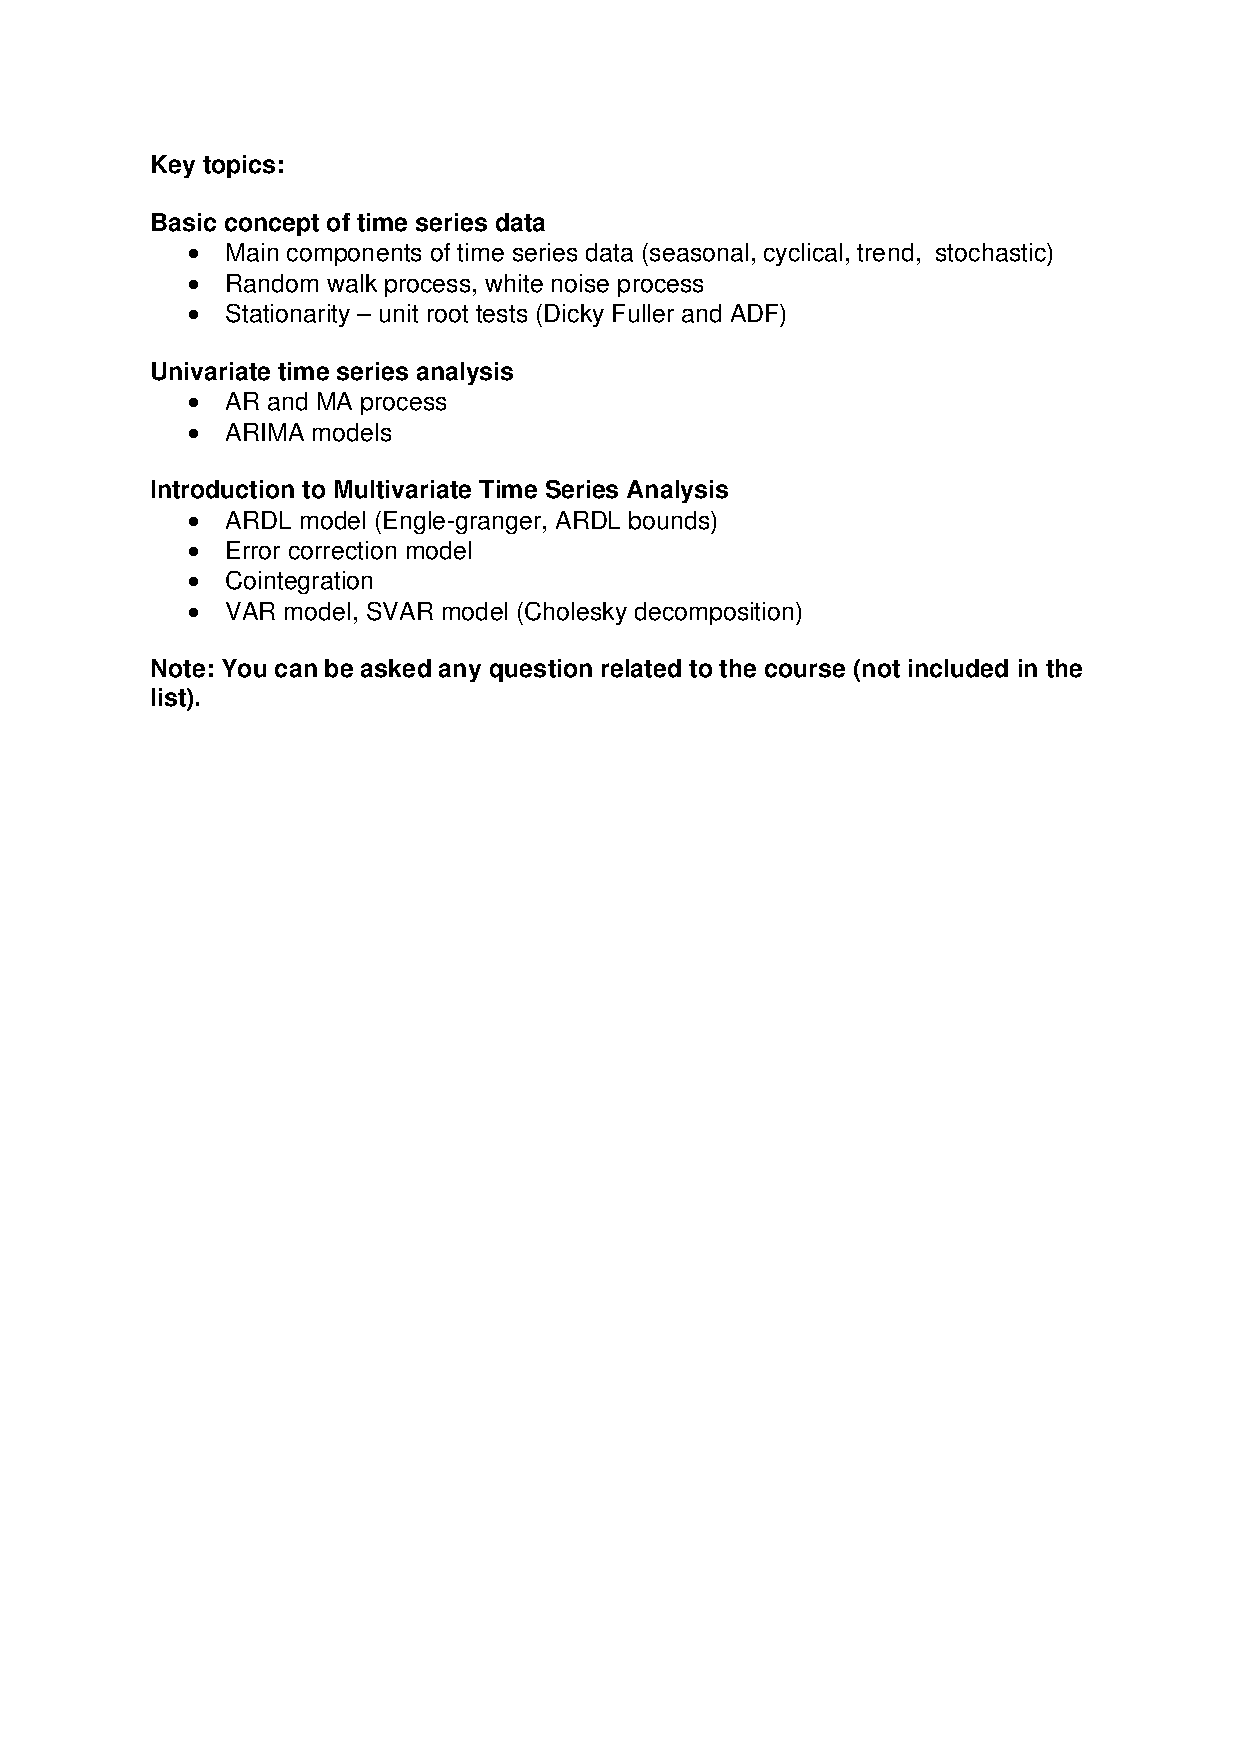
\includepdf[pages=1,pagecommand=\subsection{Teoretisk del}, offset=-1cm -3cm]{teory}

\hypertarget{basic-concepts-of-time-series-data}{%
\subsection{Basic concepts of time series
data}\label{basic-concepts-of-time-series-data}}

\hypertarget{main-components-of-time-series-dataseasonal-cyclical-trend-stocastic}{%
\subsubsection{\texorpdfstring{Main components of time series
data(seasonal, cyclical, trend, stocastic)\\
}{Main components of time series data(seasonal, cyclical, trend, stocastic) }}\label{main-components-of-time-series-dataseasonal-cyclical-trend-stocastic}}

En typisk tidsserie kunne opskrives på følgende måde:
\[X_t=seasonal_t+trend_t+cyclical_t+\epsilon_t \] Hvor vi har følgende
komponenter:\\
- Seasonal: Variablen kan være påvirket af forskellige sæsoner\\
- Cyclical: Variablen er påvirket af forskellige cyklusser (fx.
finansielle cykler)\\
- Trend: Variablen kan have en opadgående/nedadgående trend, eller ingen
trend\\
- Stocastic/Irregular variation: Den del, der gør tidsserien tilfældig,
fordi den har et randomt komponent.\\

\hypertarget{random-walk-process}{%
\subsubsection{Random walk process}\label{random-walk-process}}

En random walk process/model antager, at alle værdier tager et skridt
væk fra sin oprindelige værdi, når man lagger den med en periode. Der
findes en Random walk uden drift, der kan opskrives fra en AR(1) model,
hvor man sætter \(\theta=1\) og \(\mu=0\) \[ Y_t = Y_{t-1}+ \epsilon_t\]
Hvor fejlledet \(\epsilon_t\) følger en white-noise process:
\[\epsilon_t\sim IID(0,\sigma^2) \] Og hvor flere perioder
opskrives/udledes: \[Y_T=Y_{T-1}+\epsilon_T \]
\[Y_T=Y_{T-2}+\epsilon_{T-1}+\epsilon_T \] Hvor vi så kan lave et
generelt udtryk: \[Y_T=Y_0 + \sum_1^T \epsilon_t\] Nu skal vi huske
definitionen på stationære processor. Her husker vi, at mean(\(\mu\))
skal være uændret, når variansen er uændret. Det betyder altså, at de to
gerne skal være begrænsede konstanter. Så hvis vi udleder:
\[E\{Y_T\}=E\{Y_0+\sum_1^T\epsilon_t\}=Y_0 \tag{mean} \]
\[Var\{Y_T\}=Var\{Y_0+\sum_1^T\epsilon_t\}\]
\[Var\{Y_T\}=0+\sum_1^TVar\{\epsilon_t\}\]
\[Var\{Y_T\}=Var\{Y_0+\sum_1^T\epsilon_t\} \]
\[Var\{Y_T\}=T\sigma^2  \tag{Variance} \] Her kan vi se, at vores mean
er en konstant, mens vores varians er en funktion af tiden(T). Vi får
altså problemer med stationæritet i denne model. Dette kan dog løses ved
at tage differencen i vores tidsserie. Dette gør vi stor brug af i dette
kursus.\\
~\\
Udover Random walk uden drift, så kan vi også have random walk med
drift. Før tog vi afsæt i vores AR(1) model, hvor man satte \(\theta=1\)
og \(\mu=0\). Nu tillader vi at \(\mu\neq0\) og vi får dermed drift med
i modellen. Den opskrives nu indeholdende \(\mu\) da denne kan være
forskellig fra nul: \[ Y_t = \mu+ Y_{t-1}+ \epsilon_t\] Hvor fejlledet
\(\epsilon_t\) stadigvæk følger en white-noise process:
\[\epsilon_t\sim IID(0,\sigma^2) \] Afhængig af \(\mu\) vil tidsserien
nu drifte opad eller nedad. Dette kaldes også en stocastic
trend(tilfældig trend). Forskellen fra tidligere er, at nu er hverken
mean eller varians konstante. Dette kan vi udlede:
\[E\{Y_T\}=\mu+Y_{T-1}+\epsilon_T \]
\[= \mu+\mu+Y_{T-2}+\epsilon_{T-1}+\epsilon_T \]
\[=Y_0+\sum_1^T\mu+\sum_1^T\epsilon_T \]
\[E \{Y_0+\sum_1^T\mu+\sum_1^T\epsilon_T\} = Y_0+T\mu \tag{mean}  \] Her
kan vi se, at mean ikke er en konstant. Nu prøver vi med variansen:
\[ Var\{Y_T\}=Var\{Y_0+\sum_1^T\mu+\sum_1^T\epsilon_t\}      \]
\[ Var\{Y_T\} = 0+0+\sum_1^TVar\{\epsilon_t\} \]
\[ Var\{Y_T\} = T\sigma^2 \] Her kan vi også se, at variansen ikke er en
konstant. Vi har altså stadigvæk et problem med stationæritet, men dette
kan igen løses ved hjælp af at differenciere tidsserien \(Y_t\). Det
gøres således:\\
\[Y_t - Y_{t-1} = Y_{t-1} - Y_{t-1} + \epsilon_t \] På venstre side får
vi nu forskellen i \(Y_t\), og på venstre side går de to \(Y_{t-1}\) ud
med hinanden:\\
\[\underbrace{Y_t - Y_{t-1}}_\text{$\Delta Y_t$} = \underbrace{Y_{t-1} - Y_{t-1}}_\text{0} + \epsilon_t \]
Ved indsættelse får vi at:\\
\[\Delta Y_t = \epsilon_t \] Når en process kan laves stationær ved at
tage ``first difference'' så kaldes det får ``difference stationary
process''.\\

\hypertarget{white-noise-purely-random-process}{%
\subsubsection{White Noise (Purely Random
Process)}\label{white-noise-purely-random-process}}

Det er en stokastisk process som er en middelværdi på 0:
\[E(\epsilon_t) = 0\] En konstant varians: \[E(\epsilon_t^2)=\sigma^2\]
som ikke er seriekorreleret: \[E(\epsilon_t\epsilon_t)=0\]\\
for \(t\neq\tau\) Det kan skrives på måden\\
\[\epsilon_t \sim IID(0,\sigma^2)\]\\
Hvor IID står for en tilfældig variable der er individuelt og identisk
fordelt (independent and identically distributed).\\

\hypertarget{stationarity}{%
\subsubsection{Stationarity}\label{stationarity}}

Vi har to former for stationæritet:\\
Strict stationarity: som er en process, som forudsætter at ``joint
probability distribution'' af en tilfældig variabel ikke forandrer sig
over tid.\\

En joint probability funktion har forskellige moments/øjeblikke afhængig
af tidsperioden. En strict stationarity skal være uforanderlig over hele
perioden. Vi arbejder dog også med weak stationarity.\\

Weak stationarity: forudsætter, at det kun er de to første
moments/øjeblikke, der er uforanderlige. Det betyder altså, at mean(uden
trend) skal være uforandret, når variansen er uforandret. Disse to
``følger hinanden'' - Groft sagt.\\
I dette kursus arbejder vi mest med weak stationarity. Da det er det
mest sandsynlige i reel data.\\

\hypertarget{trend--versus-difference-stationary-series}{%
\subsubsection{Trend- Versus Difference-Stationary
Series}\label{trend--versus-difference-stationary-series}}

Når man taler om trends i tidsserier, så kan der være to forskellige
former for trends. Vi har en forudsigelig trend, som altid vender
tilbage til den langsigtede ligevægt ved stød. Hvis denne trend fjernes
fra dataet, får vi en tilfældig stationær process. Dette kaldes også for
en Trend-stationary serie.

Derudover så har vi en difference-stationary serie, hvor trenden kan
være tilfældig. Her vil stød være permanente, fordi man aldrig vil vende
tilbage til den langsigtede ligevægt. Her skal man differencere serien
med sig selv x-antal gange for at få en tilfældig stationær process.\\

\hypertarget{unit-root-testsdickey-fuller-and-adf}{%
\subsubsection{Unit root tests(Dickey Fuller and
ADF)}\label{unit-root-testsdickey-fuller-and-adf}}

Dickey-fuller testen bruges til at teste for unit roots i tidsserie.
ADF-testen er en advanceret version af denne. Vi udleder Dickey-fuller
testen nedenfor:\\
Vi starter med at opskrive en variable \(Y_t\) på en AR(1) process\\
\[Y_t = \theta Y_{t-1} + \epsilon_t\] Så trækkes \(Y_{t-1}\) fra på
begge sider \[ Y_{t} - Y_{t-1}=\theta Y_{t-1}-Y_{t-1}+\epsilon_{t} \] Vi
trækker den nutidige værdi fra den tidligere værdi for at få
\(\Delta Y_t\), og \(Y_t\) sættes uden for parantes
\[\Delta Y_t=(\theta-1)Y_{t-1}+\epsilon_t    \] Vi kalder \((\theta-1)\)
for \(\pi\) for at generalisere.
\[\Delta Y_t=\pi Y_{t-1} + \epsilon_t    \]

Hvor vi antager at \(\epsilon\) følger en white noise process.\\
\[\epsilon \sim IID(0,\sigma^2)\]\\
Der gælder forskellige ting for \(\theta\) :\\
Hvis \(|\theta|\) \(<\) 1 så er det en stationær process\\
Hvis \(|\theta|\) = 1 så er der unit root i tidsserien, og processen er
ikke stationær\\
Hvis \(|\theta|\) \(>\) 1 så eksplodere processen\\
~\\
Når vi laver en unit root test, så bruger vi\\
\textbf{Nulhypotesen}: \[H_0: \theta = 1 \tag{Unit root} \]
\textbf{Alternative hypotese}: \[H_1: \theta < 1 \tag{No unit root}\]

Grunden til vi tester om theta er mindre end 1 er, at det kun er der
hvor det er en stationær process. Vi kan altså ikke bruge den
alternative hypotese at theta er forskellige fra 1.\\
Efter omskriv så kan vi opskrive vores hypoteser på følgende måde\\
\textbf{Nulhypose}: \[H_0: \pi = 0 \tag{Unit root}\]
\textbf{Alternative hypotese} \[H_1: \pi < 0 \tag{No unit root}\]

Der gælder for Dickey-Fuller testen at hvis \(\pi = 0\) så er
\(\theta = 1\), og det betyder at der er unit root i vores tidsserie. Vi
skal ikke bruge vores almindelige t-værdier, men derimod sammenligne dem
med DF(tau)-statistikkerne som kan ses i appendix under tau-kritiske
værdier.

\newpage

\hypertarget{univariate-time-series-analysis}{%
\subsection{Univariate time series
analysis}\label{univariate-time-series-analysis}}

\hypertarget{auto-regressive-ar}{%
\subsubsection{Auto regressive (AR)}\label{auto-regressive-ar}}

En tidsserie er en AR hvis nutidige værdier af tidsserien kan blive
fundet ud fra tidligere værdier af tidsserien. Dette kan opskrives på
ligningen med ordnen p
\[y_t = c + \beta_1y_{t-1} + \beta_2y_{t-2} + \ldots + \beta_py_{t-p}+ \epsilon_t\]
Hvor c er en konstant(intercept), og hvor antallet af laggede værdier
kan bestemmes af ACF og PACF.\\
Hvis vi skal bruge en AR(1), så kan det opskrives som nedenfor
\[y_t = c + \beta_1y_{t-1} + \epsilon_t\] Eksempler kan være aktiepriser
og temperaturen.\\

\hypertarget{moving-average-ma}{%
\subsubsection{Moving average (MA)}\label{moving-average-ma}}

Det er en process hvor den nutidige værdi af en serie er bestemt af en
linær kombination af tidligere fejlled. Vi antager generelt set at
fejlledene er normalfordelt. Dette kan opskrives med ordnen q, ordnen
angiver hvor mange lags der skal med.
\[y_t = c + \epsilon_t + \beta_2\epsilon_{t-1} + \beta_3\epsilon_{t-2}+ \ldots + \beta_q\epsilon_{t-q}\]
Hvor \(\epsilon_t\) er en white noise process. Hvis vi vil se på en
MA(1) process, så ser den ud som nedenfor:
\[y_t = c + \epsilon_t + \beta_2\epsilon_{t-1}\] Vi har brugt andre
beta-værdier for at gøre det mere tydeligt at der er tale om to
forskellige processer.\\

\hypertarget{autoregressive-moving-average-models-arma}{%
\subsubsection{Autoregressive-moving-average models
(ARMA)}\label{autoregressive-moving-average-models-arma}}

ARMA modeller kan bruges til at fortolke eller forecaste på tidsserier.
Delen med AR der laver man en regression på variablens laggede værdier,
hvor MA delen er en regression af den linærer samling af fejlled. ARMA
modeller beskrives oftest som ARMA(p,q), hvor p angiver ordnen for AR
delen, og q angiver ordnen for MA delen.\\

\hypertarget{autoregressive-integrated-moving-average-arima}{%
\subsubsection{Autoregressive integrated moving average
(ARIMA)}\label{autoregressive-integrated-moving-average-arima}}

Det er en model der bygger ovenpå en ARMA model, og de kan begge bruges
til at forecaste tidsserier med.\\
En ARIMA(1,0,0) er en AR(1), en ARIMA(0,1,0) er en I(1) og en
ARIMA(0,0,1) er en MA(1) process.\\
\[ARIMA\underbrace{(p,d,q)}_\text{(den ikke stationærer del af modellen)}\underbrace{(P,D,Q)}_\text{(sæson delen af modellen)}\]

\newpage

\hypertarget{introduction-to-multivariate-time-series-analysis}{%
\subsection{Introduction to multivariate Time Series
Analysis}\label{introduction-to-multivariate-time-series-analysis}}

\hypertarget{cointegration}{%
\subsubsection{Cointegration}\label{cointegration}}

Cointegration opstår, når to eller flere variable har et langsigtet
forhold med hinanden. Ofte bliver det langsigtede forhold beskrevet som
en ligevægt, som modeller vender tilbage til ved stød eller lignende.
Man vil gerne have cointegration i sine modeller, da man så bedre kan
arbejde med dem uanset om det I(0) eller I(1\ldots.x)-processer. Det kan
man fordi, at de altid finder tilbage til den samme ligevægt, og det
derfor er optimalt at anvende dem til estimering og forecasting.

\hypertarget{error-correction-modelecm}{%
\subsubsection{Error correction
model(ECM)}\label{error-correction-modelecm}}

Når der er cointegration mellem flere variable, så vil der opstå
perioder, hvor variablerne differenciere sig fra hinanden i form af fx.
et stød eller andre faktorer, der gør, at de afviger fra den langsigtede
ligevægt. Ved cointegration vil de altid komme tilbage til den
langsigtede ligevægt, men det kan ikke siges, hvornår præcis dette sker.
Her kommer ECM-modellen i spil. Med modellen kan man estimerer
afvigelsen fra den langsigtede ligevægt. ECM-modellen kan altså bruges
til at finde ``speed of adjustment'' i vores variable.\\

Her skal vi huske, at hvis der ikke er cointegration, så er der risiko
for, at modellerne ikke konvergerer mod den langsigtede ligevægt, men
istedet kommer længere og længere væk fra hinanden.

\hypertarget{autoregressive-distributed-lag-modelardl}{%
\subsubsection{Autoregressive distributed lag
model(ARDL)}\label{autoregressive-distributed-lag-modelardl}}

En ARDL-model tager højde for de samme ting, som ECM-modellen, men den
er specificeret på en anden måde. Det langsigtede forhold er stort set
det samme som i ECM-modellen, og om man bruger den ene eller anden er
mere et spørgsmål om præference frem for reel funktion.

\hypertarget{engle-granger-procedure}{%
\subsubsection{Engle-Granger Procedure}\label{engle-granger-procedure}}

Engle-Granger kan bruges til at teste for cointegration. Dette kan gøres
på to eller flere variable. Hvis vi har at gøre med to variable, så er
der ikke cointegration, hvis begge variable er stationære, eller hvis de
er af forskellige order of integration. Hvis vi har med tre eller flere
variable at gøre, så gælder det at minimum to af disse, skal have samme
order of integration. Første step i Engle-Granger proceduren er altså at
finde order of integration ved hjælp af fx. en ADF-test. Dette uddyber
vi i ``Basic concepts of time series data''.\\

Når vi så har konkluderet, at der et langsigtet forhold(cointegration)
mellem vores variable, kan man opstille en ECM model. Her ville vi kunne
bruge OLS til parameter estimation og bla. få estimatoren speed of
adjustment, som er ret interessant i makroøkonomi.\\

En af problemerne/begrænsningerne ved ECM er, at den kører i flere
steps. Og hvis man laver fejl i step 1, så bliver den videreført i step
2, fordi man bruger residualerne fra step 1. Dette kunne fx. være
misspecifikation, som kom med videre i hele modellen, og man dermed fik
biased resultater.

\hypertarget{vector-autoregressive-var-modeller}{%
\subsubsection{Vector autoregressive (VAR)
modeller}\label{vector-autoregressive-var-modeller}}

VAR modeller bliver brugt til at forecaste fremtidige værdier af
variable, hvor der differentieres mellem VAR, RVAR og SVAR.

\textbf{Den simple form for VAR}\\
Vi vil i dette afsnit beskrive den simple form for VAR, og opskrive den
på matematisk form. En VAR model kan bruges til at beskrive
sammenhængene mellem flere variable både i nutidige og tidligere
perioder. Det er en meget anderkendt og brugt økonometrisk metode i dag.
Vi vil nu opskrive metoden på ligningsform, hvor vil bruge de tre
variable \(x\), \(y\) og \(z\).

\[x_t=b_{10}-b_{12}z_t-b_{13}y_t+a_{11}x_{t-1}+a_{12}z_{t-1}+a_{13}y_{t-1}+e_{1t} \]
\[z_t=b_{20}-b_{21}x_t-b_{23}y_t+a_{21}x_{t-1}+a_{22}z_{t-1}+a_{23}y_{t-1}+e_{2t} \]
\[y_t=b_{30}-b_{31}x_t-b_{32}z_t+a_{31}x_{t-1}+a_{32}z_{t-1}+a_{33}y_{t-1}+e_{3t} \]

Flytter alle termer med nutidige værdier over på venstresiden:

\[x_t+b_{12}z_t+b_{13}y_t=b_{10}+a_{11}x_{t-1}+a_{12}z_{t-1}+a_{13}y_{t-1}+e_{1t} \]
\[b_{21}x_t+z_t+b_{23}y_t=b_{20}+a_{21}x_{t-1}+a_{22}z_{t-1}+a_{23}y_{t-1}+e_{2t} \]
\[b_{31}x_t+b_{32}z_t+y_t+b_{30}+a_{31}x_{t-1}+a_{32}z_{t-1}+a_{33}y_{t-1}+e_{3t} \]

Opstiller på matrice form:

\[ \underbrace{
\left[ \begin{array}{ccc}
1 & b_{12} & b_{13} \\
b_{21}  & 1 & b_{23} \\
b_{31}  & b_{32} & b_{1}
\end{array} \right] }_{B} 
\underbrace{
\left[ \begin{array}{c}
x_{t} \\
z_{t} \\
y_{t} 
\end{array} \right] }_{y_t} 
=
\underbrace{
\left[ \begin{array}{c}
b_{10} \\
b_{20}  \\
b_{30}
\end{array} \right] }_{\Gamma_0}  +
\underbrace{
\left[ \begin{array}{ccc}
a_{11} & a_{12} & a_{13} \\
a_{21} & a_{22} & a_{23}\\
a_{31} & a_{32} & a_{33}
\end{array} \right] }_{\Gamma_1} 
\underbrace{
\left[ \begin{array}{c}
x_{t-1} \\
z_{t-1} \\
y_{t-1}
\end{array} \right] }_{y_{t-1}}  + 
\underbrace{
\left[ \begin{array}{c}
e_{1 t} \\
e_{2t} \\
e_{3t}
\end{array} \right] }_{e_t} \]

For at gøre det mere overskueligt kan det opstilles på en generel form,
hvor de forskellige værdier er angivet i underbrackets under deres
respektive matricer. \[ By_t=\Gamma_0+\Gamma_1y_{t-1}+e_t\]

Den generelle form er ikke påvirket af antallet af variable og vil
derfor altid forblive den samme.\\

Generelle VAR modeller kan ikke estimeres, da der er interaktion mellem
\(x_t\), \(y_t\) og \(z_t\). Dette har resulteret i et andet framework,
der kaldes en Reduced VAR model, som kan estimeres ved hjælp af OLS.
\newpage

\textbf{Reduced form VAR model (RVAR)}\\
Vi opskriver først VAR på den generelle form:
\[ By_t=\Gamma_0+\Gamma_1y_{t-1}+e_t\] Flytter matricen \(B\)
\[ y_t=B^-\Gamma_0+B^-\Gamma_1y_{t-1}+B^-e_t\]

Vi kan ikke estimere modellen hvor de nutidige værdier for \(x\) og
\(z\) optræder flere steder i de to ligninger, så vil effekterne af
deres samtidige effekter fanges i fejlleddet. Derfor angiver vi nu
parametrene som funktioner af VAR modellens parametre. Vi opstiller dem
derfor som A matricer og kalder \(\epsilon\) for fejlledet. Dette gøres
for at illustrere, at vi er gået fra en generel VAR model til en Reduced
form VAR model.
\[ y_t=\underbrace{B^-\Gamma_0}_{A_0}+\underbrace{B^-\Gamma_1}_{A_1}y_{t-1}+\underbrace{B^-e_t}_{\epsilon}\]
Så vi får: \[ y_t = A_0+A_1y_{t-1}+\epsilon\] Modellen kan nu estimeres,
da der ikke længere er missspecifikation i modellen/fejlledet.\\
Kritikken på RVAR modellen går på, at man går ind og fjerner nogle
komponenter for at kunne estimere. Det er derfor ikke den bedst mulige
estimation. I 1980 publicerer Christopher A. Sims en artikel, der skal
løse problemerne med at estimere uden restriktioner. Dette bliver kaldt
for Structural VAR modeller, og kan estimere mange variable på tværs af
tidsperioder uden restriktioner. Denne vil vi beskrive nedenfor.\\

\textbf{Structural VAR model (SVAR)}\\
I SVAR modellen tillader vi variable at påvirke hinanden på samme tid,
og det er derfor den type VAR model, hvor der er færrest restriktioner,
som rent faktisk kan estimeres. Forskellen fra VAR er, at her vil vi
ikke lade \(x\) blive påvirket i samme periode af \(z\) og \(y\). Vi vil
istedet lade \(z\) blive påvirket af \(x\) i samme periode, og \(y\) vil
vi lade blive påvirket af \(z\) og \(x\) i samme periode.\\
Modellen opstilles:

\[x_t=b_{10}+a_{11}x_{t-1}+a_{12}z_{t-1}+a_{13}y_{t-1}+e_{1t} \]
\[z_t=b_{20}-b_{21}x_t+a_{21}x_{t-1}+a_{22}z_{t-1}+a_{23}y_{t-1}+e_{2t} \]
\[y_t=b_{30}-b_{31}x_t-b_{32}z_t+a_{31}x_{t-1}+a_{32}z_{t-1}+a_{33}y_{t-1}+e_{3t} \]

Flytter nutidige værdier over på venstre side:
\[x_t=b_{10}+a_{11}x_{t-1}+a_{12}z_{t-1}+a_{13}y_{t-1}+e_{1t} \]
\[b_{21}x_t+z_t=b_{20}+a_{21}x_{t-1}+a_{22}z_{t-1}+a_{23}y_{t-1}+e_{2t} \]
\[b_{31}x_t+b_{32}z_t+y_t=b_{30}+a_{31}x_{t-1}+a_{32}z_{t-1}+a_{33}y_{t-1}+e_{3t} \]

Opskriver på matrice form: \[ \underbrace{
\left[ \begin{array}{ccc}
1 & 0 & 0 \\
b_{21}  & 1 & 0 \\
b_{31}  & b_{32} & 1
\end{array} \right]
}_{B}
\underbrace{
\left[ \begin{array}{c}
x_{t} \\
z_{t} \\
y_{t} 
\end{array} \right]
}_{y_t}
=
\underbrace{
\left[ \begin{array}{c}
b_{10} \\
b_{20}  \\
b_{30}
\end{array} \right]
}_{\Gamma_0}  
+
\underbrace{
\left[ \begin{array}{ccc}
a_{11} & a_{12} & a_{13} \\
a_{21} & a_{22} & a_{23}\\
a_{31} & a_{32} & a_{33}
\end{array} \right]
}_{\Gamma_1}
\underbrace{
\left[ \begin{array}{c}
x_{t-1} \\
z_{t-1} \\
y_{t-1}
\end{array} \right]
 }_{y_{t-1}}
 + 
\underbrace{
\left[ \begin{array}{c}
e_{1 t} \\
e_{2t} \\
e_{3t}
\end{array} \right]
 }_{e_t} \]

Vi har nu en model, der kan estimeres, som ikke undlader variable, og
hvor der er færest mulige restriktioner.

\hypertarget{cholesky-decomposition}{%
\subsubsection{Cholesky decomposition}\label{cholesky-decomposition}}

Cholesky decomposition er en metode i linæer algebra til at løse linæere
systemer, som siger:\\
Hvis \(A\) er en symmetrisk, positiv og afgrænset(definite) matrice, så
er der minimum en ``lower-triangle-matrix'' \(L\) som: \[ A=LL^T\]
Cholesky decomposition kan altså bruges til at lave en
``lower-triangle-matrix'', og bruges ofte til at udregne den inverse
matrice \(A^{-1}\) og determinanten af \(A\).

\newpage

\hypertarget{flere-begreber}{%
\subsection{Flere Begreber}\label{flere-begreber}}

\textbf{Unit root}:\\
Det er en stokastisk trend(kunne være random walk), som er et problem
når man arbejder med tidsseriemodeller.\\

\textbf{Cointegration}:\\
Hvis der findes en stationær linær sammenhæng mellem nogle variable, der
ikke er stationære, så siges det at variablerne er cointegrated. Et
eksempel på to variable der er cointegrated er en fuld person og
personens hund (Murray, 1994). Når den fulde er ude og gå med sin hund,
så løber hunden rundt omkring, og det ligner ikke der er en linær
sammenhæng. De er dog ude at gå en tur sammen, og de starter og slutter
det samme sted. Det skaber en linær sammenhæng.\\

\textbf{Philip-Perron test (PP test)}\\
Det er en statistisk test lavet af Peter C. B. Phillips og Pierre
Perron, som undersøger om der er unit root i en tidsserie.\\

\textbf{White Noise (Purely Random Process)}\\
Det er en stokastisk process som er en middelværdi på 0:
\[E(\epsilon_t) = 0\] En konstant varians: \[E(\epsilon_t^2)=\sigma^2\]
som ikke er seriekorreleret: \[E(\epsilon_t\epsilon_t)=0\]\\
for \(t\neq\tau\) Det kan skrives på måden\\
\[\epsilon_t \sim IID(0,\sigma^2)\]\\
Hvor IID står for en tilfældig variable der er individuelt og identisk
fordelt (independent and identically distributed).\\

\textbf{Zivot and Andrews testen (ZA testen)}:\\
Det er en test for strukturelle brud i en tidsserie, men ZA testen kan
kun finde et strukturelt brud, selvom det er meget muligt der er mere
end et strukturelt brud i tidsserien. Når man laver ZA testen, så er det
muligt at vælge mellem tre funktioner. Den første er ingen trend og
ingen trend. Den anden er intercept men ingen trend. Den sidste er at
både at have intercept og trend med.

\textbf{Seriekorrelation(autokorrelation)}:\\
Seriekorrelation kan beskrives som forholdet mellem en variabel og dens
laggede version af sig selv. Så man måler forholdet mellem variablens
nutidige værdi med en tidligere værdi. Seriekorrelation resulterer i
Biased resultater og bryder med TS5.

\textbf{Autocorrelation Function (ACF)}:\\
Det er en funktion der beskriver hvordan nutidige værdier af en serie
relatere sig til tidligere værdier af tidsserien. ACF kan på en gang
medtage trend, seasonality, cyclic og residualet når ACF undersøger for
korrelationer.\\

\textbf{Partiel Autocorrelation Function (PACF)}:\\
Det er en funktion der finder korrelationen af residualerne og den næste
laggede værdi, og den er partiel fordi vi fjerner tidligere fundet
variation inden vi finder den næste korrelation.\\

\textbf{Forecast bias}:\\
Det er når der er stor for forskel på de rigtige værdier af en variable,
og de værdier der blev blev forecastet. Det kan være at en model har det
med at forecaste for høje værdier af en variable.\\

\textbf{The lag operators}:\\
Til en konstant \begin{equation}
L(\alpha) = \alpha  \\
\end{equation} Til en variable \begin{equation}
L(x_t) = x_{t-1}  \\
\end{equation} Dobbelt lag til en variable \begin{equation}
L^2(x_t) = L[L(x_{t-1})]=L(x_{t-1})= x_{t-2} \\
\end{equation} Lag opløftede i n til en variable \begin{equation}
L^n(x_t) = x_{t-n}  \\
\end{equation} Den nutidige værdi af en variable hvor den laggede
trækkes fra \begin{equation}
(1-L)x_t = x_{t}-L(x_t)=x_t-x_{t-1}=\Delta x_t  \\
\end{equation} Forskellen mellem den laggede værdi af en periode, og den
laggede værdi af to perioder \begin{equation}
L(1-L)x_t = (1-L)x_{t-1}= x_{t-1} - L(x_{t-1}) = x_{t-1} + x_{t-2} =\Delta x_{t-1}\\
\end{equation}

\textbf{Fitted values (fittede værdier)}:\\
Alle tidsserier kan bruges til at lave forecast på baggrund af de
tidligere værdier af tidsserien. De fittede værdier er de forecastede
værdier af en variable, så hvis vores variable vi forecaster er \(y_t\),
så vil de fittede værdier være \(\hat{{y}}_{(t|t-1)}\).\\
Eksempel med BNP som værende tidsserien, så vil de fittede værdier være
\(\hat{{BNP}}_{(t|t-1)}\)\\

\textbf{Procylical variable}:\\
En variable der flukturer på en måde, som har en positiv korrelation med
BNP.

\textbf{Countercyclical variable}\\
En variable der flukturer på en måde, som har en negativ korrelation med
BNP.\\

\textbf{Sæsonjustere data}\\
Økonomisk data kan have sæsoneffekter i sig, det kunne være
husholdningers forbrug der generelt er større omkring jul end resten af
året. Når man sæsonjustere data, så forsøger man at fjerne
sæsoneffekterne. Grunden til man vil sæsonjustere data er for at gøre
det nemmere at sammenligne data.\\
Dette gøres ved at finde residualerne for ens variabel, og finde
gennemsnittet af ens fitted værdier og lægge de to sammen så:
\[ Residuals \ + mean(fitted.values)  \]

\textbf{F.test}\\
En F-test bruges til at sammenligne spredninger (kunne også være
varianser). Testen bliver lavet på samme måde som en t-test, men
test-størrelsen beregnes anderledes. Til F-test der bruges også en
F-fordeling til at beregne testsandsynligheden.\\

\textbf{Shapiro.test (Shapiro-Wilk test)}\\
Det er en test for normality, og undersøger om antagelse TS6 overholdes.
Der bruges p-værdier for at undersøge hypoteserne. Hypoteserne er givet
ved:

\[H_0:\ populationen \ er \ normalfordelt \]

\[H_1: \ populationen\ er\ ikke\ normalfordelt \]

\textbf{Jarque-Bera.test}\\
Det er en statistisk test der undersøger om dataet følger en
normalfordelingen, og testen undersøger derfor antagelse TS6.\\

\textbf{Engle.Granger test}\\
Det er en test for cointegration, som ser på om to variable har en
langsigtet effekt. Den bruger residualerne fra en regressionsmodel, og
så bruges en ADF test for at se om der unit root i residualerne. Hvis
der er unit root i residualerne så er variablene ikke cointegrated. Hvis
der ikke er unit root i residualerne, så er variablene cointegrated.
Testen kan kun bruges for variable som er af samme I process, men det må
ikke være over I(1).\\

\textbf{ARDL bounds test}\\
Det er en måde at undersøge om der er cointegration mellem variable, og
dermed også om der er langsigtede forhold mellem variablene. Denne
metode kan bruges selvom variablene både er i I(0) eller I(1) processer,
men den kan ikke bruges hvis variablene er i I(2) eller over.

\newpage

\textbf{Autoregressive distributed lag (ARDL) model}\\
Det er en model der bruges når man har med ECM at gøre. Det er en
regressionsmodel hvor koefficienterne ikke har restriktioner på samme
måde som de har med ECM.\\

\textbf{ECM}\\
Error correction modeller bliver brugt, når flere tidsserier har et
langsigtet forhold med hinanden. Dette kaldes også cointegration. Man
kan bruge dem til at estimere både kortsigtede og langsigtede effekter,
men også bruges til at estimere speed of adjustment.\\

\textbf{VECM}\\
Vector error correction model er en advanceret version af ECM, som kan
håndtere flere forskellige afhængige variable og forskellige langsigtede
forhold på tværs af hinanden. Denne model tager egentlig en VAR model og
tilføjer ECM til denne VAR model. Hvor man ville gøre følgende:\\
- Opstil en VAR model\\
- Teste for cointegration(langsigtede forhold)\\
- Anvende VECM til at analysere estimater\\

\textbf{Dickey-Fuller (DF) test }\\
Det er en test der kan bruges til at finde ud af om der er unit root i
ens data.\\

\textbf{Augmented Dickey-Fuller (ADF) test }\\
Den augmented Dickey-Fuller test bruges til at se om der er unit root i
ens data. Det der er anderledes ved ADF er, at en ADF test er bedre end
DF testen, og kan håndtere problemmet med seriekorrelation. Samtidig kan
en ADF test bruges til mere komplekse modeller end DF testen.\\

\textbf{Ljung-box test}\\
Det er en test for seriekorrelation (autokorrelation), og det betyder
den tester for fejlledet følger en white noise process. Hvis vi finder
at der er seriekorrelation, og fejlledet ikke følger en white noise
process, så er det fordi vi ikke har lavet en god regression. Det kan
være der mangler lags, vigtige variable osv.\\

\textbf{Auto-Regressive Conditional Heteroskedasticity (ARCH) test}\\
Det er en test der undersøger om antagelsen om homoskedasticitet holder.
Den har to test der gør mere eller mindre det samme: White's test og
Breusch-Pagan/Godfrey LM test.\\

\textbf{White's test}\\
Det er en test der bruges til at undersøge om variansen af ens fejlled
er konstant, altså om ens regression har heteroskedasitet i sig.\\

\textbf{Breusch-Pagan-Godfrey LM test}\\
Det er en test der bruges til at undersøge ens residualer for
heteroskedasitet.\\

\textbf{Residualer er normalfordelt}\\
Det er det samme som antagelse TS6, og det betyder at fejlledene følger
en normalfordeling og der ikke er væsentlige outliers.\\

\textbf{URCA pakken}\\
URCA pakken i \({\rm I\!R}\) har en læng række funktioner, som er
relevante i tidsserie økonometri. Vi gør mest brug af ADF testen(ur.df),
som tester for unit root, men vi har også anvendt bla. ur.za, som tester
for strukturelle brud.\\

\textbf{auto.arima pakken}\\
Auto arima pakken i \({\rm I\!R}\) retunerer den bedste ARIMA model med
hensyn til aicc, aic eller bic værdien.\\

\textbf{Out of sample forecast}\\
Out of sample forecasting er når man bruger alt ens data til at
forecaste fremtiden. Man bruger ofte den bedste model, som man har
fundet ved in-sample forecastingen.\\

\textbf{Spurious regressions}\\
Spurious betyder uægte/falsk og anvendes ofte om regressioner, forhold
eller lignende i statistikken. En falsk regression kan altså være en
regression, der viser et forkert forhold mellem to variable, fordi der
er unit root i dataet, og der ikke er taget højde for dette.\\

\textbf{Difference of variable}\\
Hvis vi har en variable \(Y_t\) som står for en tidsserie og Y indikere
at det er BNP. Så hvis vi skal tage ``first difference'' til \(Y_t\) så
kommer det til at se sådan her ud: \[\Delta Y_t = Y_t - Y_{t-1}  \] Hvis
vi nu skal tage ``difference'' til en variable vi allerede har taget
``first difference'' på (det kunne være \(\Delta Y_t\)) så kommer det
til at se sådan her ud: \[\Delta^2 Y_t =\Delta Y_t - \Delta Y_{t-1}  \]
Sådan kunne vi blive ved, og det er særlig relevant når vi snakker om at
skulle finde den rette I process.\\

\textbf{Glidende gennemsnit}\\
Det er en metode til at udglatte udsving i en variable ved brug af
tidligere værdier af variablen.\\

\textbf{Negativ $R^2$}\\
Det er ikke godt, og det betyder at de variable man har med i sin
regression ikke har særlig stor forklaringsgrad.\\

\hypertarget{udledninger}{%
\subsection{Udledninger}\label{udledninger}}

\hypertarget{basale-udledninger}{%
\subsubsection{Basale udledninger}\label{basale-udledninger}}

\textbf{Expected value}\\
Vi tager den forventede værdi til en konstant (a) ganget på en variable
(X), og så bliver konstanten (b) lagt til. Den forventede værdi til en
konstant er bare konstanten selv, så den kan man tage udenfor (a tages
udenfor):\\
\[E(aX+b) = aE(X) + b \] Den forventede værdi til en variable (X) lagt
til en anden variable (Y):\\
\[E(X + Y) = E(X) + E(Y) \] Den forventede værdi til to variable ganget
med hinanden. Der er det muligt at tage den forventede værdi af den ene
variable (E(X)) og gange den med den forventede værdi af den anden
variable (E(Y)). Det gælder kun hvis X og Y er uafhængige af hinanden:\\
\[E(XY) = E(X)E(Y) \]

\textbf{Variansen}\\
Variansen til en variable er givet på følgende måde:\\
\[Var(X) = E[X-E(X)]^2 = E(XX) - E(X)E(X) \] Når den forventede værdi af
variablen er lig nul (E(X)=0), så er variansen til variablen givet
ved:\\
\[Var(X) = E(X^2) \]\\
Variansen til en konstant (a) ganget på en variable (X), hvor der bliver
lagt en konstant til (b). Variansen til en konstant alene er 0
(Var(b)=0), og resten er givet ved:\\
\[Var(aX + b) = a^2Var(X) \] Variansen til to varable lagt sammen er
givet ved:\\
\[Var(X + Y) = Var(X) + Var(Y) + 2Cov(X,Y) \] Hvis X og Y er uafhængige,
så er variansen til to variable lagt sammen givet ved:\\
\[Var(X+Y) = Var(X) + Var(Y) \]

\newpage

\textbf{Covariance}\\
Kovariansen til to variable er givet ved:\\
\[Cov(X,Y) = E[X-E(X)][Y-E(Y)]=E(XY)-E(X)E(Y)\] Kovariansen til den den
samme variable er givet ved:\\
\[Cov(X,X) = Var(X) \] Kovariansen til en konstant (a) ganget med en
variable (X), hvor der bliver lagt en konstant til (b), med en anden
linær model (cY+d) på samme form:\\
\[Cov(aX+b,cY+d) = acCov(X,Y) \] Kovariansen til to variable lagt samme
overfor en anden variable er givet ved:\\
\[Cov(X+Y,Z) = Cov(X,Z) + Cov(Y,Z) \]

\newpage

\hypertarget{tidsserie-relevante-udledninger}{%
\subsubsection{Tidsserie-relevante
udledninger}\label{tidsserie-relevante-udledninger}}

\textbf{Partial autocorrelation function(PACF)}\\
Hvis vi har en AR(1) process:\\
\[Y_t = \theta_1 Y_{t-1} + \epsilon_t \] Som kan omskrives til en AR(2)
process ved at tilføje \(\theta_2 Y_{t-2}\):
\[Y_t = \theta_1 Y_{t-1} + \theta_2 Y_{t-2} + \epsilon_t \] Hvor
\(\theta_2\) er den partielle korrelation der er mellem \(Y_t\) og
\(Y_{t-2}\) mens alle effekter af \(Y_{t-1}\) holdes fast. Vi kan
opskrive dette på en mere genrel måde:\\
\[\theta_1 = \rho_1 \] Og
\[\theta_2 = \frac{\rho_2 - \rho_1^2}{1-\rho_1^2} \] De kan findes
direkte i \({\rm I\!R}\).\\

\textbf{General ARMA(p,q) Process}\\
Den generelle autoregressive moving average process (ARMA(p,q)) kan
opskrives som:\\
\[Y_t = \mu + \theta Y_{t-1} + \dots + \theta_p Y_{t-p} + \epsilon_t + \alpha_1 \epsilon_{t-1} + \dots + \alpha_q \epsilon_{t-q} \]
For at gøre det mere tydeligt hvilken del der er AR og hvilken del der
er MA, så har vi lavet følgende:\\
\[Y_t =\overbrace{\mu}^{\text{en konstant}} + \underbrace{\theta Y_{t-1} + \dots + \theta_p Y_{t-p}}_\text{AR del} + \overbrace{\epsilon_t}^{\text{et fejlled}} + \underbrace{\alpha_1 \epsilon_{t-1} + \dots + \alpha_q \epsilon_{t-q}}_\text{MA del} \]
Hvor at fejlledet følger en white noise process:\\
\[\epsilon_t \sim IID(0,\sigma^2) \] Hvis nu at vi har med ikke
stationært data, så skal vi lave en ARIMA(p,d,q) model.

\newpage

\textbf{Properties of forecasts}\\
Hvis vi starter med at antage en AR(1) process:\\
\[Y_t = \mu + \theta_1 Y_{t-1} + \epsilon_t \] Vi antager at fejlledet
følger en white noise process.\\
\[\epsilon_t \sim IID(0,\sigma^2) \] Hvis vi antager at vi kender
\(\mu\) og \(\theta_1\) så kan vi forcaste \(y_{t+1}\). Vi skal være
opmærksom på \(I_t\) altså hvilken order of integration serien er i
perioden t.\\
Vi kan udlede et ``one point ahead forecast'' betinget af vi kender
ordnen for integration. Når vi kigger på et forecast for næste periode
\(y_{t+1}\) så gøres det således:\\
\[E_t(y_{t+1})=E_t(\mu + \theta_1 y_t + \epsilon_t) \] Vi har antaget at
fejlledet havde en middelværdi på 0, så den bliver 0:\\
\[E_t(y_{t+1})=E_t(\mu) + E_t(\theta_1 y_t) + \underbrace{(\epsilon_t)}_\text{$0$} \]
Ved indsættelse fåes:\\
\[E_t(y_{t+1})=E_t(\mu) + E_t(\theta_1 y_t) + 0 \] Den forventede værdi
af en konstant (\(\mu\)) er konstanten selv.\\
\[E_t(y_{t+1})=\underbrace{E_t(\mu)}_\text{$\mu$} + E_t(\theta_1 y_t) \]
Ved indsættelse fåes:\\
\[E_t(y_{t+1})=\mu + E_t(\theta_1 y_t) \] Vi ved at
\(E_t(y_t|I_t)=y_t\), og derfor gælder at:\\
\[E_t(y_{t+1})=\mu + \underbrace{E_t(\theta_1 y_t)}_\text{$\theta_1 y_t$} \]
Ved indsættelse fåes:\\
\[E_t(y_{t+1})=\mu + \theta_1 y_t \] Dette var udledningen af et
forecast af en AR(1) process for en periode frem.\\
Det er også muligt at udlede et forecast for to perioder frem
\(y_{t+2}\), igen er det vigtigt at være opmærksom på at det er betinget
af \(I_t\). Det gør vi på følgende måde:\\
\[E_t(y_{t+2}) = E_t(\mu + \theta_1 y_{t+1} + \epsilon_{t+1})  \] Vi
antager at fejlledet følger en normal fordeling, og derfor er en
middelværdi på 0:\\
\[E_t(y_{t+2}) = E_t(\mu) + E_t(\theta_1 y_{t+1}) + E_t(\underbrace{\epsilon_{t+1} }_\text{$0$}) \]
Ved at sætte det ind får vi at:\\
\[E_t(y_{t+2}) = E_t(\mu) +E(\theta_1 y_{t+1}) + 0 \] Den forventede
værdi af en konstant (\(\mu\)) er bare konstanten:\\
\[E_t(y_{t+2}) = \underbrace{E_t(\mu)}_\text{$\mu$} + E(\theta_1 y_{t+1}) \]
Vi kan tage konstanten udenfor (\(\theta\)):\\
\[E_t(y_{t+2}) = \mu + \theta_1E(y_{t+1}) \] Vi indsætter
\(E(y_{t+1}) = \mu + \theta y_t\):\\
\[E_t(y_{t+2}) = \mu + \theta_1E\underbrace{(y_{t+1})}_\text{$\mu + \theta_1 y_t$} \]
Ved indsættelse fåes:\\
\[E_t(y_{t+2}) = \mu + \theta_1(\mu + \theta_1 y_t) \] Vi ganger nu ind
i parantesen: \[E_t(y_{t+2}) = \mu + \theta_1\mu + \theta_1^2 y_t \]
Dermed har vi fundet forecast for to perioder frem.\\
Vi kan opskrive et generelt forecast for \(y_{t+j+1}\):\\
\[E(y_{t+j+1})=E(y_{t+j+1}|I_t) \]

\newpage

\hypertarget{moving-average-process}{%
\subsubsection{Moving Average Process}\label{moving-average-process}}

Vi har en MA(1) process:\\
\[Y_t = \mu + \epsilon_t + \alpha \epsilon_{t-1} \] Vi antager at vores
fejlled \(\epsilon_t\) føger en normalfordeling.\\

\textbf{Calculate the mean of $Y_t$}\\
Det første vi skal gøre er at udregne den forventede værdi af \(Y_t\)\\
\[E(Y_t) = E\underbrace{(\mu + \epsilon_t + \alpha \epsilon_{t-1})}_\text{$Y_t$} \]
Vi starter med at gange E ind i parantesen, og tage den forventede værdi
til hvert led:\\
\[E(Y_t) = E(\mu) + E(\epsilon_{t-1}) + E(\alpha \epsilon_{t-1}) \]

Den forventede værdi til en konstant (\(\mu\)) er lig konstanten selv.
Da vi antog vores fejlled har en middelværdi på 0, så giver de begge
nul:
\[E(Y_t) = \underbrace{E(\mu)}_\text{$\mu$} + \underbrace{E(\epsilon_{t-1})}_\text{0} + \underbrace{E(\alpha \epsilon_{t-1})}_\textsc{0} \]
Det giver os at den forventede værdi til variablen (\(Y_t\)) er lig
\(\mu\):\\
\[E(Y_t) = \mu  \]

\textbf{Calculate the variance of $Y_t$}\\
Vi lader \(Y_t\) være givet ved:\\
\[Y_t = \mu + \epsilon_t + \alpha \epsilon_{t-1}\] Vi vælger nu at rykke
\(\mu\) over på venstre side:\\
\[Y_t - \mu = \epsilon_t + \alpha \epsilon_{t-1} \] Nu tager vi så
variansen af det: \[Var(Y_t) = E[(Y_t - \mu)^2] \] Vi ved at
\(Y_t - \mu\) er lig \(\epsilon_t + \alpha \epsilon_{t-1}\), så det
sætter vi ind:\\
\[Var(Y_t) = E[(\underbrace{(\epsilon_t + \alpha \epsilon_{t-1})}_\text{$Y_t - \mu $})^2] \]
Vi vælger nu at opløfte parantesen i forhold til at have det i anden
(\^{}2):\\
\[Var(Y_t) = E(\epsilon_t^2+2\alpha \epsilon_t \epsilon_{t-1} + \alpha^2 \epsilon_{t-1}^2) \]
Nu tager vi den forventede værdi til de tre led i ligningen:\\
\[Var(Y_t) = E(\epsilon_t^2) +2\alpha E(\epsilon_t \epsilon_{t-1}) + \alpha^2 E( \epsilon_{t-1}^2) \]
Vi har tidligere antaget at fejlledet har en middelværdi på 0, og det
betyder at \(E(\epsilon_t \epsilon_{t-1})=0\):\\
\[Var(Y_t) = E(\epsilon_t^2) + \underbrace{2\alpha E(\epsilon_t \epsilon_{t-1})}_\text{0} + \alpha^2 E( \epsilon_{t-1}^2) \]
Det giver os følgende:\\
\[Var(Y_t) = E(\epsilon_t^2) + \alpha^2E( \epsilon_{t-1}^2) \] Vi har
antaget at fejlledet havde en konstant varians \(\sigma^2\), og vi får
derfor følgende:\\
\[Var(Y_t) = \underbrace{E(\epsilon_t^2)}_\text{$\sigma^2$} + \alpha^2\underbrace{E(\epsilon_{t-1}^2)}_\text{$\sigma^2$} \]
Vi kan nu indsætte \(\sigma^2\) og få:\\
\[Var(Y_t) = \sigma^2 + \alpha^2\sigma^2 \] Vi kan nu tage \(\sigma^2\)
udenfor parantes:\\
\[Var(Y_t) = (1 + \alpha^2)\sigma^2 \] Vi har nu funder variansen for
\(Y_t\).\\

\textbf{Calculate the autocovariance between $Y_t$ and $Y_{t-1}$}\\
Vi starter med at lade \(Y_t\) være givet ved:\\
\[Y_t = \mu + \epsilon_t + \alpha \epsilon_{t-1} \] Vi vælger nu at
rykke \(\mu\) over på venstre side:\\
\[Y_t - \mu = \epsilon_t + \alpha \epsilon_{t-1} \] Vi lader \(Y_{t-1}\)
være givet ved\\
\[Y_{t-1} = \mu + \epsilon_{t-1} + \alpha \epsilon_{t-2} \] Vi vælger nu
at rykke \(\mu\) over på venstre side:\\
\[Y_{t-1} - \mu = \epsilon_{t-1} + \alpha \epsilon_{t-2} \] Vi vil nu
finde kovariansen mellem \(Y_t\) og \(Y_{t-1}\):\\
\[Cov(Y_t,Y_{t-1}) = E[(Y_t-\mu)(Y_{t-1}-\mu)] \] Vi indsætter nu
udtrykket \(Y_t - \mu = (\epsilon_t + \alpha \epsilon_{t-1})\)\\
\[Cov(Y_t,Y_{t-1}) = E[\underbrace{(\epsilon_t + \alpha \epsilon_{t-1})}_\text{$Y_t - \mu$}(Y_{t-1}-\mu)] \]
Nu sætter vi udtrykket
\(Y_{t-1} - \mu = (\epsilon_{t-1} + \alpha \epsilon_{t-2}\)) ind:\\
\[Cov(Y_t,Y_{t-1}) = E[\underbrace{(\epsilon_t + \alpha \epsilon_{t-1})}_\text{$Y_t - \mu$}\underbrace{(\epsilon_{t-1} + \alpha \epsilon_{t-2})}_\text{$Y_{t-1} - \mu$}] \]
Vi kan nu tage konstanten (\(\alpha\)) udenfor parantesen:\\
\[Cov(Y_t,Y_{t-1}) = \alpha E[(\epsilon_t + \epsilon_{t-1})(\epsilon_{t-1} + \epsilon_{t-2})] \]
Vi har to paranteser, og ved at gange dem sammen får vi
\(\epsilon_{t-1}^2\)\\
\[Cov(Y_t,Y_{t-1}) = \alpha E[\underbrace{(\epsilon_t + \epsilon_{t-1})(\epsilon_{t-1} + \epsilon_{t-2})}_\text{$\epsilon_{t-1}^2$}] \]
Vi får nu følgende:\\
\[Cov(Y_t,Y_{t-1}) = \alpha E(\epsilon_{t-1}^2) \]\\
Vi antog tidligere at fejlledet havde en konstant varians \(\sigma^2\),
og derfor får vi følgende:\\
\[Cov(Y_t,Y_{t-1}) = \alpha \underbrace{E(\epsilon_{t-1}^2)}_\text{$\sigma^2$}\]
Ved indsættelse fåes:\\
\[Cov(Y_t,Y_{t-1}) = \alpha \sigma^2\] Vi har nu fundet autocovariance
for \(Y_t\) og \(Y_{t-1}\).\\

\newpage

\textbf{Calculate the autocovariance between $Y_t$ and $Y_{t-2}$}\\
Vi starter med at lade \(Y_t\) være givet ved:\\
\[Y_t = \mu + \epsilon_t + \alpha \epsilon_{t-1} \] Vi vælger nu at
rykke \(\mu\) over på venstre side:\\
\[Y_t - \mu = \epsilon_t + \alpha \epsilon_{t-1} \] Vi lader \(Y_{t-2}\)
være givet ved\\
\[Y_{t-2} = \mu + \epsilon_{t-2} + \alpha \epsilon_{t-3} \] Vi vælger nu
at rykke \(\mu\) over på venstre side:\\
\[Y_{t-2} - \mu = \epsilon_{t-2} + \alpha \epsilon_{t-3} \] Vi vil nu
finde kovariansen mellem \(Y_t\) og \(Y_{t-2}\):\\
Vi indsætter nu udtrykket
\(Y_t - \mu = (\epsilon_t + \alpha \epsilon_{t-1})\)\\
\[Cov(Y_t,Y_{t-1}) = E[\underbrace{(\epsilon_t + \alpha \epsilon_{t-1})}_\text{$Y_t - \mu$}(Y_{t-1}-\mu)] \]
Nu sætter vi udtrykket
\(Y_{t-2} - \mu = (\epsilon_{t-2} + \alpha \epsilon_{t-3}\)) ind:\\
\[Cov(Y_t,Y_{t-1}) = E[\underbrace{(\epsilon_t + \alpha \epsilon_{t-1})}_\text{$Y_t - \mu$}\underbrace{(\epsilon_{t-2} + \alpha \epsilon_{t-3})}_\text{$Y_{t-2} - \mu$}] \]
Vi har nu to paranteser, hvor at når vi ganger dem sammen, så får vi
0:\\
\[Cov(Y_t,Y_{t-1}) = E[\underbrace{(\epsilon_t + \alpha \epsilon_{t-1})(\epsilon_{t-2} + \alpha \epsilon_{t-3})}_\text{0}] \]
Dermed får vi at:\\
\[Cov(Y_t,Y_{t-1}) = 0 \] Der gælder helt generelt at:\\
\[Cov(Y_t,Y_{t-k})=0 \] for alle \(k = 2,3,4, ... , k\).\\

\newpage

\textbf{Inverting an MA(1) process into AR($\infty$)}\\
Det første vi gør at opskrive en MA(1) process, bemærk vi skriver - og
ikke + fordi Hamid har det med i sine slids på denne måde. Normalt ville
man skrive + : \[Y_t = \epsilon_t  - \alpha \epsilon_{t-1} \] Vi ved fra
lag operators i appendix, at \(\epsilon_{t-1} = L(\epsilon_t)\) :
\[Y_t = \epsilon_t  - \underbrace{\alpha \epsilon_{t-1}}_\text{$\alpha L( \epsilon_t$)} \]
Ved indsættelse fåes: \[Y_t = \epsilon_t  - \alpha L(\epsilon_t) \] Da
vi har \(\epsilon_t\) til at optræde i begge led på højresiden, så kan
vi sætte udenfor parantes: \[Y_t = \epsilon_t(1 - \alpha L) \] Nu kan vi
rykke \((1 - \alpha L)\) over på venstresiden:
\[\frac{Y_t}{(1 - \alpha L)} = \epsilon_t \] Vi bruger det geometriske
theorem: \[\sum_{n=0}^\infty = ar^0 + ar^1 + ar^2 + \dots + ar^n \] Det
konvergerer mod \[\frac{a}{1-r} \] hvis at \(|r| < 1\) er opfyldt. Hvis
vi nu skal omskrive det til ovenstående, så skal vi antage at
\(r = \alpha L\):
\[\epsilon_t = (\alpha L)^0Y_t + (\alpha L)^1Y_t + (\alpha L)^2 Y_t + \dots + (\alpha L)^nY_t \]
Hvis vi gør brug af lag operator 2 og 4 fra appendix, så får vi at:
\[\epsilon_t = Y_t + \alpha^1 Y_{t-1} + \alpha^2 Y_{t-2} + \dots + \alpha^n Y_{t-n} \]
Det opskriver vi så det står på \(AR(\infty)\) form ved at tage alt
andet end \(Y_t\) på højresiden og flytte over på venstre siden:
\[\epsilon_t = Y_t + \underbrace{\alpha^1 Y_{t-1} + \alpha^2 Y_{t-2} + \dots + \alpha^n Y_{t-n}}_\text{Flyttes over på den anden side} \]
Vi får dermed \(Y_t\) til at stå alene, for at stille det på den pæneste
visuelle måde så står \(Y_t\) til venstre:
\[\epsilon_t Y_t = \epsilon_t - \alpha^1 Y_{t-1} - \alpha^2 Y_{t-2} - \dots - \alpha^n Y_{t-n} \]
Nu har vi omskrevet en MA(1) process til en AR(\(\infty\)).\\

\textbf{The ACF of an MA(1) process}\\
\[\rho_k = \frac{\overbrace{Cov(Y_t,Y_{t-k})}^{\alpha \sigma^2}}{\underbrace{Var(Y_t)}_\text{($(1+\alpha^2)\sigma^2$)}} \]
Ved indsættelse fåes:\\
\[\rho_k = \frac{\alpha \sigma^2}{(1+\alpha^2)\sigma^2} \] Vi har
\(\sigma^2\) både i tælleren og i nævneren, og kan derfor fjerne dem:\\
\[\rho_k = \frac{\alpha \xout{\sigma^2}}{(1+\alpha^2)\xout{\sigma^2}} \]
Det giver os:\\
\[\rho_k = \frac{\alpha}{(1+\alpha^2)} \] Hvis at \(k>1\) så gælder
at:\\
\[\rho_k = 0 \] Dette var udledningen af ACF for en MA(1) process.\\

\newpage

\hypertarget{autoregressive-processes}{%
\subsubsection{Autoregressive
Processes}\label{autoregressive-processes}}

Vi starter med at opskrive en AR(1) process:\\
\[Y_t = \mu + \theta Y_{t-1} + \epsilon_t \] Vi antager at fejlledet
følger en white noise process:\\
\[\epsilon_t \sim IID(0,\sigma^2) \]
\textbf{Calculate the mean of $Y_t$}\\
\[E(Y_t) = E(\mu + \theta Y_{t-1} + \epsilon_t) \] Vi tager nu den
forventede værdi til hvert led i parantesen. Den forventede værdi af en
konstant (\(\mu\)) er konstanten selv, så der skriver vi bare \(\mu\):\\
\[E(Y_t) = \mu + E(\theta Y_{t-1}) + E(\epsilon_t) \] Vi kan nu tage
konstanten ud af parantesen (\(\theta\)):\\
\[E(Y_t) = \mu + \theta E(Y_{t-1}) + E(\epsilon_t) \] Vi lader
\(Y_{t-1}\) være givet ved:\\
\[(Y_{t-1}) = \mu + \theta Y_{t-2} + \epsilon_{t-1} \] Vi sætter nu
udtrykket for \(Y_{t-1}\) ind:\\
\[(Y_t{}) = \mu + \theta E(\underbrace{\mu + \theta Y_{t-2} + \epsilon_{t-1}}_\text{$(Y_{t-1})$}) + E(\epsilon_t) \]
Da vi har antaget at fejlledet har en middelværdi på 0, så kan vi sætte
denne til 0:\\
\[E(Y_t) = \mu + \theta E(\mu + \theta Y_{t-2} + \epsilon_{t-1}) + \underbrace{E(\epsilon_t)}_\text{0} \]
Dermed får vi:\\
\[E(Y_t) = \mu + \theta E(\mu + \theta Y_{t-2} + \epsilon_{t-1}) \] Vi
ganger nu \(\theta E\) på alle led i parantesen:\\
\[E(Y_t) = \mu + \theta \mu + \theta^2 E(Y_{t-2}) + \theta E(\epsilon_{t-1}) \]
Vi lader nu \(Y_{t-2}\) være givet ved:\\
\[Y_{t-2} = \mu + \theta Y_{t-3} + \epsilon_{t-2} \] Vi indsætter nu
udtrykket for \(Y_{t-2}\):\\
\[E(Y_t) = \mu + \theta \mu + \theta^2 E(\underbrace{\mu + \theta Y_{t-3} + \epsilon_{t-2}}_\text{$(Y_{t-2})$}) + \theta E(\epsilon_{t-1}) \]
Vi ved at \(\theta E(\epsilon_{t-1})\) giver 0, så det opskriver vi
nu:\\
\[E(Y_t) = \mu + \theta \mu + \theta^2 E(\underbrace{\mu + \theta Y_{t-3} + \epsilon_{t-2}}_\text{$(Y_{t-2})$}) + \underbrace{\theta E(\epsilon_{t-1})}_\text{0} \]
Begge dele bliver sat ind og vi får:\\
\[E(Y_t) = \mu + \theta \mu + \theta^2 E(\mu + \theta Y_{t-3} + \epsilon_{t-2}) \]
Da \(\mu\) indgår i alle led, så kan vi sætte det udenfor parantes:\\
\[E(Y_t) = \mu (1 + \theta + \theta^2 + ... + \theta^\infty) \] Hvis at
\(|\theta|<1\) gælder, så får vi at:\\
\[E(Y_t) =\frac{\mu}{1-\theta} \] Nu har vi udregnet middelværdien for
\(Y_t\) for en Autoregressive process.\\

\textbf{Calculate the variance of $Y_t$}\\
Vi lader først \(Y_t\) være givet ved:
\[Y_t = \mu + \theta Y_{t-1} + \epsilon_t \] Hvis vi flytter \(\mu\)
over på venstreside får vi:\\
\[Y_t - \mu = \theta Y_{t-1} + \epsilon_t \] Vi lader nu \(y_t\) være
givet ved \(Y_t - \mu\):\\
\[\underbrace{Y_t - \mu}_\text{$y_t$} = \theta Y_{t-1} + \epsilon_t \]
Ved indsættelse fåes:\\
\[y_t = \theta Y_{t-1} + \epsilon_t \] Det som vi vil i denne udledning
er at finde variansen til \(Y_t\) med vi gør det på \(y_t\), husk at der
er forskel:\\
\[Var(y_t) = E[(y_t - E(y_t)^2] \] Vi får nu at:\\
\[Var(y_t) = E[(\theta y_{t-1} + \epsilon_t)^2] \] Vi tager nu den
forventede værdi til hvert led i parantesen, og vi ganger også (\(^2\))
ind i parantesen:\\
\[Var(y_t) = \theta^2 E(y_{t-1}^2) + E(\epsilon_t)^2 \] Vi ved at
variansen til fejlledet er konstant, og givet ved \(\sigma^2\):\\
\[Var(y_t) = \theta^2 E(y_{t-1}^2) + \underbrace{E(\epsilon_t)^2}_\text{$\sigma^2$} \]
Ved indsættelse fåes at:\\
\[Var(y_t) = \theta^2 E(y_{t-1}^2) + \sigma^2 \] Nu lader vi
\(y_{t-1}^2\) være givet ved \((\theta y_{t-2} + \epsilon_{t-1})^2\).
Ved at sætte dette ind får vi at:\\
\[Var(y_t) = \theta^2 E\underbrace{(y_{t-1}^2)}_\text{$(\theta y_{t-2} + \epsilon_{t-1})^2$} + \sigma^2\]
Ved indsættelse fåes:\\
\[Var(y_t) = \theta^2 E(\theta y_{t-2} + \epsilon_{t-1})^2 + \sigma^2\]
Dette kan vi blive ved med at gøre, for nu har \(y_{t-2}\), som der også
kan findes et udtryk for og sættes ind. Det gør vi dog ikke, men tager
derimod variansen \(\sigma^2\) udenfor parantes for at finde et generelt
udtryk:\\
\[Var(y_t) = \sigma^2 (1 + \theta^2 + \theta^4 + ... + \theta^\infty)\]
Hvis \(|\theta|<1\) gælder, så vi at:\\
\[Var(y_t) = \frac{\sigma^2}{1-\theta^2} \] Vi har nu fundet variansen
for \(Y_t\) for en autoregressive process.\\

\textbf{Calculate the variance of $Y_t$ - simpel metode}\\
Vi lader variansen af \(Y_t\) være givet ved:\\
\[Var(Y_t) = Var(\mu \theta Y_{t-1} + \epsilon_t) \] Vi tager nu
variansen til hvert led i parantesen:\\
\[Var(Y_t) = Var(\mu) + \theta^2 var(Y_{t-1}) + Var(\epsilon_t) \] Vi
antager at variansen til \(\mu\) at være 0, og at variansen til
fejlledet til at være konstant \(\sigma^2\):\\
\[Var(Y_t) = \underbrace{Var(\mu)}_\text{0} + \theta^2 var(Y_{t-1}) + \underbrace{Var(\epsilon_t)}_\text{$\sigma^2$} \]
Når vi sætter ind får vi at:\\
\[Var(Y_t) = 0 + \theta^2 var(Y_{t-1}) + \sigma^2 \] Nu vælger vi at
flytte \(\theta^2 var(Y_{t-1})\) over på venstre side:\\
\[Var(Y_t) - \theta^2 var(Y_{t-1}) =   \sigma^2 \] Hvis vi har at
\(|\theta|<1\) så har vi en stationær autoregressive provess, og det gør
vi kan sætte \(Var(Y_t)\) udenfor parantes. Bemærk at vi tidligere havde
\(var(Y_{t-1})\), men med vores antagelse om \(|\theta|<1\), så får vi
\(Var(Y_t)\):\\
\[Var(Y_t)(1-\theta^2)  =   \sigma^2 \] Vi kan nu få \(Y_t\) til at stå
alene på venstre side ved at flytte \((1-\theta^2)\) over på højre
side:\\
\[Var(Y_t)  = \frac{\sigma^2}{(1-\theta^2)}   \]

\textbf{Calculate the autocovariance between $Y_t$ and $(Y_{t-1})$}:\\
Vi starter med at opskrive ligningen som:\\
\[Cov(Y_t,Y_{t-1}) = E[(Y_t - \mu)(Y_{t-1} -\mu)]   \] Hvis at
\(|\theta| < 1\) gælder, så kan det omskrives til:\\
\[Cov(Y_t,Y_{t-1}) = \theta \frac{\sigma^2}{1-\theta^2}   \] Generelt
kan det skrives på formlen, hvis følgende gælder \(|\theta| < 1\),
dermed får vi at:\\
\[Cov(Y_t,Y_{t-1}) = \theta^{|s-t|} \frac{\sigma^2}{1-\theta^2}   \]
Hvor s og t er antallet af lags.\\

\textbf{Converting an AR(1) process into MA(\infty)}\\
Vi starter med at have en AR(1) process:\\
\[Y_t = \alpha Y_{t-1} + \epsilon_t \] Vi kan også skrive \(Y_{t-1}\)
som \(L(Y_t)\):\\
\[Y_t = \alpha \underbrace{Y_{t-1}}_\text{$L(Y_t)$} +\epsilon_t \] Ved
indsættelse fåes:\\
\[Y_t = \alpha L(Y_t) +\epsilon_t \] Nu kan vi flytte \(\alpha L(Y_t)\)
over på venstre side:\\
\[Y_t - \alpha L(Y_t) =  \epsilon_t \] Vi har nu to \(Y_t\) udtryk på
venstre side, og kan derfor sætte det udenfor parantes:\\
\[Y_t(1-\alpha) =  \epsilon_t \] Vi kan nu flytte \((1-\alpha)\) over på
højre side:\\
\[Y_t = \frac{\epsilon_t}{(1-\alpha)}  \] For en AR(1) process er det
afgørende at \(|\alpha|<1\) for at det er en stationær process.\\
Vi brugte det geometriske serie theorem for at finde frem til dette. Det
ser sådan her ud:\\
\[\sum_{n=0}^\infty =  ar^0 + ar^1 + ar^2 + ... + ar^n \] Det konvergere
mod:\\
\[\sum_{n=0}^\infty = \frac{\alpha}{1-r}  \] Så længe at \(|r|<1\).\\

\textbf{The ACF of an AR(1) process}\\
Vi starter med at antage weak stationarity, og definere ordnen for
autocovariancen som værende:\\
\[\gamma_k = Cov(Y_t,Y_{t+k})=Cov(Y_t,Y_{t-k}) \] Hvis at vi har med en
stokastisk process at gøre, så kan det generaliseres til:\\
\[\rho_k = \frac{Cov(Y_t,Y_{t-k})}{Var(Y_t)} \] Vi kender både udtrykket
for \(Cov(Y_t,Y_{t-k})\), og for \(Var(Y_t)\):\\
\[\rho_k = \frac{\overbrace{Cov(Y_t,Y_{t-k})}^{\theta^k (\sigma^2/1-\theta^2)}}{\underbrace{Var(Y_t)}_\text{($\sigma^2/1-\theta^2$)}} \]
Nu sætter vi ind i ligningen:\\
\[\rho_k = \frac{\theta^k ((\sigma^2/1-\theta^2))}{\sigma^2/1-\theta^2)} \]
Da vi har \((\sigma^2/1-\theta^2)\) både i tælleren og nævneren, så de
går ud med hinanden:\\
\[\rho_k = \frac{\theta^k \xout{(\sigma^2/1-\theta^2)}}{\xout{\sigma^2/1-\theta^2)}} \]
Dermed får vi:\\
\[\rho_k = \theta^k  \]

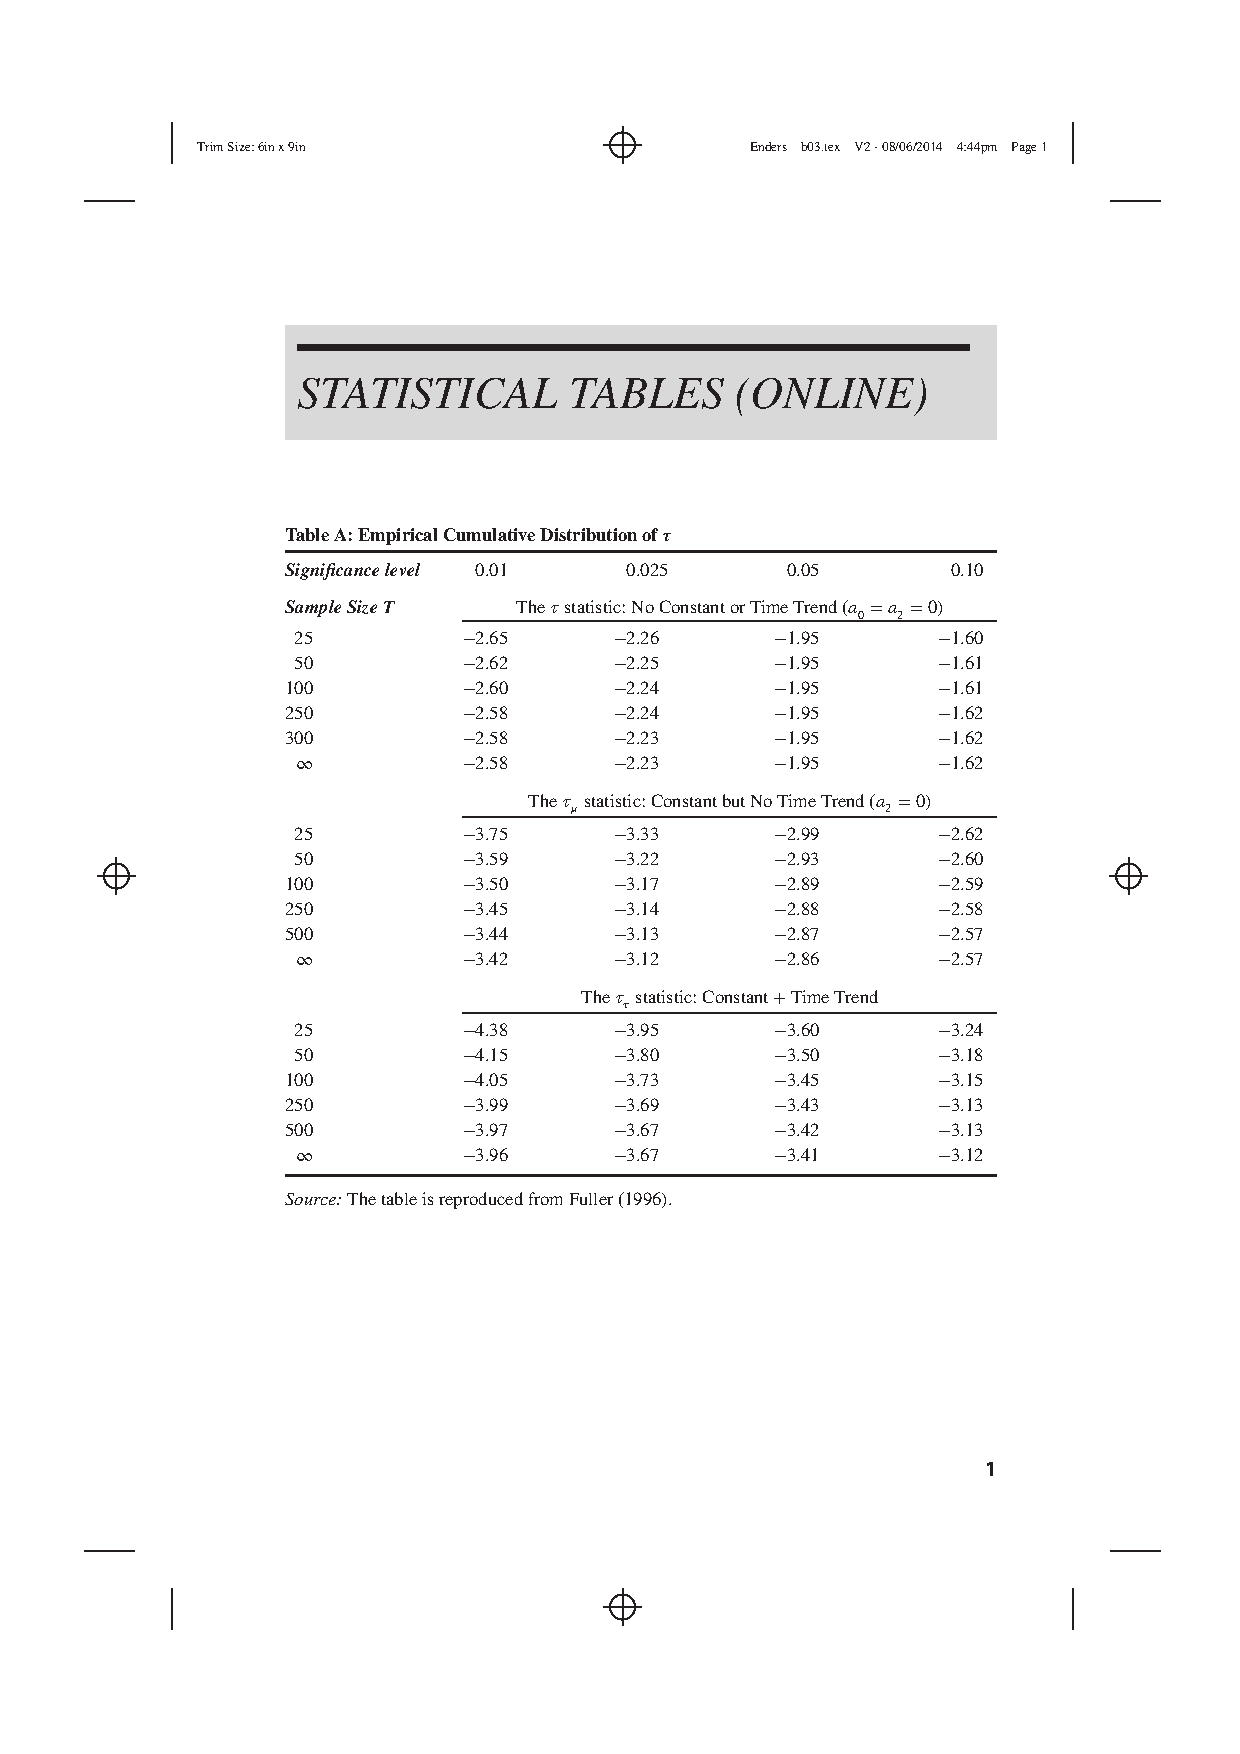
\includepdf[pages=1,pagecommand=\section{Tau-værdier (Kritiske værdier)}]{statistical_table}
\includepdf[pages=2 ]{statistical_table}
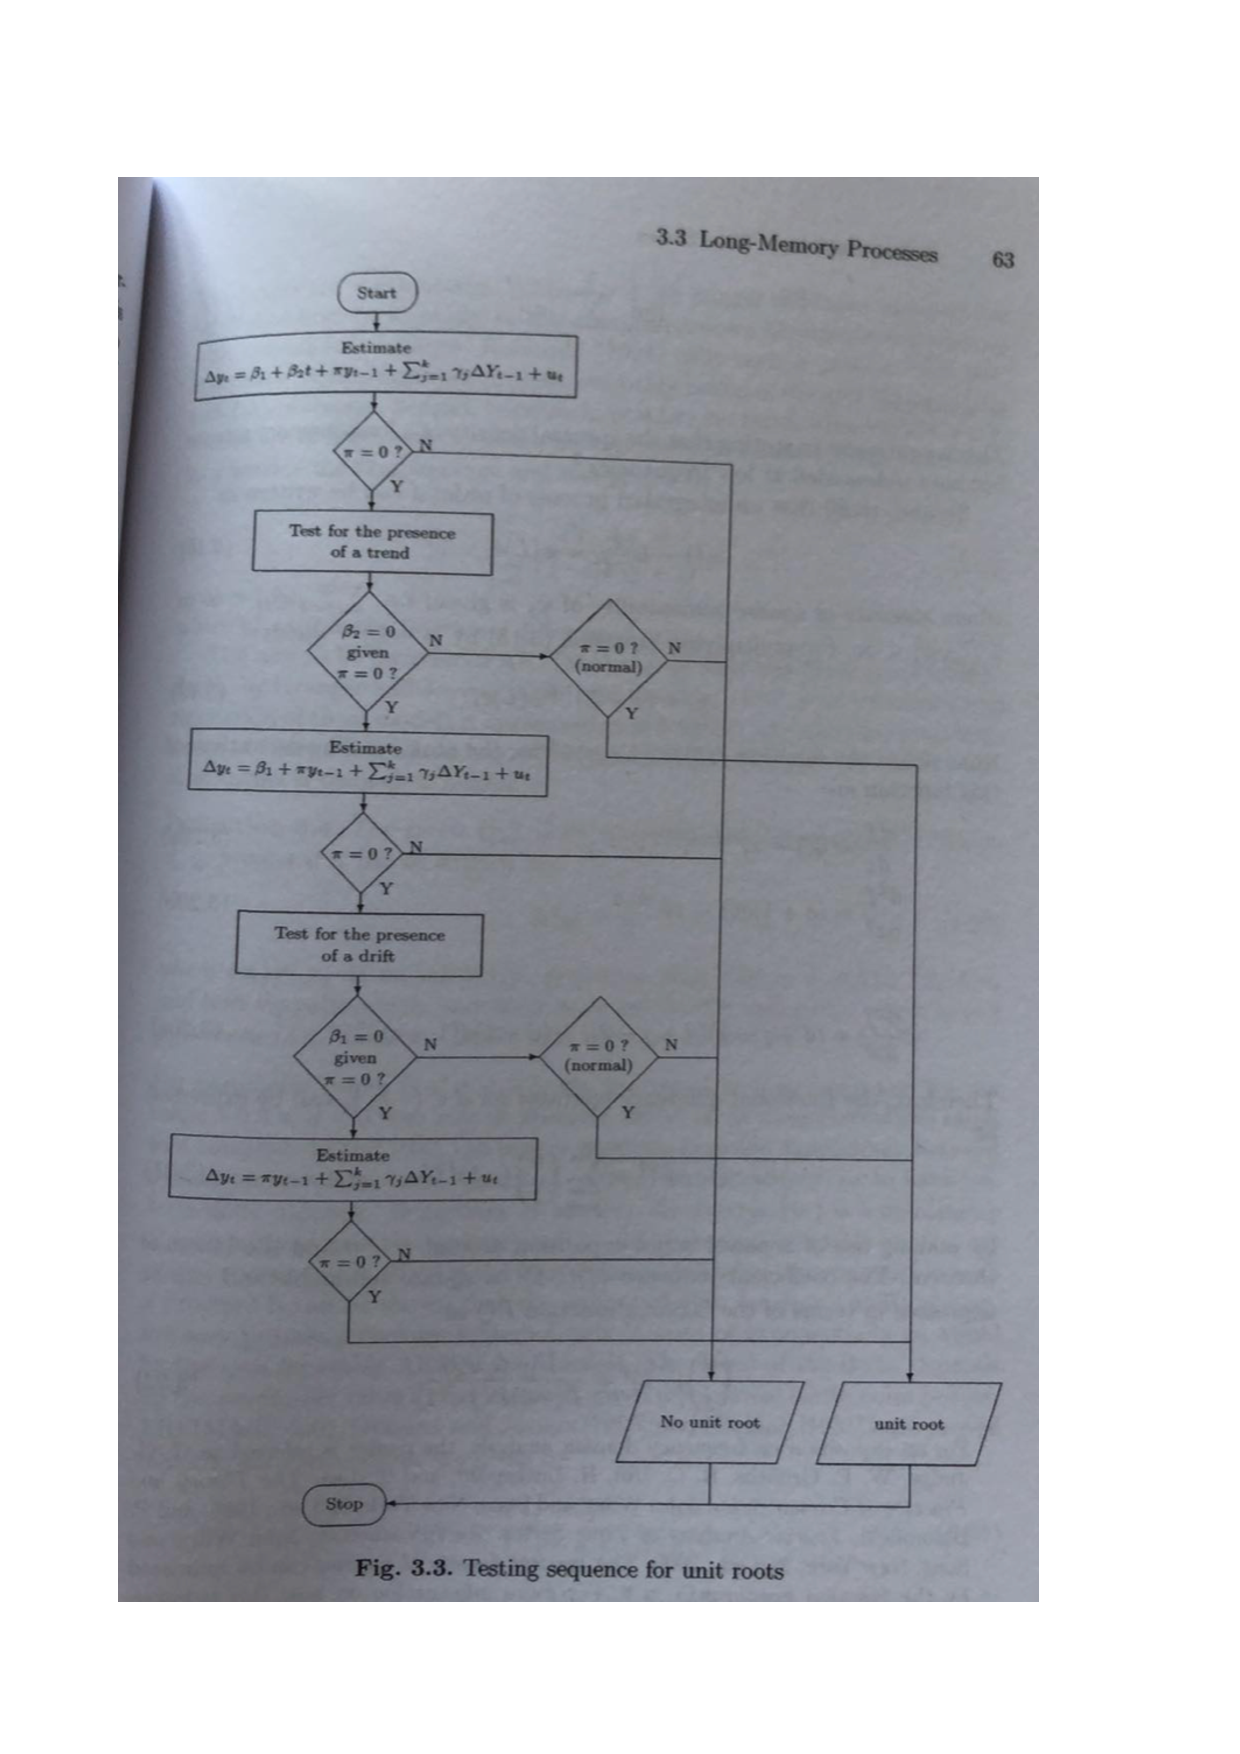
\includepdf[pages=1,pagecommand=\section{Sequential process}]{pfaff_figur_3.3}

\hypertarget{litteraturliste}{%
\section{Litteraturliste}\label{litteraturliste}}

~BIS. (2017). Range of practices in implementing the countercyclical
capital buffer policy. \url{https://www.bis.org/bcbs/publ/d407.htm}.

~Borio, C. (2012). The Financial cycle and macroeconomics: What have we
learnt?. BIS Working Papers nº 395.

~Byrialsen, M. R., Raza, H., \& Stamhus, J. (Accepted/In press).
Exploring the macroeconomic effects of unemployment benefits. Review of
Political Economy.

~Byrialsen, M. R., \& Raza, H. (Accepted/In press). Household debt and
macroeconomic stability: An empirical stock-flow consistent model for
the Danish economy. Metroeconomica.
\url{https://doi.org/10.1111/meca.12358}

~Eriksen, J., \& Etzerodt, S. F. (2019). Time-series cross-section
analyser i komparativ politisk økonomi. Metode \& Forskningsdesign, 3,
24-55. \url{https://journals.aau.dk/index.php/mf/article/view/3400}

~Enders, W. (2015). Applied econometric time series. New York: Wiley.

~Klitgaard, A. G., \& Ehmsen, J. S. (2020). Den finansielle cyklus og de
realøkonomiske effekter.

~Kotzé. (2019). Kevin Kotzé. Kevinkotze. Retrieved January 2, 2022, from
\url{https://www.economodel.com/time-series-analysis-2019}

~Hanson, M. S. (2004). The ``price puzzle'' reconsidered. Journal of
Monetary Economics, 51(7), 1385--1413.
\url{https://doi.org/10.1016/j.jmoneco.2003.12.006}

~Ravn, M. O., \& Uhlig, H. (2002). On adjusting the hodrick-prescott
filter for the frequency of observations. Review of Economics and
Statistics, 84(2), 371--376.
\url{https://doi.org/10.1162/003465302317411604}

~Qanas, J., \& Raza, H. (Accepted/In press). Does securitisation make
monetary policy less effective? Review of Political Economy.

~Sims, C. A. (1980). Macroeconomics and Reality. Econometrica, 48(1),
1--48. \url{https://doi.org/10.2307/1912017}

~Zivot, E. and Andrews, Donald W.K. (1992), Further Evidence on the
Great Crash, the Oil-Price Shock, and the Unit-Root Hypothesis, Journal
of Business \& Economic Statistics, 10(3), 251--270.\\

\end{document}
